\documentclass[a4paper, 9pt, landscape]{article}
\usepackage[scaled=0.92]{helvet}
\usepackage{multicol}
\usepackage{calc}
\usepackage{ifthen}
\usepackage[landscape]{geometry}
%\usepackage{hyperref}

\usepackage{newtxtext} 

%for strikeout
\usepackage{ulem}

%For editing parbox
\usepackage[table]{xcolor}
%For editing itemise margins, reduce iterm separaion and list separation
\usepackage{enumitem}
% For math
\usepackage{amsmath,amsthm,amsfonts,amssymb}

% Verbatim
\usepackage[utf8]{inputenc}
\usepackage{alphabeta}


%For pictures / figures
\usepackage{color,graphicx,overpic}
\graphicspath{ {./images/} }

%\usepackage{newtxtext} 
%\usepackage{amssymb}
%\usepackage[table]{xcolor}
%\usepackage{vwcol}
%\usepackage{tikz}
%\usepackage{wrapfig}
%\usepackage{makecell}

\pdfinfo{
  /Title (CS2109S.pdf)
  /Creator (Ger Teck)
  /Author (Ger Teck)
  /Subject ()
  /Keywords (tex)}

%% Margins for PAPER

% This sets page margins to .5 inch if using letter paper, and to 1cm
% if using A4 paper. (This probably isn't strictly necessary.)
% If using another size paper, use default 1cm margins.
%\ifthenelse{\lengthtest { \paperwidth = 11in}}
%	{ \geometry{top=.2in,left=.2in,right=.2in,bottom=.2in} }
%	{\ifthenelse{ \lengthtest{ \paperwidth = 297mm}}
%		{\geometry{top=1cm,left=1cm,right=1cm,bottom=1cm} }
%		{\geometry{top=1cm,left=1cm,right=1cm,bottom=1cm} }
%	}

%% Margins for A4 PAPER
\geometry{top=0.3cm,left=0.3cm,right=0.3cm,bottom=0.3cm}


% Turn off header and footer
\pagestyle{empty}

% for tight centres (less spacing)
\newenvironment{tightcenter}{%
  \setlength\topsep{0pt}
  \setlength\parskip{0pt}
  \begin{center}
}{%
  \end{center}
}

% Redefine section commands to use less space
\makeatletter
\renewcommand{\section}{\@startsection{section}{1}{0mm}%
                                {-1ex plus -.5ex minus -.2ex}%
                                {0.5ex plus .2ex}%x
                                {\normalfont\large\bfseries}}
\renewcommand{\subsection}{\@startsection{subsection}{2}{0mm}%
                                {-1explus -.5ex minus -.2ex}%
                                {0.5ex plus .2ex}%
                                {\normalfont\normalsize\bfseries}}
\renewcommand{\subsubsection}{\@startsection{subsubsection}{3}{0mm}%
                                {-1ex plus -.5ex minus -.2ex}%
                                {1ex plus .2ex}%
                                {\normalfont\small\bfseries}}
% change font
%\renewcommand{\familydefault}{\sfdefault}
%\renewcommand\rmdefault{\sfdefault}
\makeatother

% Define BibTeX command
\def\BibTeX{{\rm B\kern-.05em{\sc i\kern-.025em b}\kern-.08em
    T\kern-.1667em\lower.7ex\hbox{E}\kern-.125emX}}

% Don't print section numbers
\setcounter{secnumdepth}{0}

\setlength{\parindent}{0pt}
\setlength{\parskip}{0pt plus 0.5ex}

%% this changes all items (enumerate and itemize, reduce margins)
\setlength{\leftmargini}{0.5cm}
\setlength{\leftmarginii}{0.5cm}
\setlist[itemize,1]{leftmargin=2mm,labelindent=1mm,labelsep=1mm, itemsep = 0.5mm, before=\justifying}
\setlist[itemize,2]{leftmargin=3mm,labelindent=0.5mm,labelsep=1mm, itemsep = 0mm, topsep=0mm, before=\justifying}
%\setlist{nosep}

\usepackage[document]{ragged2e}

% -------------------------------------------------------------------------------

% START OF DOCUMENT HERE

\begin{document}
\raggedright
\footnotesize
\begin{multicols*}{3}

% multicol parameters
% These lengths are set only within the two main columns
\setlength{\columnseprule}{0pt}
\setlength{\premulticols}{1pt}
\setlength{\postmulticols}{1pt}
\setlength{\multicolsep}{2pt}
\setlength{\columnsep}{2pt}

\section{CS2109S Introduction to AI. and ML}
\centerline{AY24/25 Sem 2. github.com/gerteck}
• \textbf{Search Algorithms} (Uninformed Search (BFS/DFS), Local Search (Hill Climbing), Informed Search (A*), Adversarial Search (Minimax)) \\
• \textbf{"Classical" ML} (Decision Trees, Linear/Logistic Regression, Kernels and Support Vector Machines, "Classical" Unsupervised Learning) \\ 
• \textbf{"Modern" ML} (Neural Networks, Deep Learning, Sequential Data)


\subsection{1. \underline{Introduction to AI}}

\subsubsection{Intelligent Agent and Environments}
An agent perceives environment through sensors, act through actuators. \\
\textit{Rational}: choose actions to maximize expected performance. 
\begin{itemize}
\item \textbf{Percept}: content agent’s sensors are perceiving. \textbf{Percept Sequence} complete history of things agent has perceived.
\item \textbf{PEAS}: Performance Measure (definition of success), Environment (world agent operates in), Actuators (actions agent can perform), Sensors (Inputs agent gets from environment)\\
(E.g. Chatbot: Sensor as text input/chat history, Actuators as output, Environment as chat interface, plugins, Perf. measure as correctness safety.)
\item \textbf{Exploration vs. Exploitation}: Exploration: learn more about world. Exploitation: Maximize gain based on current knowledge.
\end{itemize}

\subsubsection{Properties of Task Environments}
	\textbf{Observable}: Fully vs. Partially observable.\\
	 \textbf{Deterministic vs. Stochastic}: Next state determined by current state and action. If environment also dependent on actions of other agents, also \textit{strategic}, unless other agents are predictable. \\
	\textbf{Episodic vs. Sequential}: Single-step vs. multi-step tasks. (Next episode does/does not depend on actions taken in previous episode.)\\ 
	\textbf{Static vs. Dynamic}: Environment changes while deliberating. - semi-dynamic (env no change, only change agent performance score) \\
	\textbf{Discrete vs. Continuous}: Finite (distinct, clearly defined) vs. infinite (states/percepts)/actions. \\
	\textbf{Single-agent vs. Multi-agent}: Operating alone or with others.

\subsubsection*{Common Agent Structures}
\textbf{Simple Reflex Agent}: Condition-action rules (e.g., "If up empty: up"). Based on current percept, ignore percept history.\\
\textbf{Goal-Based Agent}: Acts to achieve goals. Tracks state of world, goals.\\
\textbf{Utility-Based Agent}: Maximizes utility (e.g., rewards). Use utility function (perf. measure) to assign scores.\\
\textbf{Learning Agent}: Adapts and improves over time, using performance element, critic and problem generator.

\subsection{2. \underline{Problem Solving by Searching}}
\subsubsection{Search Problem}
Search problem defined where goal is to find state/(path to state) from a set of possible states. \\
\textbf{State Space}. Set of possible states environment can be. \\
\textbf{Representation Invariant}: Abstract states hv. mapped concrete states.
\textbf{Initial State} where agent starts, \textbf{Goal State(s)}: can be $>$ 1, use goal test. \\
\textbf{Actions}. Given state $s$, finite set of actions that can be executed. \\
\textbf{Transition Model}. Describes what each action does. Returns state resulting from action $a$ in state $s$. \\
\textbf{Action Cost Function}: Numeric cost of applying action to reach next state. \\
\textbf{Search Algorithm}: Takes search problem as input, returns a solution / failure. Solution could be sequence of actions, or final state. Optimal solution is one with least cost.

\subsubsection{Search Algorithms}
Search algorithms explore the state space to find solution. Key operations: \\
\textit{Frontier}: Set of nodes to explore next. \textit{Explored Set}: Nodes already visited. \textit{Node}: Contains state, parent node, action, path cost, and depth.
 \\ \smallskip
 \textbf{Performance/Evaluation} \\
 \textit{Completeness}: Finds solution if exists / report failure for none. \\
\textit{Optimality (Cost) }: If outputs solution, it is lowest path cost of all solutions. Algorithm can be both optimal and incomplete. \\
\textit{Time, Space complexity}: How long, how much memory needed. 

\subsubsection{Uninformed Search Algorithms}
No information to guide search, aka blind search, no clue how good state is. \\
\smallskip
\textbf{Breadth-First Search (BFS)}
\begin{itemize}
    \item \textbf{Frontier}: Queue (FIFO). Explore all nodes at curr. depth, before deeper.
    \item \textbf{Complete}: if branching factor $b$ finite. \textbf{Optimal}: if step cost uniform.
    \item \textbf{Complexity}: Time: $O(b^d)$, $d$ is depth of shallowest sln. Space: $O(b^d)$.
    \item \textit{Optimize}: track visited set, early goal test (check node soln once generated).
\end{itemize}
\smallskip
\textbf{Uniform-Cost Search (UCS) (Dijkstra's SSSP 'equiv')}
\begin{itemize}
    \item \textbf{Frontier}: Priority queue by min total path cost. Expand least-cost first.
    \item No-visited-mem ('tree-search', as if tree). Visited-mem ('graph-search').
    \item Even if goal state in frontier, sorted, first g-state selected must be optimal.
    \item \textbf{Complete}: if step costs are positive. \textbf{Optimal}: if step costs are positive.
    \item \textbf{Complexity}: Time: $O(b^{C^*/\epsilon})$, $C^*$ is the optimal cost, $\epsilon$ is minimum step cost. Space: $O(b^{C^*/\epsilon})$. (w.r.t `tier' of optimal solution)
\end{itemize}
\smallskip
\textbf{Depth-First Search (DFS)}
\begin{itemize}
    \item \textbf{Frontier}: Stack (LIFO). Explores as deep as possible before backtrack.
    \item \textbf{Incomplete}: if search tree has infinite depth or loops. \\\
     \textbf{Non-optimal}: No, may find suboptimal solutions.
    \item \textbf{Complexity}: Time: $O(b^m)$, where $m$ is max depth. Space: $O(bm)$.
\end{itemize}
\smallskip
\textbf{Depth-Limited Search (DLS)}
\begin{itemize}
    \item Limit search depth to $l$. Backtrack when limit hit. Good if opt. $d$ known.
    \item \textbf{Incomplete}: if sln exists beyond depth $l$. \textbf{Non-optimal}: if used w. DFS.
    \item \textbf{Complexity}: Time: $O(b^l)$. Space: $O(bl)$.
\end{itemize}
\smallskip
\textbf{Iterative Deepening Search (IDS)}
\begin{itemize}
    \item Repeatedly applies DLS with increasing depth limits. Try all possible depth limits from 0 till sln found or failure value returned from DLS. Combines benefits of BFS and DFS.
    \item \textbf{Complete}: If branching factor $b$ finite. \textbf{Optimal}: if step costs uniform.
    \item \textbf{Complexity}: Time : $O(b^d)$. Space: $O(bd)$.
\end{itemize}

\subsubsection{Informed Search Algorithms}
Guide search with extra info, aka heuristic function on how close to goal. \\
\textbf{Heuristic} $h(n)$ estimates cost to reach goal from node $n$. $h^*(n)$: true cost.
\begin{itemize}
\item \textbf{Admissible}: Never overestimates cost ($h(n) \leq h^*(n)$). (e.g. $h(n)=0$) 
\item \textbf{Consistent}: if for every node $n$, every successor $n'$ of $n$ generated by any action $a$:
   $h(n) \leq c(n, a, n') + h(n')$ and $h(G) = 0$. $\Delta$ Inequality.
\item \textit{Relaxed Problem}: Problem w. fewer restrictions. Cost of optimal solution to relaxed problem is admissible heuristic for original problem. (e.g. straight line distance for cities distances).
\item \textit{Dominance}: If $h_1(n) \geq h_2(n)$ for all $n$, $h_1$ dominates $h_2$. Dominant heuristics better for search if admissible. (e.g. straight line distance, vs trivial heuristic $h = 0$.)
\end{itemize}
\columnbreak

\textbf{Best-First Search}
\begin{itemize}
    \item \textbf{Frontier}: Priority queue ordered by evaluation function $f(n)$. Expands most promising node based on just $f(n)$ (no past cost).
    \item Not complete, not cost-optimal.
\end{itemize}

\smallskip
\textbf{A* Search}
\begin{itemize}
    \item \textbf{Frontier}: Priority queue. (Best-First Search considering path cost).
    \item Use evaluation $f(n) = g(n) + h(n)$. $g(n)$ is cost to reach $n$ from start. $h(n)$ is estimated cost to reach goal from $n$.
    \item \textbf{Complete}: if $h(n)$ is admissible, state space finite, step costs positive. \textbf{Optimal} if $h(n)$ is admissible.
    \item \textbf{Complexity}: Time: Exponential but improved by good heuristics. Space: Exponential. (Both $O(b^d)$ for poor heuristic.)
\end{itemize}
If $h(n)$ admissible, A* search (w/o visited memory) is optimal. If $h(n)$ consistent, A* search (w. visited memory) is optimal.
\\ \smallskip
• A consistent heurisitic $\implies$ admissible (T2.QnC.1). Converse not true.\\
• (Trivial $h=0$ consistent, admissible) \\
• Triangle inequality: Sum of lengths of any two sides $\geq$ length of $3^{rd}$ side.


\subsection{3. \underline{Local Search}}
For (NP-hard) problems,  traverse state space in systematic manner not option, is intractable (unsolvable in time). \\ \smallskip
\textbf{Local Search}: Explore state space considering only locally-reachable states ('search space').  Start random position, iterative move to neighboring states via perturbation or construction. Solution is final state, not path taken. \\
(E.g. N-Queens Problem, minimize function value) 
\begin{itemize}
\item Typically incomplete and suboptimal. 
\item \textit{Any-time property}: Longer runtime yields better solutions. Suitable for obtaining "good enough" solutions for difficult problems.
\item \textbf{Types}: \textit{Perturbative} Search (search space is complete solutions, modify components of current solution). \textit{Constructive} Search (partial candidate solutions, extend by adding components).
\end{itemize}
\textbf{Problem Formulation in Local Search}: \\
\textit{States}: Represent configurations/candidate sln within search space, but may not directly map to actual state. \textit{Goal Test} (Optional) checks if current state is desired solution. \textit{Successor Function}: Generates neighboring states by applying small modifications. \\
\textbf{Evaluation/Objective Function}: assess quality of state, max/minimize based on problem. (E.g. N-Queen Maximize "safe" queens, min. y value.)

\subsubsection{Hill-Climbing Algorithm}
Find local maxima by travelling to neighbouring states with highest value, terminate when no neighbour has higher value. 
One objective function is to negate heuristic function.
\begin{verbatim}
current_state = initial_state
while True:
    best_successor = highest-valued successor of curr_state
    if eval(best_successor) <= eval(current_state):
        return current_state
    current_state = best_successor
\end{verbatim}
\textbf{Greedy local search}: gets stuck at local maxima, ridges, plateaus, shoulders (same values flat area). Some solutions include limited sideways move, stochastic (probability based on steepnes of move), first-choice, random-restart. Simulated Annealing - allow occasional 'bad moves' to escape local optima.


%% CAN ADD SOME STUFF HERE %%

\columnbreak

\subsection{4. \underline{Adversarial Search and Games}}
\textbf{`Classicial' Adversarial}: Agents/Player compete against each other. Look at deterministic, two player, turn-taking, perfect information, zero-sum games. Perfect information: fully observable. Zero sum: no “win-win”. 
\begin{itemize}[itemsep=-2pt]
\item \textit{States}: Configurations of game, initial state, terminal state (win/lose/draw). 
\item \textit{Actions}: Possible moves by a player.
\item \textit{Transition Model}: Defines how actions change the state. 
\item \textit{Utility Function}: Assigns a value to terminal states from perspective of the agent. (E.g. Win: $ +1 $, Draw: $ 0 $, Loss: $ -1 $)
\end{itemize}


\subsubsection{Minimax Algorithm}
Determine optimal move for Player A (MAX) assuming Player B (MIN) plays optimally. Work out minimax value of each state in tree.
\begin{itemize}
	\item \textbf{Complexity}: Time: Exponential w.r.t. max depth ($ O(b^m) $). Space: Poly.
	\item \textbf{Complete}: If tree is finite. \textbf{Optimal} if against optimal opponent.
\end{itemize}
It is a recursive algo, backs up minimax values as recursion unwinds. Thus, similar to DFS, time c. $ O(b^m) $, space c. $O(bm)$. \\
\textit{Note}: minimax not 'optimal' against non-optimal MIN player, as non optimal player could choose higher value in unchosen path (which had lower min value). But guarantees it never lower utility than of optimal opponent.

\subsubsection{Alpha-Beta Pruning (Minimax)}
Reduces number of nodes (computational overhead) evaluated in game tree without affecting final decision. Minimax no need explore full tree. Good move ordering improves effectivness of pruning.
\begin{itemize}[itemsep=-2pt]
        \item $ \alpha $: MAX's highest guaranteed so far. MAX updates α. 
        \item $ \beta $: MIN's lowest guarantee so far. MIN updates β. 
	\item At MAX node, prune (stop) if α $\geq$ β. At MIN node, prune (stop) if β $\leq$ α. 
	\item Values of α, β passed down tree as explore nodes. \\
	When backtracking, values passed up to update α, β if applicable.
\end{itemize}
Good move ordering improves effectivness of pruning.

\subsubsection{Evaluation Function to Cutoff (Minimax)}
Fully exploring game tree with Minimax may be computationally infeasible.
\begin{itemize}[itemsep=-2pt]
    \item Apply \textbf{cutoff strategy} to halt the search at predefined maximum depth. 
    \item Use \textbf{heuristic function} to estimate the utility of mid-game (non-terminal) states. Heuristic must be some value between win and loss, and computationally efficient. Admissibility, consistency properties do not apply. Can use domain-specific features or some labeled dataset to train heuristics.
\end{itemize}


\subsection{5. \underline{Machine Learning}}
Computers with ability to learn without explicit programming, through algorithms that learn from, and make predictions based on data. Goal is for performance to improve over time by identifying patterns in the data.
\subsubsection{Problem Types}
\begin{itemize}[itemsep=-2pt]
\item \textbf{Classification}: Output category value in finite set. (Predict discrete label)
\item \textbf{Regression}: Output is number. (Predict continuous num. value)
\end{itemize}

\subsubsection{Types of Machine Learning (Feedback difference)}
\begin{enumerate}[itemsep=-2pt]
    \item \textbf{Supervised Learning}: Learns from labeled data (input-output pairs) to map inputs to outputs. (E.g. classify pic banana or apple)
    \item \textbf{Unsupervised Learning}: Learns from unlabeled data to find patterns or structure. (E.g. clustering, group based on features).
    \item \textbf{Semi-Supervised Learning}: Use labeled, unlabeled data for learning.
    \item \textbf{Reinforcement Learning}: Learns to make decisions by interacting with an environment, (rewards and penalties).
\end{enumerate}

\subsection{\underline{Supervised Learning {\scriptsize (Decision Trees, Linear/Logistic Regression, SVMs)}}}
\begin{itemize}[itemsep=-2pt]
    \item \textbf{Training Phase}: Map inputs to output, using train data. Result: \textit{model / hypothesis}.
    \item \textbf{Testing Phase}: Model's performance on test data to evaluate generalization.
    \item Supervised learning: dataset represented as set of pairs $(x^{(i)}, y^{(i)})$:
    {
	\setlength{\topsep}{0pt}
	\setlength{\partopsep}{0pt}
    \begin{itemize}[itemsep=-2pt]
	    \item $ x^{(i)} \in \mathbb{R}^d $: Input vector of $ i $-th data point with $ d $ features.
	    \item $ y^{(i)} $: Label (target) for the $ i $-th data point. $( y^{(i)} \in \mathbb{R} \text{ or} \in \{1, \dots, C\}) $
	    \item Dataset $ D $ with $ n $ examples: $ D = \{(x^{(1)}, y^{(1)}) \dots, (x^{(n)}, y^{(n)})\} $.
	\end{itemize}
	}
\end{itemize}
\textbf{Goal}: to find hypothesis $h(x)$ that approximates the true function $f^*$, assuming an unknown true relationship $y = f^*(x) + \epsilon$, $\epsilon$ noise error term.
\begin{itemize}[itemsep=-2pt]
	\item \textbf{Hypothesis class $ \mathcal{H} $}: set of all possible learnable models or functions. \\
	 Each $ h \in \mathcal{H} $ is a hypothesis or model. (Classes - e.g DT, linear model, NN).
	 \item \textbf{Performance Measure}: Test hypothesis on new set (test set). Metrics:
        \begin{itemize}[itemsep=-1.5pt]
            \item (Regression) Mean Squared Error (MSE), Mean Absolute Error (MAE).
            \item (Classification) Accuracy: $ \text{Accuracy} = \frac{1}{N} \sum_{i=1}^N \mathbf{1}(\hat{y}^{(i)} = y^{(i)}) $.
            \item (Classification) Confusion Matrix: Precision ($\frac{TP}{TP + FP}$ - opt if FP costly), \\
            Recall ($\frac{TP}{TP + FN}$ - opt if FN costly), F1 Score: $\frac{2}{\frac{1}{P} +\frac{1}{R}} $
        \end{itemize}
        \item \textbf{Generalization}: Model performance on unseen data. Depends on train dataset quality/quantity (relevance, noise, balance), model complexity.
        \begin{itemize}
			\item \textbf{Bias}: Error stems from model too simple. Model w. high bias fails to capture patterns in data, leading to underfitting. Error does not reduce with more data.
			\item \textbf{Variance}: Error stems from model too sensitive to small fluctuations in training data. Captures noise, lead to overfitting. Error reduces more data.
			\item Simple models tend to have high bias, low variance while complex models have low bias, but high variance. Otherwise, data with significant outliers , weak classifiers, etc can affect bias, variance as well.
		\end{itemize}
        \item \textbf{Hyperparameter Tuning}: Adjust params (e.g. $\gamma$) to optimize performance. Predefined before training. Hyperparam search: grid (exhaustive), random etc. 
\end{itemize}


\subsection{6. \underline{Decision Trees}}
Function input: vector of attribute values. Outputs single value (decision). Perform sequence of tests from root node to leaf.
\begin{itemize}
\item \textbf{Expressiveness}: Can express any (propositional) fn of input attributes. 
\item \textbf{Size of Hypothesis Class}: Distinct decision trees, $ n $ bool. attributes: $2^{2^n}$
\item \textbf{Decision Tree Learning}: Greedy, top-down, recursive algorithm. Use information gain, choose best attribute to divide training set. For each value of chosen attr. use DTL again on corresponding subset of examples.
\item \textbf{Entropy}: $I(P(v_1), P(v_2), ..., P(v_k)) = - \sum_{i=1}^{k} P(v_i) \log_2 P(v_i)$
\item \textbf{Information Gain}: Initial Entropy $-$ avg. entropy after divide `remainder'. \\
Entropy before dividing: $I(\frac{p}{p+n},\frac{n}{p+n})$, $p + n$ examples in subset $E_i$.
\end{itemize}


\subsubsection{Information Gain}
Given \textit{attribute} $A$ with $v $ distinct values, the training set is split into subsets $ E_1, ..., E_v $, each with \( p_i \) positive and \( n_i \) negative examples. Choose attribute with max information gain.
\begin{itemize}
\item $\text{remainder}(A) = \sum_{i=1}^{v} \frac{p_i + n_i}{p+n} I\left(\frac{p_i}{p_i+n_i}, \frac{n_i}{p_i+n_i} \right)$
\item $\text{Info Gain: } IG(A) = I(p_{\text{pos}}, p_{\text{neg}}) - \text{remainder}(A)$
\end{itemize}
\textbf{Decision Tree Overfitting / Generalization}: 
\begin{itemize}
\item \textbf{Prune Decision Tree}: Smaller tree may have higher accuracy due to noise ignored.
	\begin{itemize}
	\item \textbf{min-sample leaf} (min threshold of sample count in leaf node) 
	\item  \textbf{max depth} (longest path from root to leaf) pruning. 
	\end{itemize}
\item \textbf{Data Preprocessing}: Missing values (assign most common value, drop row/attribute etc.) Continuous values - partition to discrete set as attribute.
\end{itemize}
 

\subsection{7. \underline{Linear Regression  $\rightarrow$ Regression (Prediction) Tasks}}

\textbf{Linear Model}: Input vector $x$ of dimension $d$, hypo class is set of linear fns:
\[h_w(x) = w_0x_0 + w_1x_1 + w_2x_2 + \dots + w_dx_d\  = w^T x. \] 
where $ w_0 \text{($\leftarrow$ bias term)}, w_1, \dots, w_d $ are weights, $ x_0 = 1 $, dummy variable.

\centerline{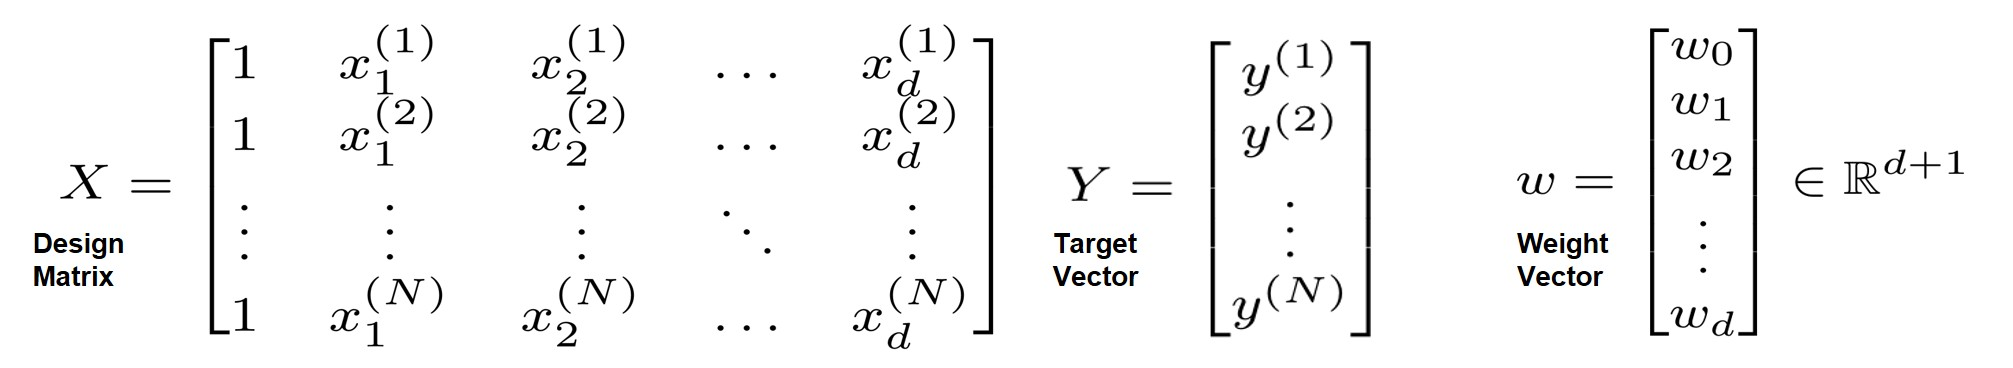
\includegraphics[width=1\linewidth]{matrix}}
• $X \in \mathbb{R}^{N \times (d+1)} | w \in \mathbb{R}^{d+1} | Y, \hat{Y} \in \mathbb{R}^N $ (target, predicted values).
\begin{itemize}
\item \textbf{Feature Transformations}: modify features for better modeling. Feature Engineering (e.g. poly $ z = x^k $/ log $ z = \log(x) $/ exp). Feature scaling (e.g. min-max scaling $ z_i = \frac{x_i - \min(x_i)}{\max(x_i) - \min(x_i)} $, standardization $ z_i = \frac{x_i - \mu_i}{\sigma_i} $). 
\item \textbf{Measure Fit}: Loss fn of weights $w$, find $w$ to min. loss. ($N: \#$ train pts)
\item \textbf{Loss Fn}: $J_{MSE}(w) = \frac{1}{2N} \sum_{i=1}^N (h_w(x^{(i)}) - y^{(i)})^2.$
\item \textbf{Derivative}:$\frac{\partial J_{MSE}(w)}{\partial w_j} = \frac{1}{N} \sum_{i=1}^N \big(h_w(x^{(i)}) - y^{(i)}\big) x_j^{(i)}$
\end{itemize}

\textbf{Learning via Normal Equation}: Solve for $ w $ that minimizes $ J_{MSE} $:    $w = (X^T X)^{-1} X^T Y$. However, problem that computational cost: $ O(d^3) $ for matrix inversion. Non-linear models cannot be solved using normal equations. \\ \smallskip


\textbf{Learning via Gradient Descent}: 
\begin{itemize}[itemsep=-2pt]
    \item \textbf{Algorithm}: Initialize $ w $ randomly. Update weights iteratively. \\
     Repeat until convergence: $w_j \leftarrow w_j - \gamma \frac{\partial J(w_0, w_1, \dots)}{\partial w_j}.$
    \item \textbf{Learning rate} $ \gamma > 0 $: Controls step size. (Hyperparameter). can $\downarrow$ w time.
    \item \textbf{Variants}: Batch, use all data points. Mini-batch, use data subsets. Stochastic, uses one data point per iteration.
    \item \textbf{Convex}: MSE loss fn. convex, single global min, for linear/poly regression. 
\end{itemize}

\subsection{8. \underline{Logistic Regression  $\rightarrow$ Classification Tasks}}
\textbf{Logistic Regression Model}: Hypo class: Set of "squashed" linear fns. 
\begin{itemize}[itemsep=-2pt]
    \item \textbf{Sigmoid function}: $\sigma(x) = \frac{1}{1 + e^{-x}}$, \quad $\frac{\partial \sigma}{\partial x}: \sigma'(x) = \sigma(x)(1 - \sigma(x))$
    \item Logistic model: $h_w(x) = \sigma(w_0x_0 + w_1x_1 + \dots + w_dx_d) = \sigma(w^T x)$ \\
    where $ w_0, w_1, \dots, w_d $ are weights, $ x_0 = 1 $ is a dummy variable.
\end{itemize}
\textbf{Classification with Logistic Regression}: Regression outputs value in $ [0, 1] $, treat as probability of class 1. (E.g. $ h_w(x) = 0.8 $ predicts 80\% chance of failure). Use \textbf{Decision threshold} (e.g. 0.5) for classification.  \\
\textbf{Desn. Boundary}: surface (e.g. 2D line) separating classes in feature space.\\
\textbf{Non-Linearly Separable Data}: If single linear decision boundary cannot separate classes, use non-linear models or apply non-linear feature transformations. \\
\textbf{Evaluation Metric}: Use Accuracy. Don't use BCE, MSE, MAE, (loss functions).

\subsubsection{Logistic Regression Loss Function}
Use \textbf{Binary Cross Entropy} for Loss. MSE not ok for logistic due to non-convexity.
\begin{itemize}[itemsep=-2pt]
    \item $BCE(y, \hat{y}) = -y \log(\hat{y}) - (1 - y) \log(1 - \hat{y})$ .
    \item \textbf{BCE} loss is convex for logistic regression. Small loss if $ y \approx \hat{y} $, large loss if $ y $ and $ \hat{y} $ differ - good loss function. 
    \item \textbf{Derivative}: $\frac{\partial J_{BCE}(w)}{\partial w_j} = \frac{1}{N} \sum_{i=1}^N (h_w(x^{(i)}) - y^{(i)}) x_j^{(i)}. $ (same-linear)
    \item \textbf{Weight update} rule: $w_j \leftarrow w_j - \gamma \frac{\partial J_{BCE}(w)}{\partial w_j} $
\end{itemize}

\subsubsection{Multi-Class Classification {\scriptsize (extending Binary classification)}}
Extend binary classification to multiple class by breaking down into sets.
 \textbf{One-vs-one}: Binary classifier for every pair of classes $total =\frac{C(C-1)}{2}$ classifiers. Class with most votes wins. \\
 \textbf{One-vs-rest}: Binary classifier for each class, treat all other classes as combined class. \textbf{$C$ classifiers.} Class with highest probability output wins.

\columnbreak

\subsection{\underline{Regularization} {\scriptsize (Technique to \textbf{reduce overfitting}, \textbf{penalize large weights in model}.) }}
\begin{itemize}[itemsep=-1pt]
\item \textbf{Overfitting} happens when model too complex, captures training data noise over underlying pattern leading to poor generalization on unseen data.
	\begin{itemize}[itemsep=-2pt]
	    \item Often associated w. models w. large weights. E.g. Complex polynomial model may fit train data perfectly but fail to generalize to new data. 
	    Large oscillations in model may occur as weights $ w $ increase, even while fitting same set of points.
	\end{itemize}
\end{itemize}
\textbf{Regularization}: Add penalty term to loss function, discourage large weights.

\begin{itemize}[itemsep=-1pt, topsep=0.5pt]
\item Perform feature scaling before regularization. (Same effect on all variables).
\item Given a loss function $ J(w) $, add penalty function $ P(w) $, hyperparam: $ \lambda \geq 0 $. 
\[\min_w J_{\text{reg}}(w) = J(w) + \lambda P(w)\]
\end{itemize}
\textbf{Penalty Functions}
\begin{itemize}[itemsep=-1pt]
    \item \textbf{L2 (Square, Ridge) penalty/regularizer}: Penalize square of weights. \\
     \textit{Heavily penalize larger parameters}, but \textit{diminishing return} for reducing already small parameters. Shrink params, but not to 0.
    \item \textbf{L1 (Absolute, Lasso) Regularizer}: Penalize absolute weights. Since penalty grows at same rate, if parameter loss reduction not much, optimal sets weight to 0. Effectively does feature selection strategy, by driving some weights to 0.
    {\scriptsize
    \[P_{\text{square}}(w) = \frac{1}{2} \sum_{j=0}^d w_j^2, \quad P_{\text{abs}}(w) = \sum_{j=0}^d |w_j|, \]
	}
    \item \textbf{Others}: E.g. max-norm penalty, constraint max weight to prevent extreme values.
\end{itemize}

\textbf{Regularization: Effect on Learning Algorithms}
\begin{itemize}[itemsep=-2pt]
    \item \textbf{Gradient Descent}: Gradient of regularized loss function has both gradient of original loss, and gradient of penalty term: $\frac{\partial J_{\text{reg}}(w)}{\partial w_j} = \frac{\partial J(w)}{\partial w_j} + \lambda \frac{\partial P(w)}{\partial w_j}.$

    \item \textbf{Normal Equation}: For linear regression with L2 regularization, the closed-form solution becomes:
    $w = (X^T X + \lambda I)^{-1} X^T Y $, where $ I $ is a identity matrix. This ensures invertibility of $ X^T X + \lambda I $, even for multicollinearity or insufficient data.
\end{itemize}

\textbf{Regularization Strength $ \lambda $ Tradeoffs}: Hyperparameter (penalty strength) $ \lambda $ controls trade-off between fitting training data and keeping weights small:
\begin{itemize}[itemsep=-2pt]
    \item Small $ \lambda $: Emphasizes fitting the data, potentially leading to overfitting.
    \item Large $ \lambda $: Emphasizes smaller weights, potentially leading to underfitting.
\end{itemize}

\subsection{\underline{Kernels}: Kernel Method}
In linear models, weights are linear combinations of inputs (consider how weights calculated through normal equation $X^T Y$), relying only on dot products. \\ The \textbf{kernel method} replaces these \underline{dot products} with a \underline{kernel function} $K(x,x')$, enabling powerful nonlinear models without explicit feature mapping.
\begin{itemize}
	\item \textbf{Dot Product and Similarity}: Dot product $[ u \cdot v = u^T v ]$ measures similarity between 2 vectors. E.g. orthogonal vectors dot product of zero: {\tiny$\begin{bmatrix} 1 \\ 1 \end{bmatrix} \cdot \begin{bmatrix} 1 \\ -1 \end{bmatrix} = 0 $}
	\item \textbf{Dual Formulation of Linear Regression:} Linear model $ h_w(x) = w^T x $, dual form is where $ \alpha_j $ are new parameters (weights), and $ x^{(j)} $ are training data points. (Predictions as weighted sum of dot products of training data $ x^{(j)} $ and input $ x $).
	\item \textbf{Dual Formulation with Kernel (Kernel Trick):} We simply replace the dot product $ (x^{(j)})^T x $ with the kernel function $\mathbf{k(x^{(j)}, x)}$.
	\[h_\alpha(x) = \sum_{j=1}^N \alpha_j (x^{(j)})^T x \quad \implies \quad h_\alpha(x) = \sum_{j=1}^N \alpha_j k(x^{(j)}, x)\]
\end{itemize}

\subsubsection{Kernel Trick}
\vspace{-0.5em}
\centerline{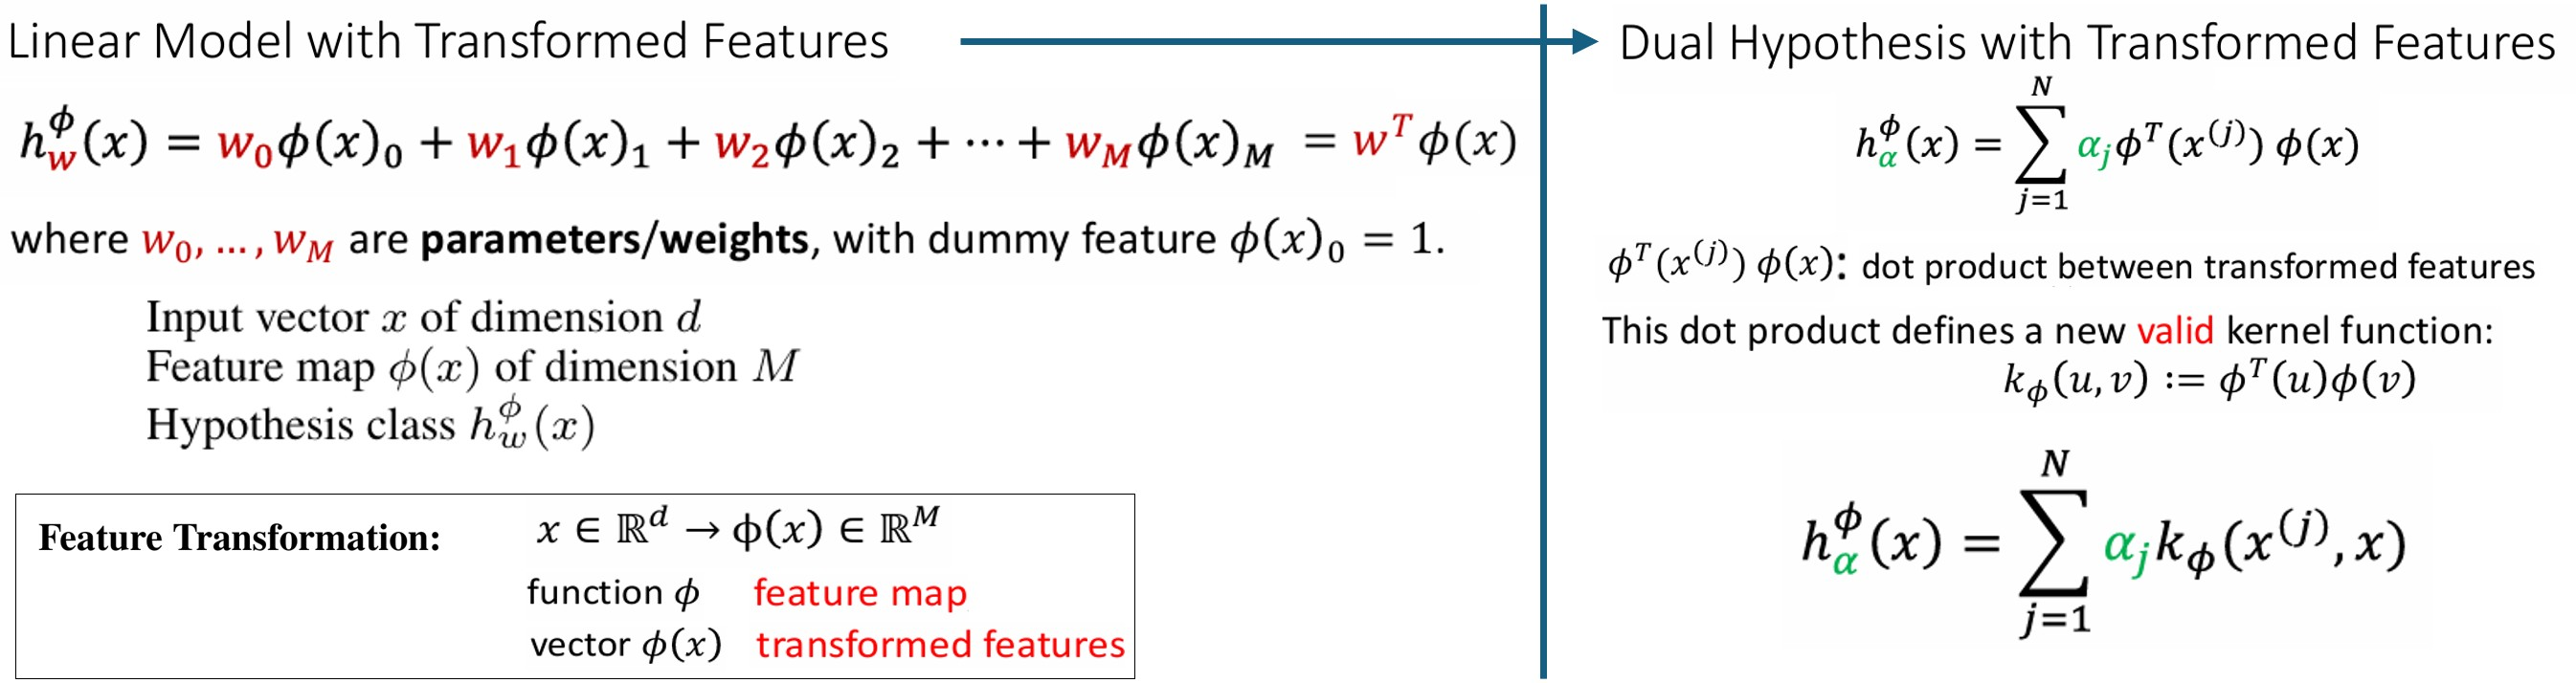
\includegraphics[width=1\linewidth]{kernel}}
\textbf{Kernel function} $ k(u, v) $ generalizes dot product, measures similarity efficiently in potentially higher-dimension space, w/o explicit computing transformation.
\begin{itemize}[itemsep=-1.5pt]
	\item \textbf{Valid kernel functions}: satisfies conditions like symmetry, positive definiteness. 
	\item \textbf{Kernel Machine}:	A model that uses the kernel trick.
	\item The kernel trick allows handling of non-linear data efficiently, enabling efficient computation of complex relationships in data. 
\end{itemize}

\subsubsection{Kernels and Transformed Features}
There is a deep connection between kernels and feature transformations (be it single variable, multi-variable transformations to create new features). Specifically:
\begin{itemize}[itemsep=-2pt]
    \item Any valid kernel $ k(u, v) $ corresponds to a feature map (transform) $ \phi $ s.t.:
    \[
    k(u, v) = \phi(u)^T \phi(v).
    \]
    \item Conversely, any feature transformation $ \phi $ induces a valid kernel.
\end{itemize}


\subsubsection{Examples of Kernels}
\begin{itemize}[itemsep=-1pt]
    \item \textbf{Polynomial Kernel}: {\scriptsize $k(u, v) = (u^T v)^s$ } where $ s $ is degree of polynomial.
    \item \textbf{Gaussian (RBF) Kernel}: 
    \[ k(u, v) = \exp\left(-\frac{\|u - v\|^2}{2 \sigma^2}\right) \]
    \begin{itemize}
		\item where $ \sigma^2 $ controls width of Gaussian ($\downarrow \sigma = $ narrower, $\uparrow \sigma $ = wider).
		\item The RBF kernel corresponds to an infinite-dimensional feature map. Computing $ \phi(x) $ explicitly may be infeasible, but evaluating $ k(u, v) $ efficient.
	\end{itemize}
    \item \textbf{String Kernel}: Measures similarity between strings.
    \item \textbf{Chi-Squared Kernel}: Useful for histograms.
    \item \textbf{Tanh Kernel}: Similar to neural network activation functions.
\end{itemize}

\subsection{9. \underline{Support Vector Machines} (SVM)}
SVM is a powerful classifier that can use kernel tricks (allowing it to handle non-linear decision boundaries naturally) - a kernel machine. 
\begin{itemize}[itemsep=-2pt]
	\item \textbf{Decision boundary}: defined by hyperplane separating points of diff. classes.
	\item \textbf{Margin}: distance between hyperplane and closest data points from each class. The width of the margin is proportional to 2 × margin.
	\item \textbf{Maximizes Margins}: The SVM model is optimized by maximizing the margin subject to constraints that data points are on the correct side of the decision boundary.
	\item \textbf{Support Vectors}: Data points that lie exactly on boundary of margin. These points define position and orientation of hyperplane.
\end{itemize}

\subsubsection{\underline{SVM}: Data, Model and Sparsity}
\begin{itemize}[itemsep=-2pt]
    \item Given $ N $ data points, described by features $ x^{(i)} $, target $ y^{(i)} \in \{-1, 1\} $.
    \item The SVM classifier in dual formulation depends on parameters $ \alpha_i $:
    \[
    \text{SVM}_{\alpha}(x) = \text{sign} \left( \sum_{i=1}^N \alpha_i k(x^{(i)}, x) \right),
    \]
    where $ k(x^{(i)}, x) $ is the kernel function.
    \item \textbf{Sparsity}: Many $ \alpha_1, \alpha_2, \dots, \alpha_N $ will be zero. Only support vectors contribute to classifier. Non-support vectors discarded without affecting model.
    \[    \text{SVM}_{\alpha}(x) = \text{sign} \left( \sum_{i \in \text{Support Vectors}} \alpha_i k(x^{(i)}, x) \right).    \]
    \item \textbf{Implementation}: libraries e.g. \texttt{scikit-learn} to simplify implementation.
\end{itemize}

\subsubsection{Hyperplanes {\scriptsize (FYI)}}
Zero-offset hyperplane: define by normal $ w $, contains all vectors $ u $: $w^T u = 0$.
\begin{itemize}
\item \textbf{Side}: Sign of $ w^T u $ determines which side of hyperplane a point $ u $ lies.
\item \textbf{Distance to Hyperplane:} Distance of a point $ u $ to hyperplane given by: \\
$\text{Distance} = \frac{|w^T u|}{\|w\|}$ where $ \|w\| $ is the length of the normal vector $ w $.
\end{itemize}


% --------------------------------------------------------------------------------------------------------------- %


\subsection{10. \underline{Unsupervised Learning} {\scriptsize (Clustering, Dimensionality Reduction)}}
\begin{itemize}[itemsep=-1pt]
    \item \textbf{Unsupervised Learning}: Deals with \textit{datasets w/o ground truth output}. Obtaining ground truth may be expensive/ infeasible. E.g. images w/o predefined categories.
    \item \textbf{Applications}: Clustering, dimensionality reduction, image segmentation, GPT (unsupervised learning component), anomaly detection etc.
    \item Given set of $ N $ data points, $\{x_1, \dots, x_N\}$, goal is to learn patterns in data.
\end{itemize}

\subsection{\underline{Clustering}}
Unsupervised ML technique to group similar data points into clusters. Common applications include data segmentation, anomaly detection.
\begin{itemize}[itemsep=-1pt]
    \item \textbf{Number of clusters}: User defined, not defined by data.
    \item \textbf{Approaches}: Distance/Partitioning-based clustering (\textbf{K-means}, K-Medoids), Hierarchical (agglomerative / divisive), Density-based Clustering (DBSCAN), Distribution-based, Spectral, Grid-based, GMM, Fuzzy etc.
\end{itemize}

\subsubsection{K-Means Clustering}
Partitions $ N $ data points into $ K $ distinct clusters. Each cluster represented by \textbf{centroid}, the mean of all points in the cluster. 

\subsubsection{ K-Means Algorithm}
\begin{enumerate}[itemsep=-1pt]
    \item \textbf{Initialize}: Randomly initialize $ K $ centroids $ \mu_1, \dots, \mu_K $.
    \begin{enumerate}[itemsep=1pt, leftmargin=2mm, topsep=0.5mm]
        \item \textbf{Assign each Point to Cluster}: $\forall  x^{(i)} $, assign to nearest centroid: 
        $c^{(i)} = \arg\min_{k} \|x^{(i)} - \mu_k\|^2$ \quad {\scriptsize ($ c^{(i)} $ is cluster assignment for $ x^{(i)} $)}
        \item \textbf{Update Centroids}: \textit{Re}-compute centroids as mean of all points assigned to cluster: 
        $\mu_k = \frac{1}{N_k} \sum_{i \in C_k} x^{(i)}$ \\
         {\scriptsize ($ C_k $ is set of points in cluster $ k $, $ N_k $ is number of points in $ C_k $)}
    \end{enumerate}
    \item \textbf{Convergence}: The algorithm always terminates, when assignments no longer change or centroids stabilize. Each K-means step never increases distortion.
\end{enumerate}

\begin{itemize}
\item \textbf{Measuring the Quality of Clusters}: (use distortion function) \\
Computes average squared distance of each point to its assigned centroid:
\[
J(c^{(1)}, c^{(2)}, \dots, c^{(N)}, \mu_1, \mu_2, \dots, \mu_K) = \frac{1}{N} \sum_{i=1}^N \|x^{(i)} - \mu_{c^{(i)}}\|^2.
\]
\item \textbf{K-Means Optimizations}: 
	\begin{itemize}
	\item \textbf{Mean normalization \& Feature Scaling}: prevent cost function $J$ from being dominated by certain select features.
	\item \textbf{Multiple random restarts}: K-means prone to local optima. Random restarts' random initialization with further optimizations, such as probalistic method to choose next centroid, or choose next centroid as far as possible.
	\end{itemize}
\item \textbf{Picking Clusters Count ($ K $)}: \textbf{Elbow Method}, plot distortion $ J $ against $ K $, 'elbow' point is where adding more clusters yields diminishing returns.
\item \textbf{Variants of K-Means}: \textit{K-Medoids}: Actual data points as cluster reps (medoids), or \textit{Snap to Nearest Data Point}: Centroids "snapped" to nearest data points., etc.
\end{itemize}

\subsubsection{Kernel K-means Clustering}
Use the kernel trick in distance computation in K-means clustering. E.g. use Gaussian radial basis function (RBF) kernel, map data into higher-dimensional space, non-linearly separable clusters potentially become linearly separable. (kernel trick applied only to dot products between data points, not point and cluster mean).


%% -------------

\subsection{\underline{Dimensionality Reduction} {\scriptsize (Of dataset)}}
Reduce number of features in dataset while retaining maximal relevant information.
\begin{itemize}[itemsep=-1.5pt]
\item \textbf{Curse of Dimensionality}: High-D data (e.g. HD images - $ 1280 \times 720 = 921,600 $ features). Exponential increase in sample complexity with number of features.
\item $ N = O(2^d) $, where $ d $ is \# features, $ N $ is \# samples required for effective learning.
\item \textbf{Dimension Reduction}: Identify, remove redundant feature by changing basis.
\end{itemize}

\subsubsection{Singular Value Decomposition (SVD) {\scriptsize (Matrix factorization technique)}}
 Let $d > N$: for any $ d \times N $ real-valued matrix $ A $, there exists a factorization:
\[
A = U \Sigma V^T,
\]
\begin{itemize}[itemsep=-1pt]
    \item $ U \in \mathbb{R}^{d \times d} $: Matrix of left singular vectors (new basis) w. orthonormal cols.
    \item $ \Sigma  \in \mathbb{R}^{d \times N} $: Diagonal matrix of singular values (importance of each basis vector). Singular values are ordered such that: $\sigma_1 \geq ... \geq \sigma_r \geq 0$.
    \item $ V \in \mathbb{R}^{N \times N} $: Matrix of right singular vectors (coefficients for linear combinations) with orthonormal columns and rows.
\item \textbf{Interpretation of SVD}: SVD provides new basis for data:
	\begin{itemize}[itemsep=-2pt, topsep=-2pt]
	    \item Columns of $ U $ form an orthonormal basis for the row space of $ A $.
	    \item Columns of $ V $ form an orthonormal basis for the column space of $ A $.
	    \item Singular values $ \sigma_j $: importance of basis vector in capturing data variance.
	\end{itemize}
\item \textbf{Dimensionality Reduction via SVD}: As singular values $ \sigma_j $ indicate importance of corresponding basis vectors, to reduce dimensionality, retain only top $ r $ singular values ($ \sigma_1, \dots, \sigma_r $). Truncate $ \Sigma $ to $ \tilde{\Sigma} $, keep first $ r $ rows, columns. Use reduced basis matrix $ \tilde{U} $ (first $ r $ columns of $ U $) to project data into a lower-dimensional space.

\item \textbf{Compression}: Original data matrix $ X^T $ approximated using truncated SVD:
\[ \text{original: } X^T = U\Sigma V^T, \hspace{3pt} \text{ so approx: } \tilde{X}^T = \tilde{U} \tilde{\Sigma} \tilde{V}^T\]
\[ \tilde{X}^T = \tilde{U} Z = \tilde{U} \tilde{U}^T X^T \approx X^T. \quad (\tilde{U} \tilde{U}^T \approx I) \]
where $ \tilde{U} \in \mathbb{R}^{d \times r} $, $ \tilde{\Sigma} \in \mathbb{R}^{r \times r} $, 
and $ \tilde{V} \in \mathbb{R}^{N \times r}, (X^T / \tilde{X}^T\in \mathbb{R}^{d \times N}) $.
\\ 
where $\tilde{U}$: reduced left singular vectors, $Z$: compressed rep of data.

\item \textbf{Example: Lossy Data Compression}: Hence, given data matrix $ X^T $, can compress data by projecting it onto new reduced (lower-dimensional) basis $\tilde{U}$:
\[Z = \tilde{U}^T X^T, \quad Z \in \mathbb{R}^{r \times N} \]
\textbf{Intuition:} Project data points $x^{(i)}$. Instead of explicitly working w. $\tilde{\Sigma}, \tilde{V}^T$, project data onto reduced basis $\tilde{U}$. $ Z$ contains all projection coefficients.

\item \textbf{Assumption of Mean-Centered Data}: Data matrix $ X^T $ assumed to be mean-centered (each feature has zero mean). Ensure singular values $ \sigma_j^2 $ directly represent variances along principal directions (axes) defined by singular vectors $ u^{(j)} $, simplify interpretation of SVD results.

\item \textbf{Retained Variance}: Reconstruction error depends on retained singular values. To retain at least 99\% of variance, choose smallest $ r $ such that:
\[\text{Retained Variance} = \frac{\sum_{i=1}^r \sigma_i^2}{\sum_{i=1}^N \sigma_i^2} \geq 0.99.\]

\item \textbf{Applications of SVD}: Noise reduction. Data visualization (Project data to 2D).

\item \textbf{Practical implementation}: SVD available using popular numerical computing libraries (\textit{Numpy}: \texttt{numpy.linalg.svd}, \textit{Matlab}: \texttt{svd})
\end{itemize}

\subsubsection{Principal Component Analysis (PCA) {\scriptsize (Application of SVD)}}
\begin{itemize}
\item PCA identifies directions (principal components) that capture maximum variance in data. Principal components correspond to largest singular values in SVD
\item By projecting data onto top $ r $ principal components, PCA achieves dimensionality reduction while retaining most important information.
\end{itemize}


\columnbreak


\subsection{11. \underline{Neural Networks}}

\subsection{Perceptron}

The perceptron is a fundamental building block of neural networks, inspired by biological neurons in the brain. It serves as a binary classifier, capable of learning to separate data into two classes based on input features. Structure and function of biological neurons:
\begin{itemize}
\item A neuron receives inputs (dendrites), processes, produces an output (axon).
\item A perceptron takes input features, applies weights to them, sums them up, and passes the result through an activation function to produce an output.
\end{itemize}

\centerline{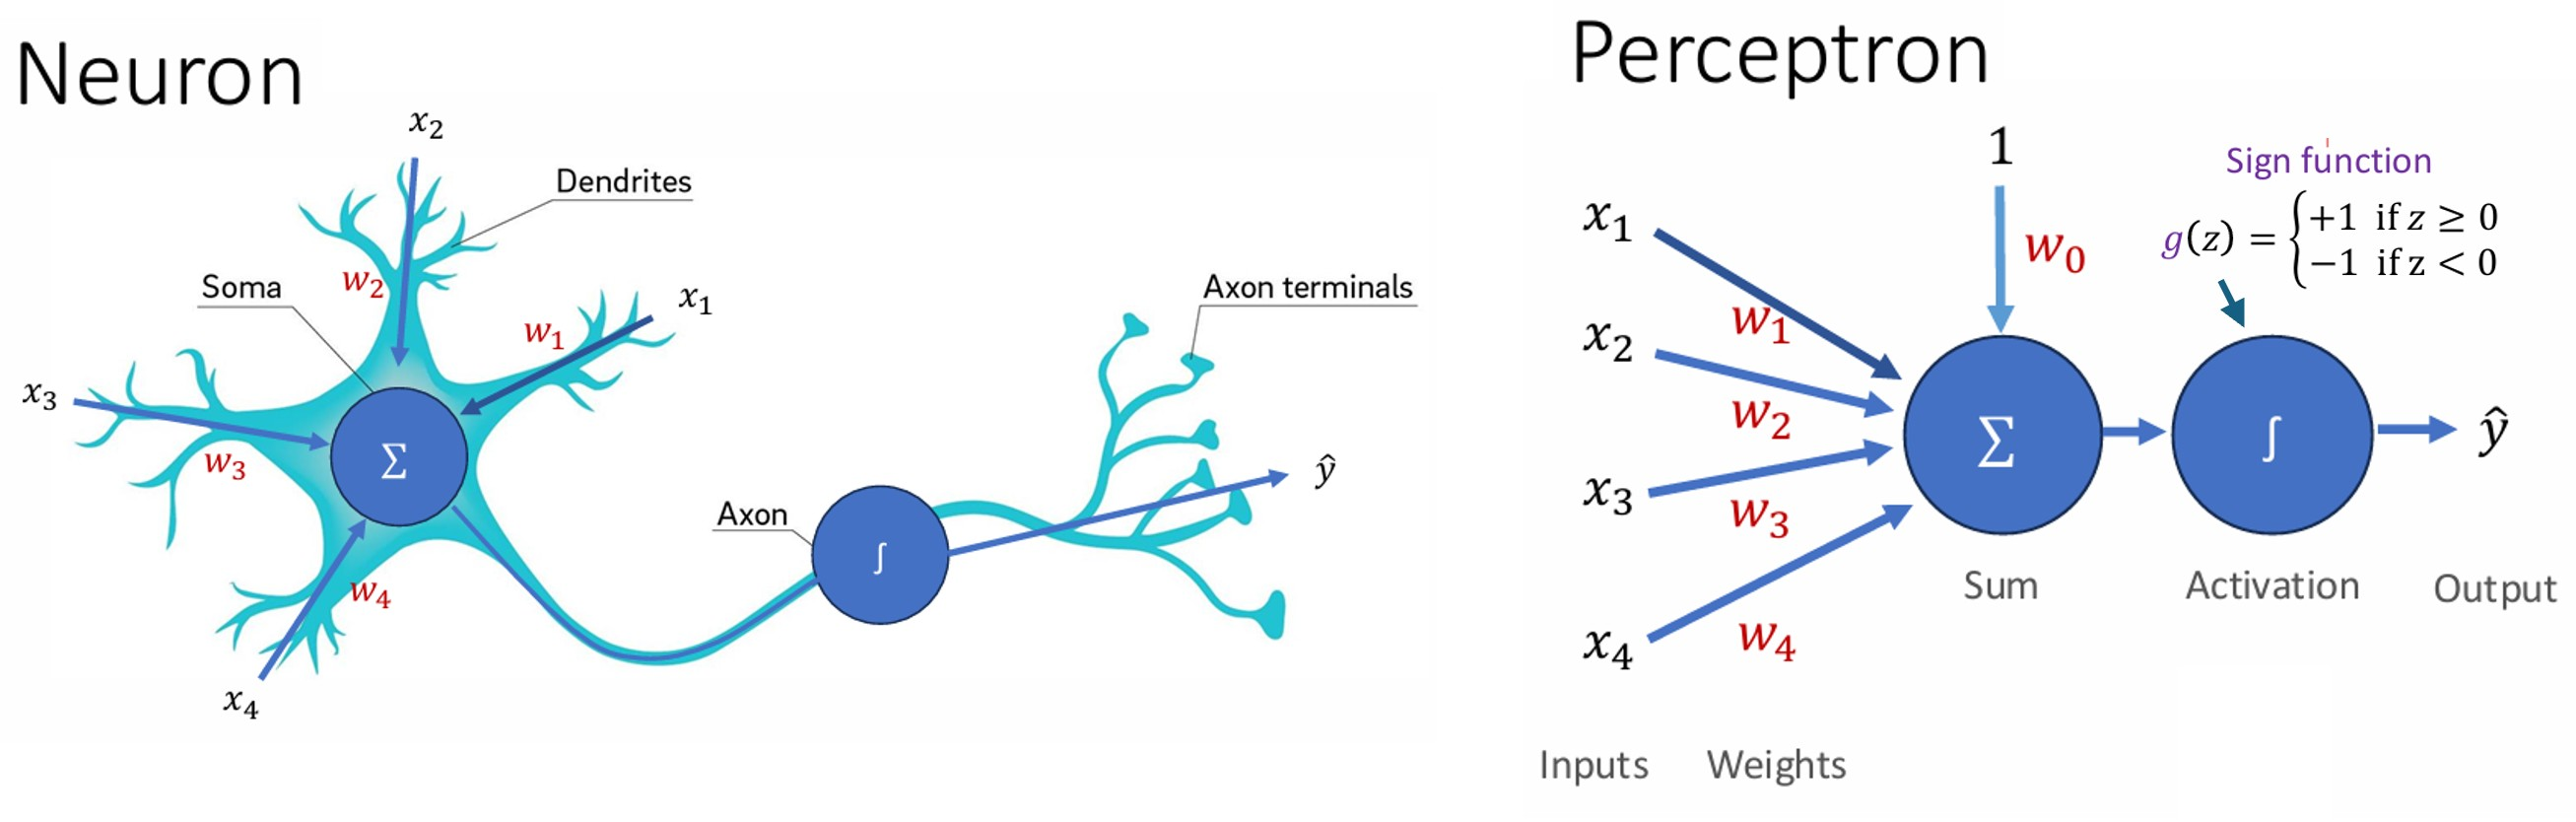
\includegraphics[width=1\linewidth]{perceptron}}

\subsubsection{Perceptron Model}
Given an input vector $\mathbf{x}$ of dimension $d$, the perceptron model is defined as:
\[
h_w(x) = \hat{y} = g(\mathbf{w}^T \mathbf{x}) = g\left(\sum_{j=0}^d w_j x_j\right), \quad g(z) =
\begin{cases}
+1 & \text{if } z \geq 0, \\
-1 & \text{if } z < 0.
\end{cases}
\]
\begin{itemize}[itemsep=0pt]
\item $h_w(x) = g(w_0x_0 + w_1x_1 + ... + w_dx_d)$
\item $\mathbf{w} = [w_0, w_1, \dots, w_d]$ are the weights (parameters) of the perceptron.
\item $x_0 = 1$ is a dummy variable (bias term).
\item $g(z)$ is the activation function, typically a step function.
\item $N$ \textbf{data points}, each has \textbf{Features}: $x^{(i)} \in \mathbb{R}^d$ \quad \textbf{Target}: $y^{(i)} \in {-1, 1}$
\item Features are described by a vector of real numbers in dimension $d$ (i.e. $x$)
\end{itemize}

\subsubsection{Perceptron Learning Algorithm}
The perceptron learning algorithm is used to train the model by iteratively updating the weights to minimize misclassifications:
\begin{enumerate}[itemsep=0pt]
    \item Initialize the weights $\mathbf{w}$ (e.g., to zero or small random values).
    \item For each training instance $(\mathbf{x}^{(i)}, y^{(i)})$: 
    \begin{itemize}[topsep=0pt]
		\item Compute predicted output $\hat{y}^{(i)} = g(\mathbf{w}^T \mathbf{x}^{(i)})$
		\item If prediction incorrect ($\hat{y}^{(i)} \neq y^{(i)}$), i.e. misclassified, update weights:\\
		$[\mathbf{w} \leftarrow \mathbf{w} + \gamma \cdot (y^{(i)} - \hat{y}^{(i)}) \cdot \mathbf{x}^{(i)}]$, 
		        where $\gamma$ is the learning rate.
	\end{itemize}
    \item Repeat until convergence or a maximum number of iterations is reached.
\end{enumerate}
\textbf{Example: Cancer Prediction}: Binary classification problem, goal to predict whether tumor benign ($-1$) or malignant ($+1$) based on size. 

\centerline{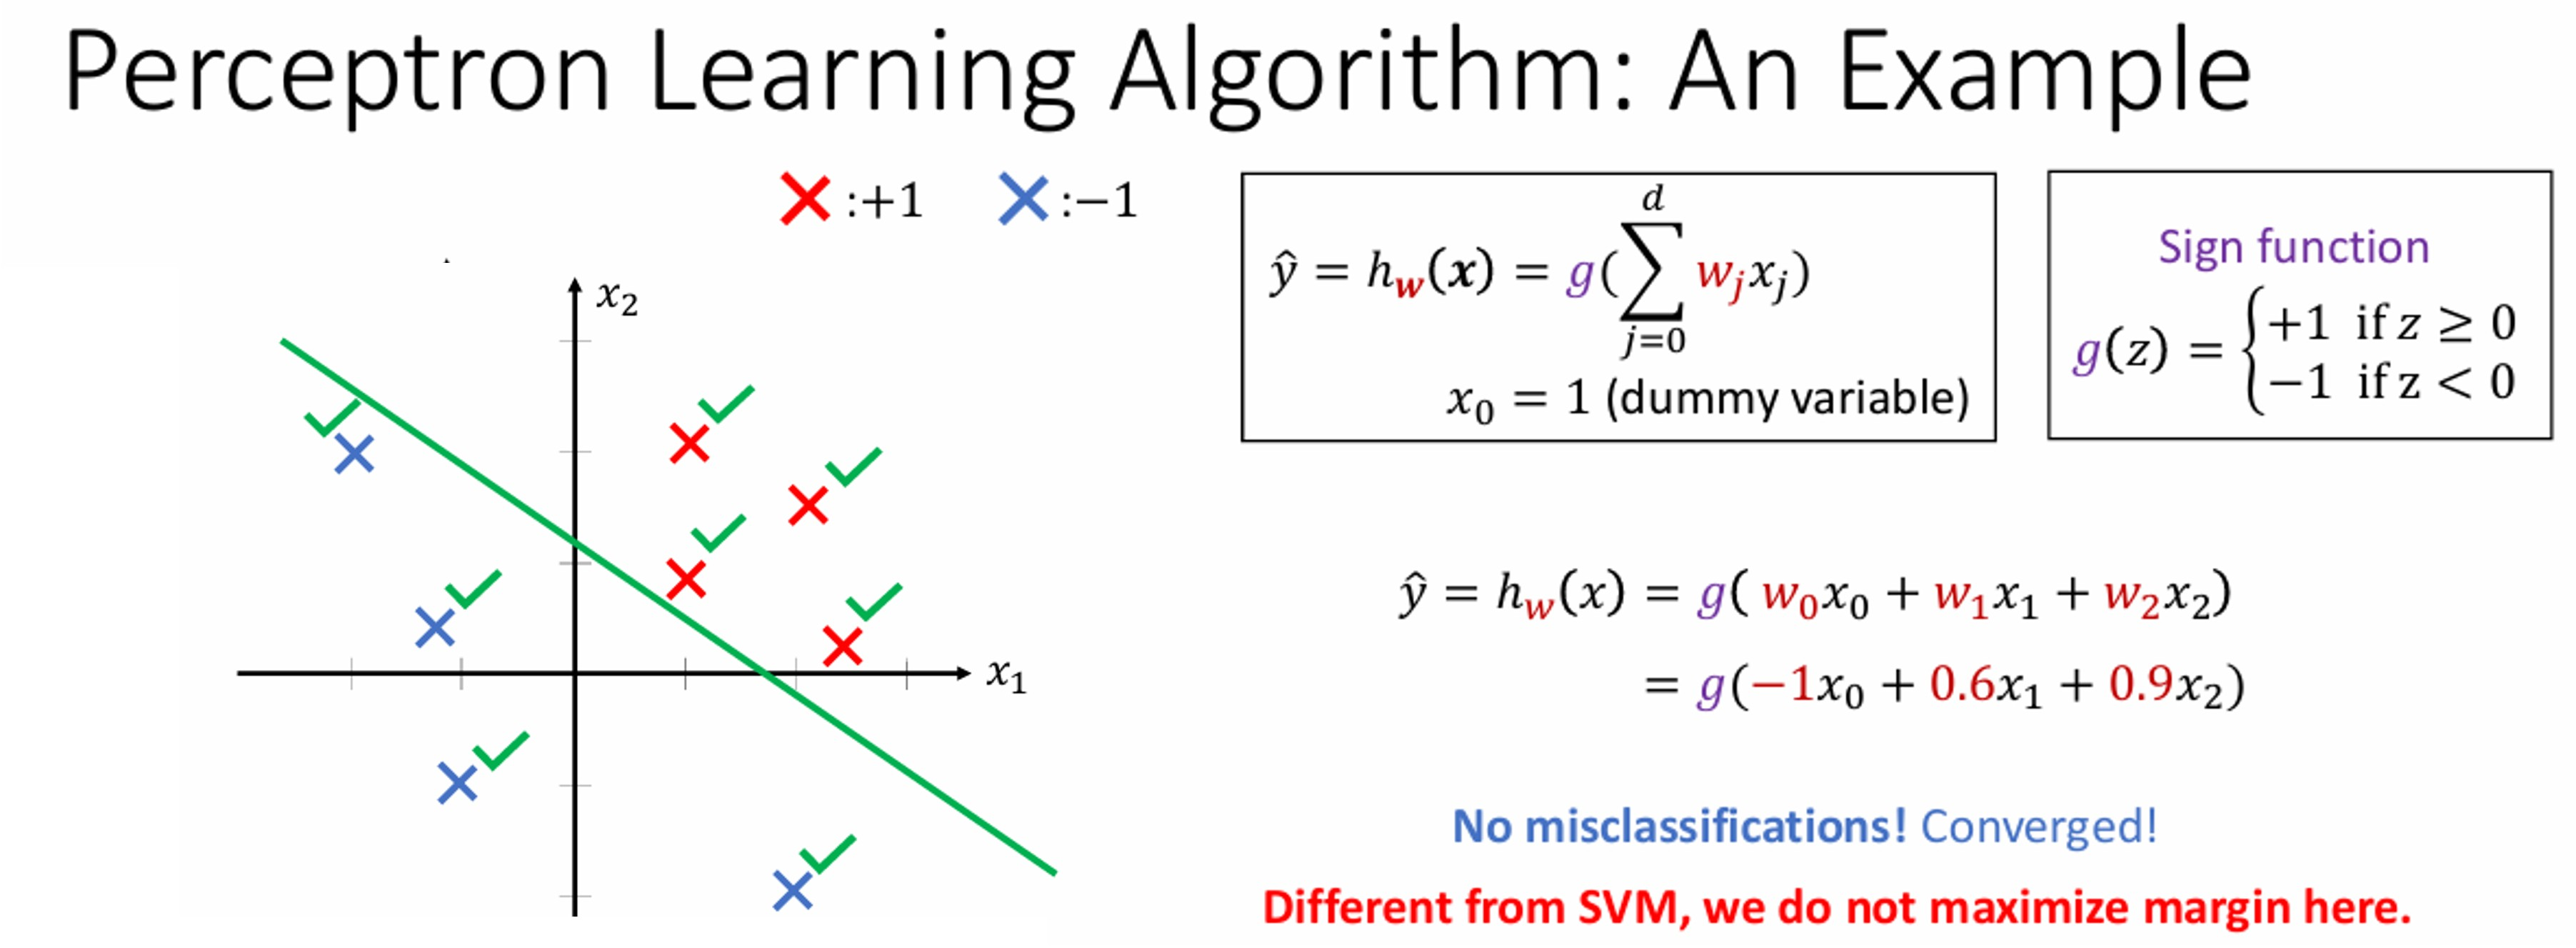
\includegraphics[width=0.9\linewidth]{perceptronLearning}}

\subsubsection{Limitations of the Perceptron}
\begin{itemize}
\item It can only solve linearly separable problems.
\item It does not handle non-linear relationships between features.
\item To address these limitations, multi-layer neural networks are used, which stack multiple perceptrons (neurons) with non-linear activation functions.
\end{itemize}

% ---------- 

\subsection{Neural Network}
A neural network is composed of multiple layers of interconnected neurons, enabling it to learn complex patterns in data.

\subsubsection{Neuron}
An artificial neuron generalizes perceptron using diff. activation functions: \\

\centerline{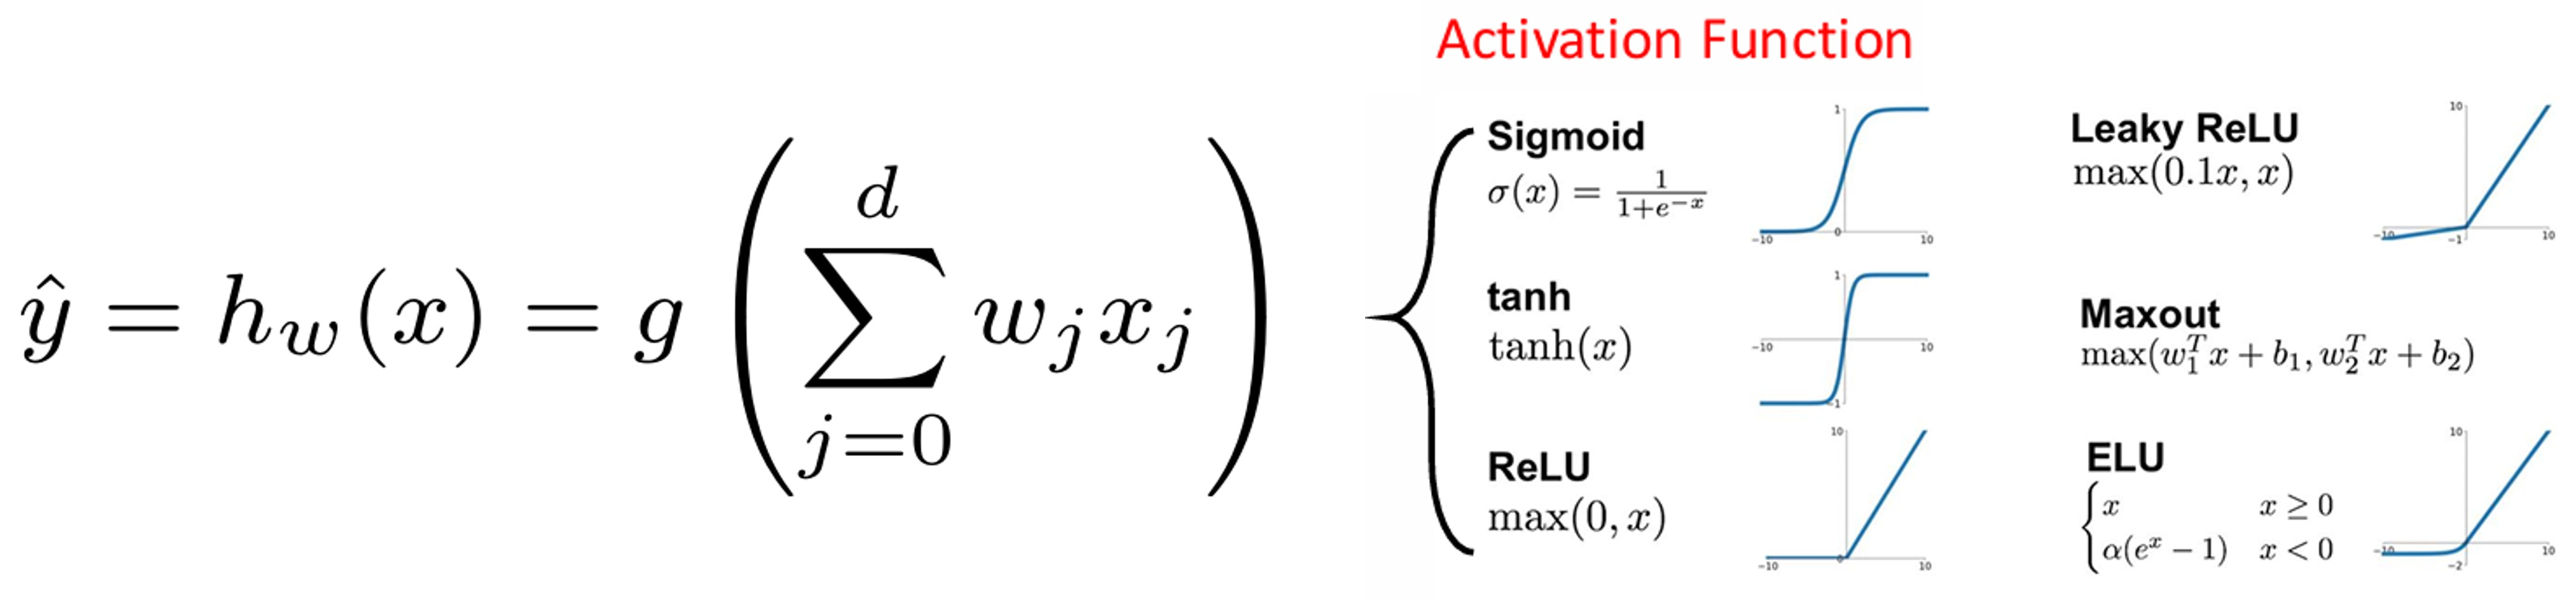
\includegraphics[width=0.9\linewidth]{neuronFormula}}
%\[
%\hat{y} = h_w(x) = g\left(\sum_{j=0}^d w_j x_j\right)
%\]
(activation function $g(z)$ e.g. ReLu, sigmoid function: $g(z) = \frac{1}{1 + e^{-z}}$)
\begin{itemize}[itemsep=0pt]
\item A neuron w. linear activation function equivalent to linear regression model.
\item A neuron w. sigmoid activation function eqv to logistic regression model.
	\begin{itemize}[itemsep=0pt, topsep=0pt]
	\item Identity/Linear activation fn: $g(z) = z \implies h_w(x) = \sum_{j=0}^d w_j x_j$
	\item Sigmoid function: $g(z) = \sigma(z) \implies h_w(x) = \sigma(\sum_{j=0}^d w_j x_j)$
	\end{itemize}
\end{itemize}

\subsection{Feature Engineering for Non-Linear Problems}
To model non-linearly separable problems (e.g., XNOR gate), feature engineering is essential. Two approaches are commonly used:
\begin{itemize}
\item \textbf{Manual Feature Engineering}: Manual transform existing features to capture non-linear relationships, e.g. polynomial features: $x_1^2, x_2^2, x_1x_2$, apply exponential or logarithmic transformations: $e^{x_1}, \log(x_2)$, combine features multiplicatively: $x_1x_2$. 
\item \textbf{Using Neurons for Feature Transformation}: Instead of manual transforms, use neurons in neural network to automatically learn new features. Hidden layers apply non-linear activation functions (e.g., sigmoid, ReLU). Weights of neurons effectively create new features making it linearly separable.
\end{itemize}

\centerline{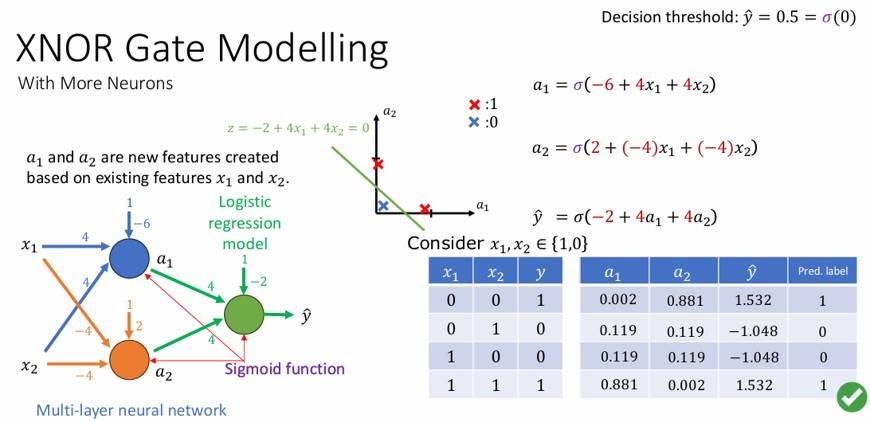
\includegraphics[width=1\linewidth]{XNOR}}
\begin{itemize}
\item Linear Regression and Logisitic Regression relies on manual feature engineering to capture complex patterns, while a multi-layer neural network learns its own feature representations through its layers with activation functions.
\end{itemize}

\subsubsection{Multi-layer Neural Networks}

Multi-layer neural networks consist of an \textbf{input layer} (receives raw features), \textbf{hidden layers} (transform features using learned weights and activation functions), an \textbf{output layer} (produces final predictions).

\centerline{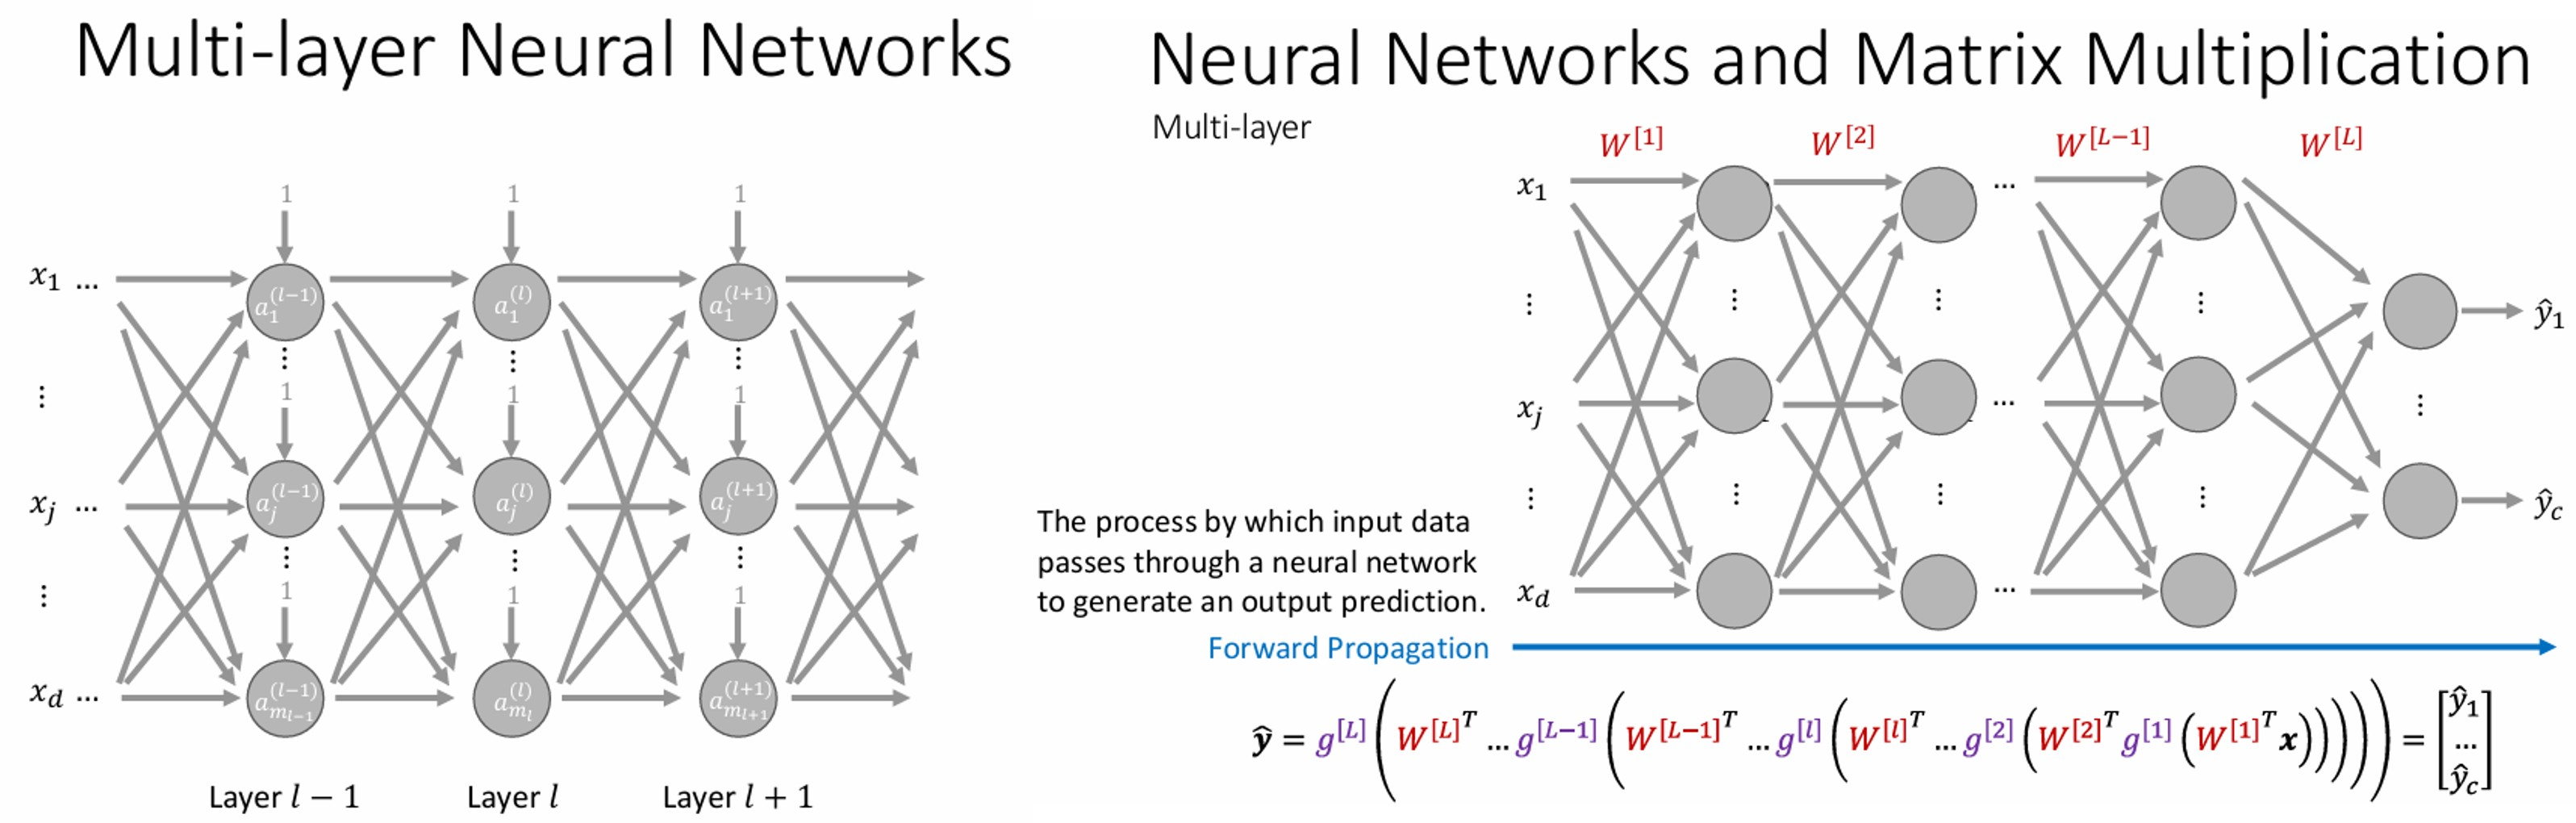
\includegraphics[width=1\linewidth]{multiLayerNeuralNetworks}}

The forward propagation process computes the output as:
\[
\hat{\mathbf{y}} = g^{[L]} \left( W^{[L]} \cdot g^{[L-1]} \left( W^{[L-1]} \cdot \dots g^{[1]} \left( W^{[1]} \cdot \mathbf{x} \right) \dots \right) \right),
\]
where $W^{[l]}$ are the weights for layer $l$, and $g^{[l]}$ is the activation function.

\subsubsection{Softmax Activation for Multi-class Classification}
For multi-class classification, the softmax function is used in the output layer to convert raw scores into probabilities:
\[
g(z_i) = \frac{e^{z_i}}{\sum_{j=1}^c e^{z_j}},
\]
where $c$ is the number of classes, and $g(z_1) + g(z_2) + \dots + g(z_c) = 1$.

\smallskip

\centerline{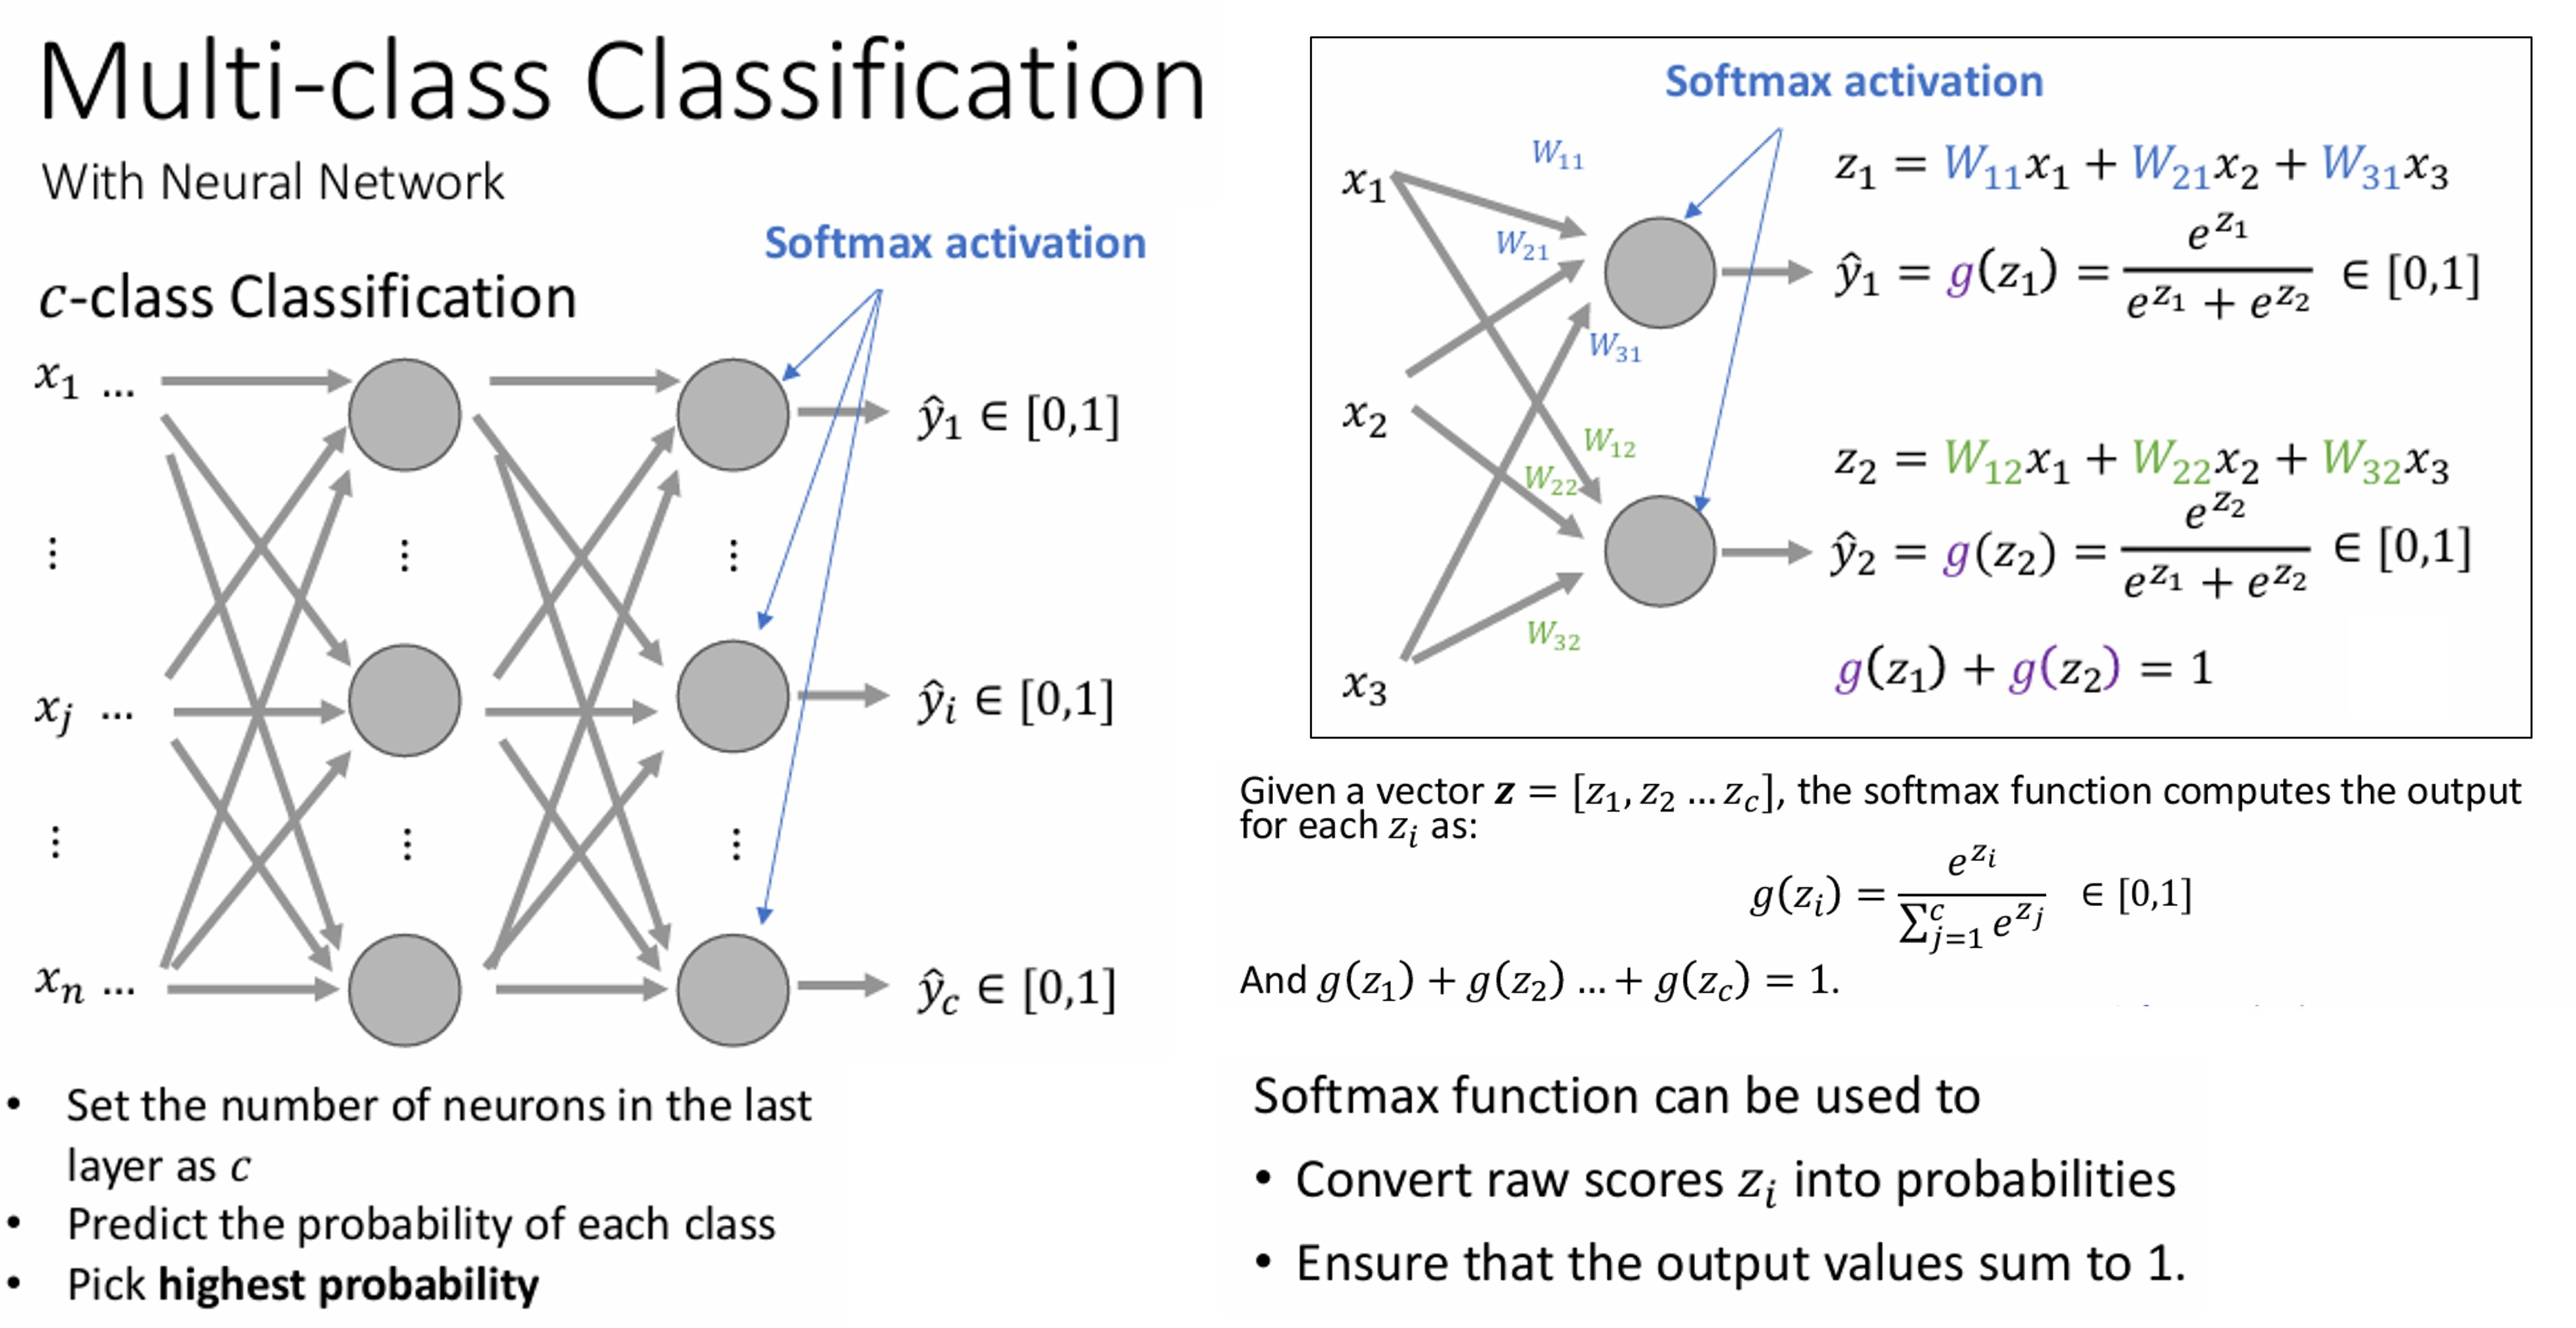
\includegraphics[width=1\linewidth]{neuralMulticlass}}

\subsubsection{Summary}
\begin{itemize}
\item \textbf{Applications}: Neural networks widely used for image classification, (identifying objects in images), natural language processing (sentiment analysis), multi-class classification (predicting one of several categories).
\item \textbf{Perceptron} is a single-layer binary classifier.
\item Neural networks generalize the perceptron by stacking multiple layers and using non-linear activation functions.
\item Multi-layer neural networks models complex, non-linear data relationships.
\end{itemize}

\subsection{Neural Networks Training}

Training a neural network involves adjusting its weights to minimize loss function, measures difference between predicted output and true target values. Gradient descent usable to update weights in neural network. 

\centerline{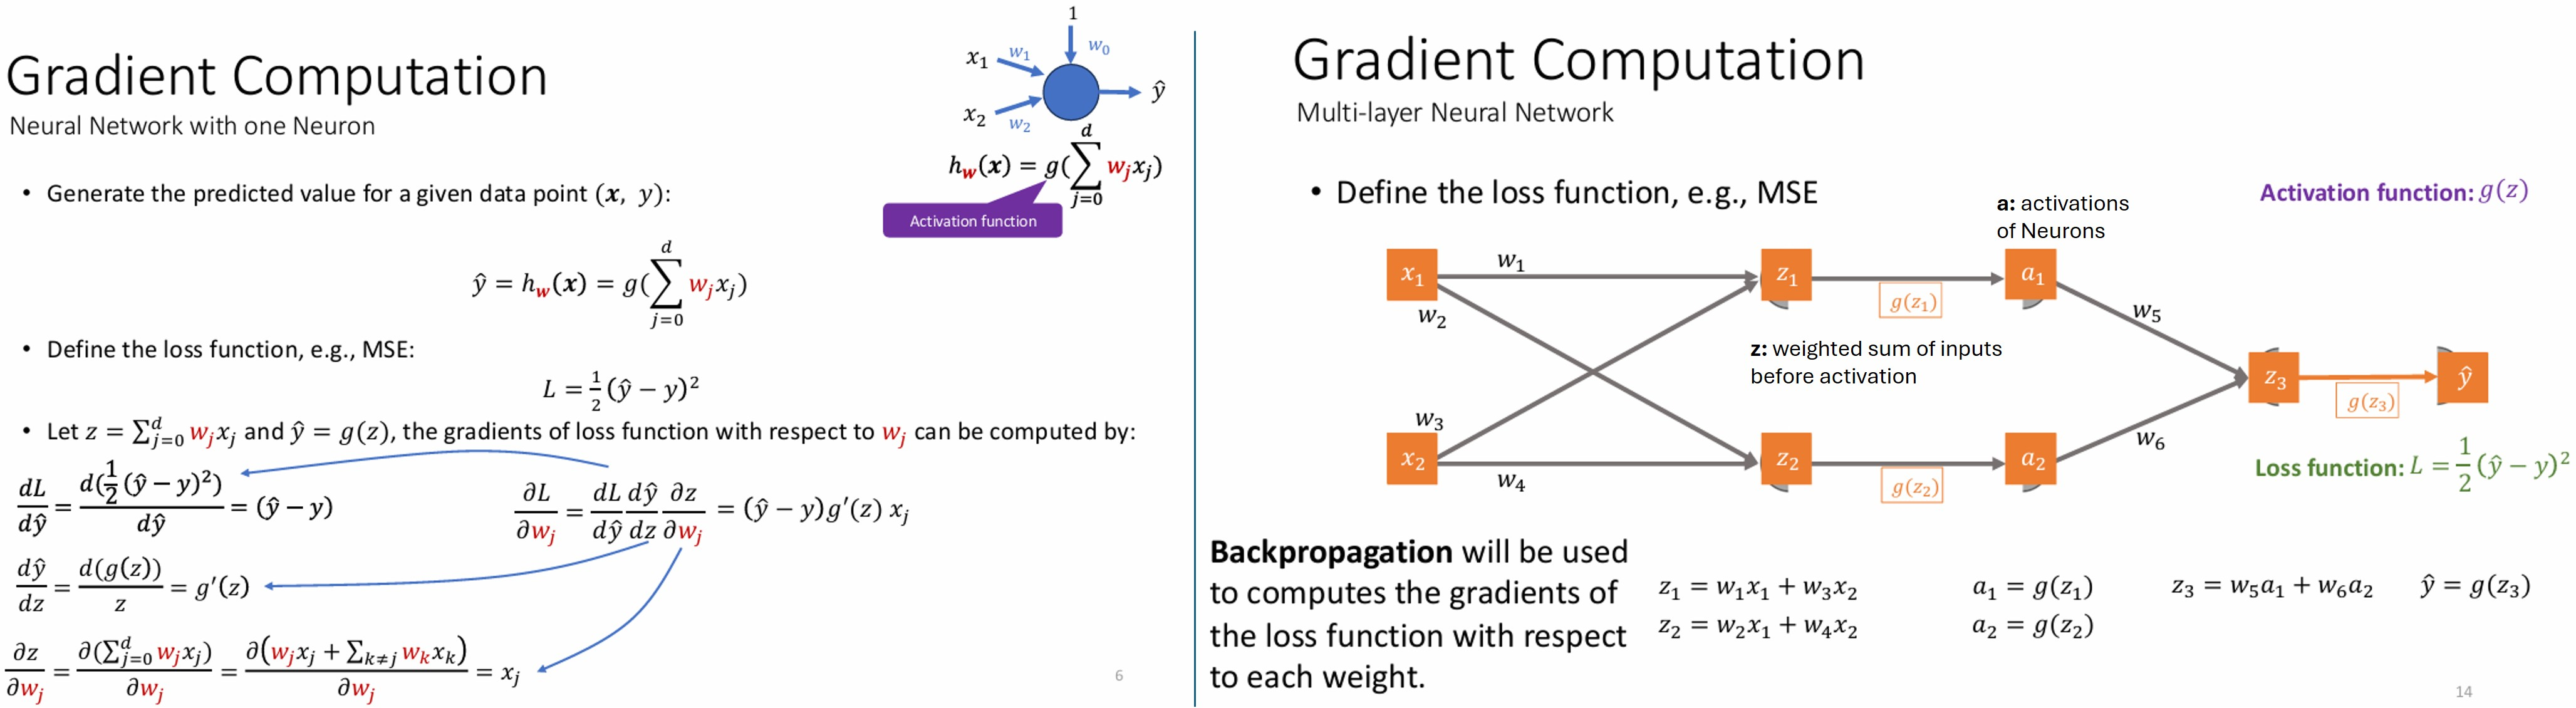
\includegraphics[width=1\linewidth]{multiLayer2}}
\smallskip
\centerline{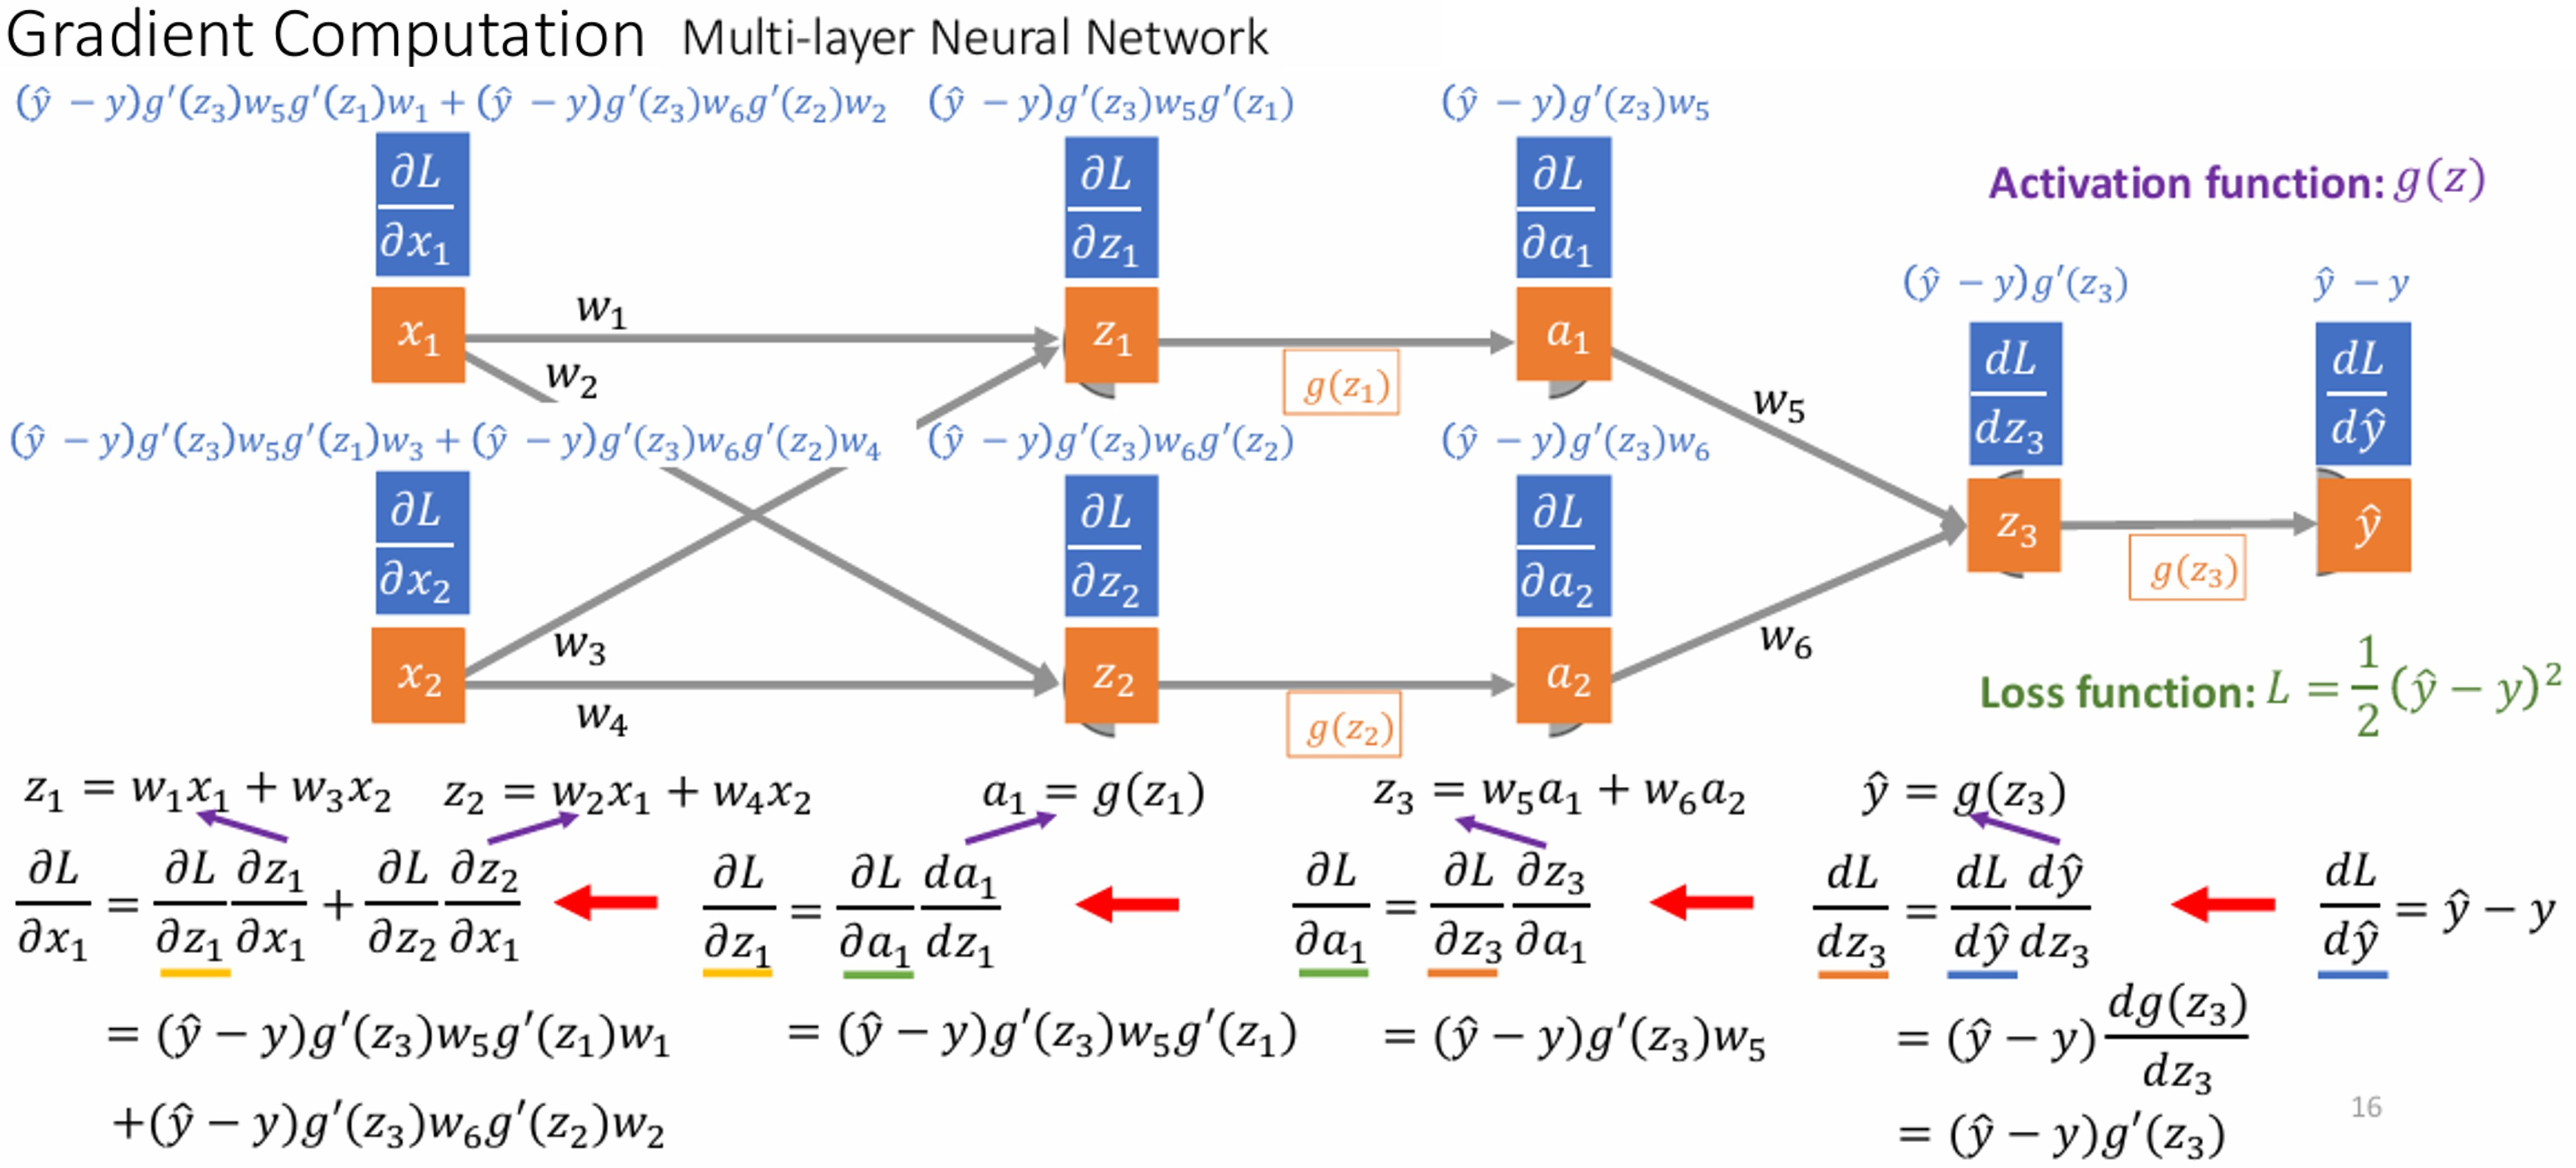
\includegraphics[width=1\linewidth]{multiLayer3}}

\subsubsection{Forward Propagation}
During forward propagation, input data is passed through the network layer by layer to compute the predicted output:
\begin{itemize}[itemsep=0pt]
\item $\hat{y} = g(W^{[L]} \cdot g(W^{[L-1]} \cdot \dots g(W^{[1]} \cdot x) \dots ))$
\item $ W^{[l]} $: Weight matrix for layer $ l $, $ x $: Input features.
\item $ g(\cdot) $: Activation function (e.g., ReLU, sigmoid, softmax).
\item For example, in a simple multi-layer neural network:
\end{itemize}
\centerline{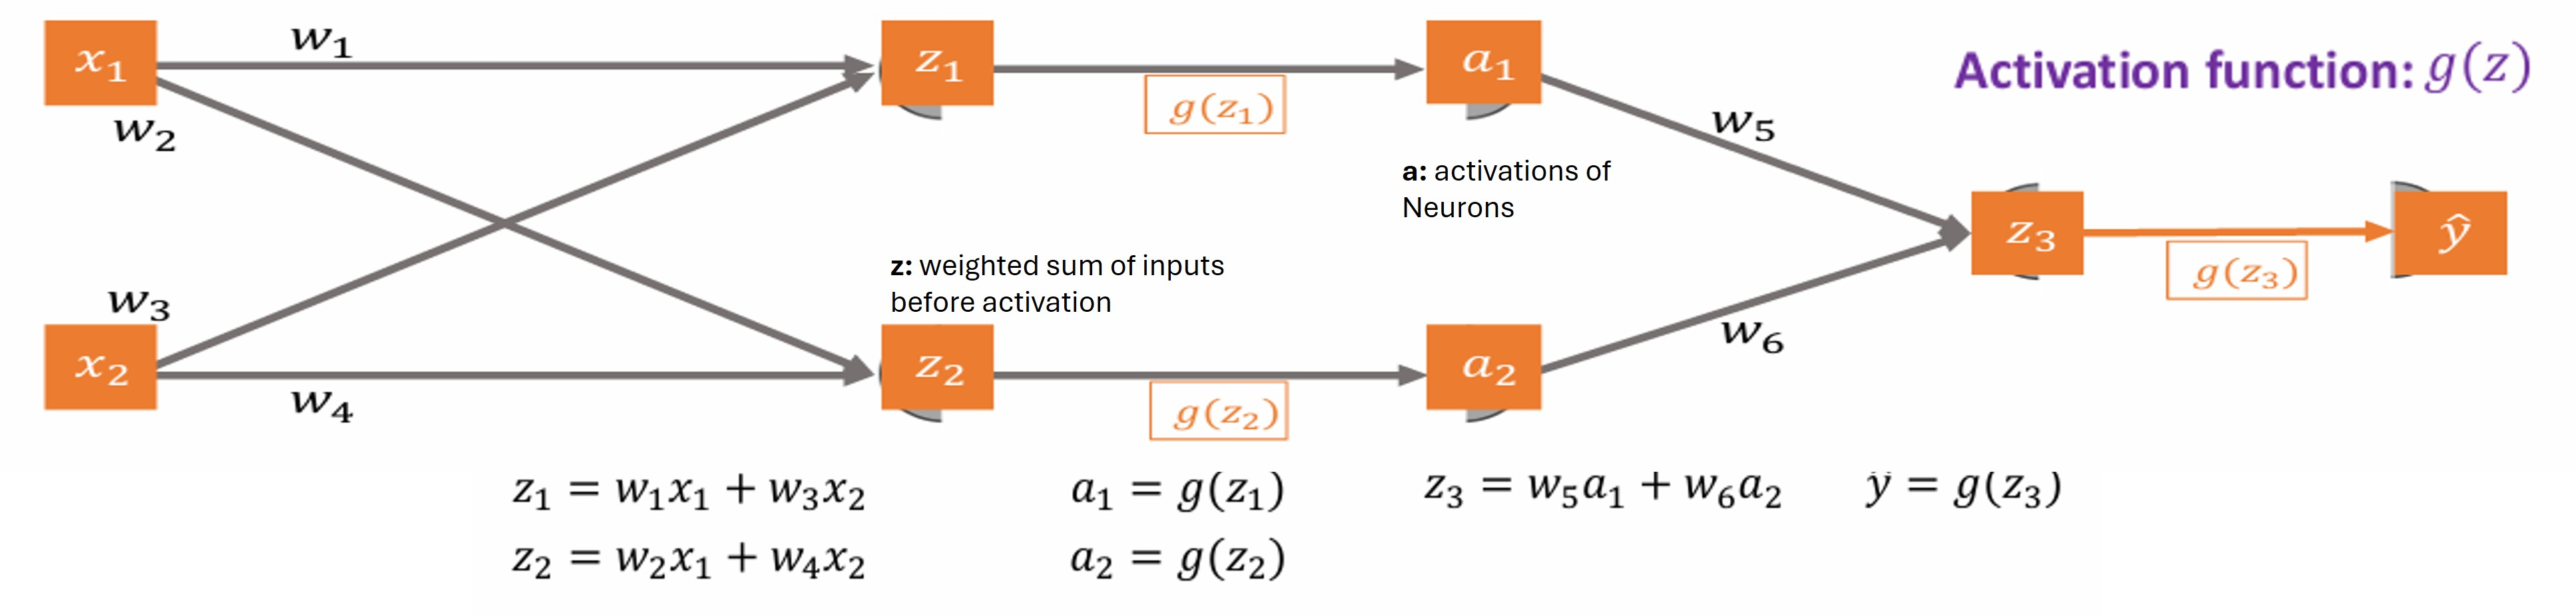
\includegraphics[width=1\linewidth]{forwardPropagation}}


\textbf{Loss Function}: quantifies error between predicted output $ \hat{y} $ and the true target $ y $. Common loss functions include Mean Squared Error (MSE) 
($L = \frac{1}{2} (\hat{y} - y)^2$), Cross-Entropy Loss (for classification tasks).


\subsubsection{Backpropagation}
Compute gradients of loss function w.r.t weight w. chain rule (MSE Loss):
$$
\frac{\partial L}{\partial w_j} = \frac{\partial L}{\partial \hat{y}} \cdot \frac{\partial \hat{y}}{\partial z} \cdot \frac{\partial z}{\partial w_j}.
\quad \leftrightarrow \frac{\partial L}{\partial \hat{y}} = \hat{y} - y. \quad \frac{\partial \hat{y}}{\partial z} = g'(z).  \quad \frac{\partial z}{\partial w_j} = x_j.
$$
\begin{itemize}[itemsep=0pt]
\item $L = \frac{1}{2} (\hat{y} - y)^2$, so $\frac{\partial L}{\partial \hat{y}} = \hat{y} - y$, and $\quad$ $\hat{y} = g(z)$, so $\frac{\partial \hat{y}}{\partial z} = g'(z).$
\item e.g. $z_1 = w_1x_1 + w_3x_2$, so: $\frac{\partial z_1}{\partial w_i} = x_j$
\end{itemize}
\textbf{Key steps in backpropagation}: Compute derivative of loss wrt. output y. Compute derivative of activation function. Propagate error backward through layers, compute respective derivatives. Then compute gradients $\forall$ weights. \\
\smallskip
\centerline{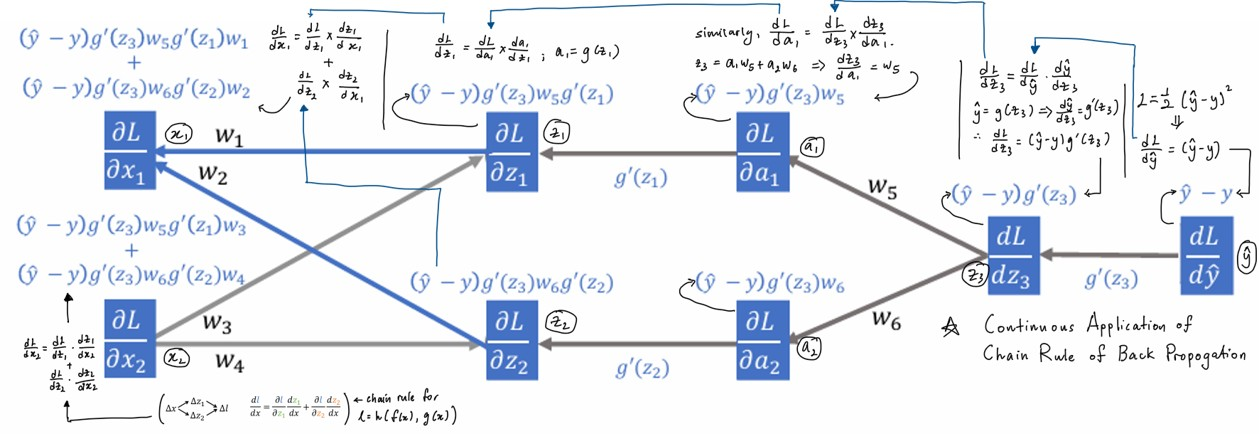
\includegraphics[width=1\linewidth]{backPropagation}}
\subsubsection{Gradient Computation}
\centerline{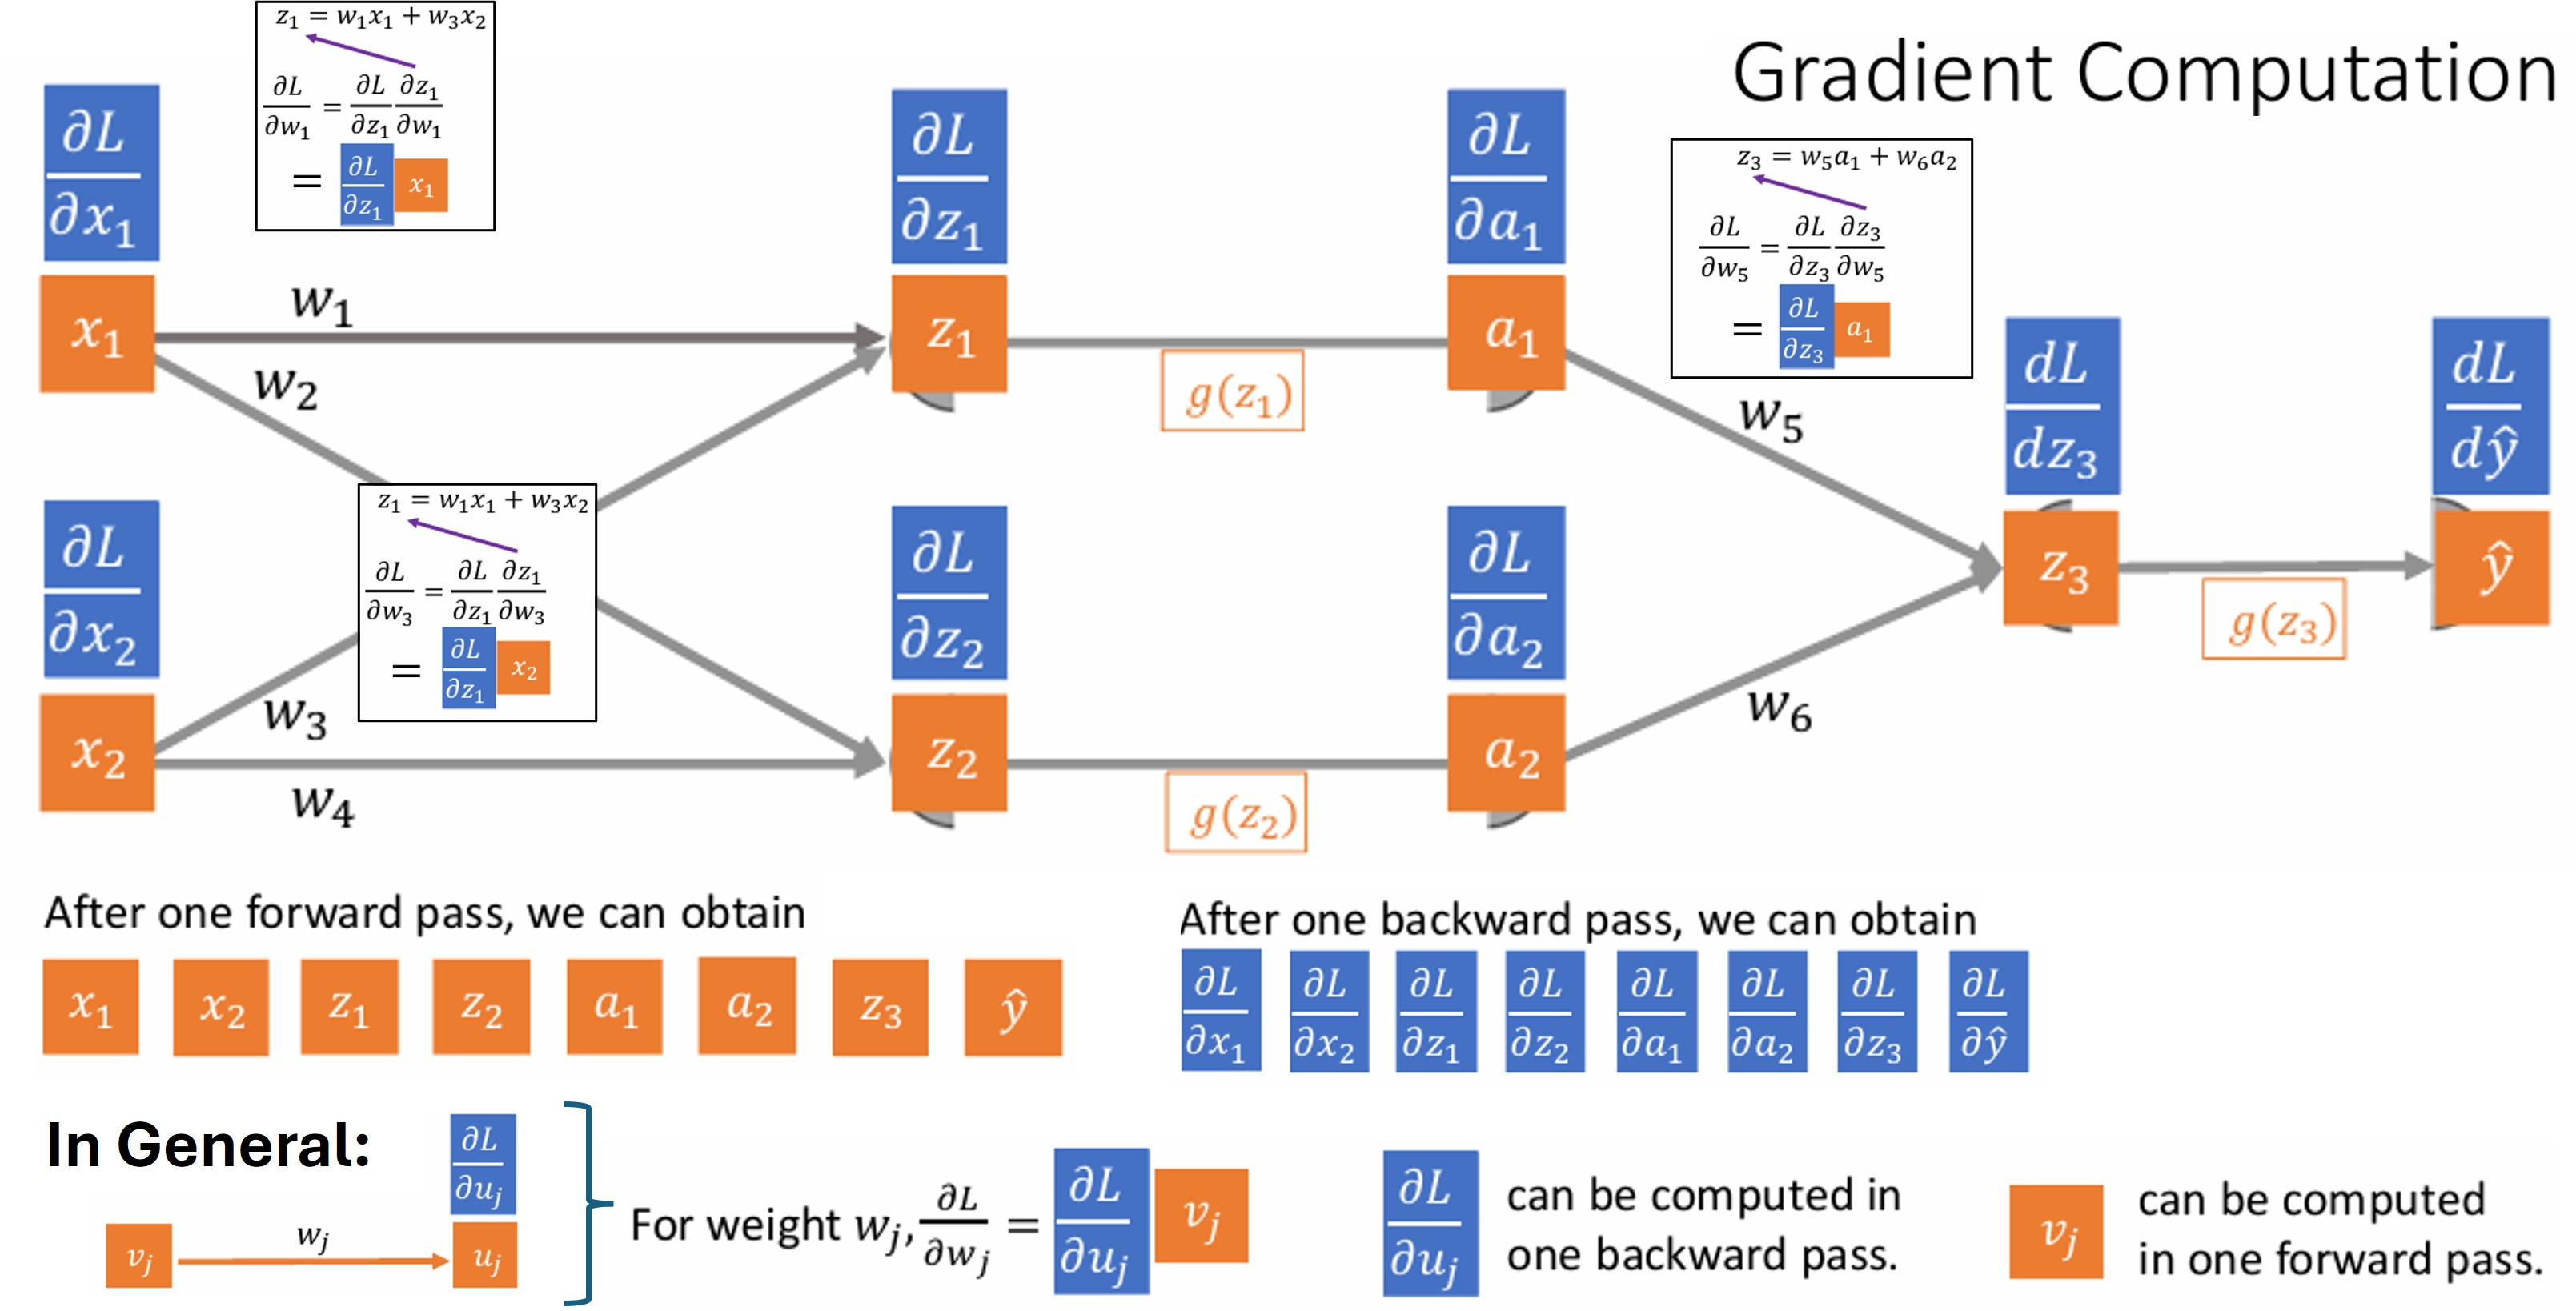
\includegraphics[width=1\linewidth]{gradientComputation}}
E.g. gradient of loss w.r.t $ w_3 $ in the above simple network: 
$\frac{\partial L}{\partial w_3} =  \frac{\partial L}{\partial z_1} \cdot \frac{\partial z_1}{\partial w_3} = [ (\hat{y} - y) \cdot g'(z_3) \cdot w_5 \cdot g'(z_1) ] \cdot [ x_2 ]$

\columnbreak

\subsubsection{Gradient Descent}
 Once gradients are computed, weights updated using gradient descent:
$$
w_j \leftarrow w_j - \gamma \frac{\partial L}{\partial w_j}, \quad \gamma : \text{ learning rate.}
$$


\subsubsection{Iterative Optimization}
The forward propagation, loss computation, backpropagation, and weight update steps are repeated iteratively until convergence / stopping criterion.

\subsection{Neural Network with One Neuron}
A single neuron is the simplest form of a neural network. It performs the following operations:
\begin{enumerate}[itemsep=0pt, topsep=0pt]
    \item \textbf{Weighted Sum}: $z = \sum_{j=0}^d w_j x_j = w^T x$, ($ w_0 $: bias term).
    \item \textbf{Activation Function}: $\hat{y} = g(z)$, e.g. sigmoid fn: $g(z) = \frac{1}{1 + e^{-z}}$
\end{enumerate}
\begin{itemize}[itemsep=0pt, topsep=0pt]
\item For binary classification, activation function is typically sigmoid function.
\item The loss function for a single neuron is often the binary cross-entropy loss: $L = -y \log(\hat{y}) - (1-y) \log(1-\hat{y}).$
\end{itemize}
\subsection{Multi-layer Neural Network}
A multi-layer neural network consists of multiple layers of neurons, enabling it to model complex, non-linear relationships. Key components include:




%% ADD TUTORIAL NOTES HERE %
\subsubsection{Hidden Layers}
Hidden layers transform the input features into higher-level representations:
$$
a^{[l]} = g(W^{[l]} a^{[l-1]} + b^{[l]}),
$$
where $ a^{[l]} $ is the activation of layer $ l $.

\subsubsection{Activation Functions}
Common activation functions include:

    
- ReLU (Rectified Linear Unit): $ g(z) = \max(0, z) $.
    
- Sigmoid: $ g(z) = \frac{1}{1 + e^{-z}} $.
    
- Softmax (for multi-class classification):
    $$
    g(z_i) = \frac{e^{z_i}}{\sum_{j=1}^c e^{z_j}}.
    $$


\subsubsection{Output Layer}
The output layer produces the final prediction. For regression tasks, it uses a linear activation function. For classification tasks, it uses softmax or sigmoid.


%% UP TILL HERE
\vfill \null
\columnbreak


\subsection{Introduction to PyTorch}
PyTorch: popular deep learning library, simplifies implementation of neural networks. Flexible, efficient framework for building, training models.

\subsubsection{Modules and Functions API}
PyTorch organizes neural network components into modular containers and layers. Key components include:
\begin{itemize}
\item \textbf{Containers}:
\begin{itemize}
\item \texttt{torch.nn.Module}: Base class for all neural network modules.
\item \texttt{torch.nn.Sequential}: A container for stacking layers sequentially.
\end{itemize}
\item \textbf{Linear Layers}:
	\begin{itemize}
	\item \texttt{torch.nn.Linear}: A fully connected layer without activation.
	\end{itemize}
\item \textbf{Non-linear Activation Functions}:
	\begin{itemize}
	\item \texttt{torch.nn.ReLU}: Rectified Linear Unit.
	\item \texttt{torch.nn.Sigmoid}: Sigmoid activation function.
	\item \texttt{torch.nn.Softmax}: Softmax activation function (commonly used for multi-class classification).
	\end{itemize}
\item \textbf{Loss Functions}: Various for diff. tasks:
	\begin{itemize}
	\item \texttt{torch.nn.MSELoss}: Mean Squared Error (MSE) for regression tasks.
	\item \texttt{torch.nn.BCELoss}: Binary Cross Entropy Loss, binary classification.
	\item \texttt{torch.nn.CrossEntropyLoss}: Cross-Entropy Loss, multi-class classification.
	\end{itemize}
\item \textbf{Optimizers}: (update weights during training)
	\begin{itemize}
	\item Stochastic Gradient Descent (SGD): \texttt{torch.optim.SGD}.
	\item Adam: \texttt{torch.optim.Adam}.
	\item \textbf{Important optimizer functions}: \\
	 \texttt{optimizer.zero\_grad()}: Resets gradients to zero before computing new gradients.\\
	  \texttt{optimizer.step()}: Updates the weights after backpropagation.
	\end{itemize}
\end{itemize}

\subsubsection{Building a Neural Network Example}
\centerline{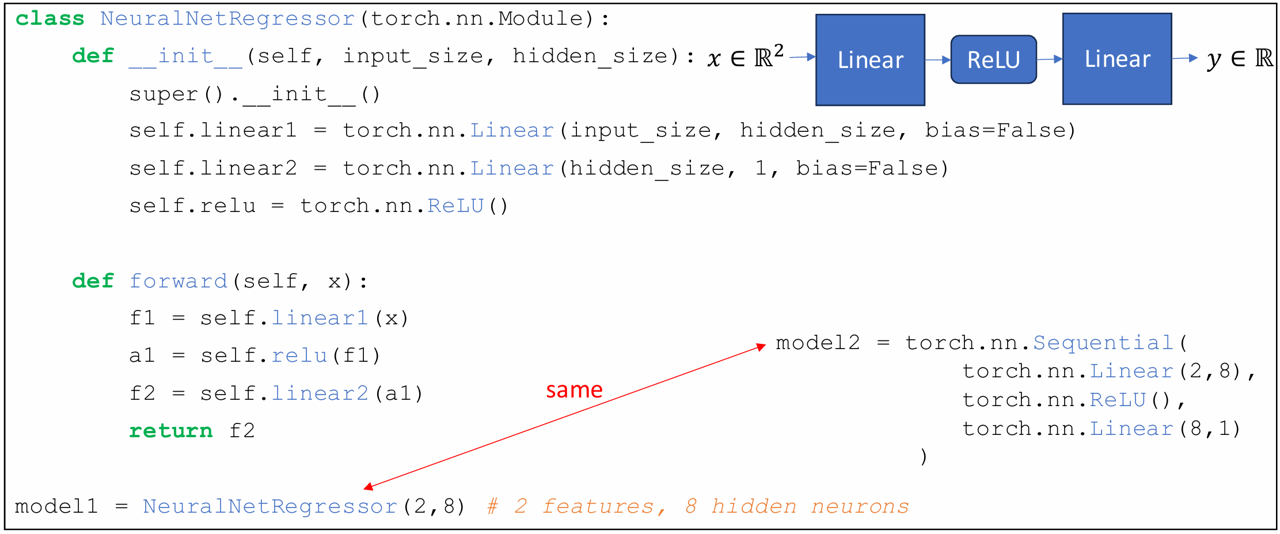
\includegraphics[width=1\linewidth]{pytorch}}
\subsubsection{Training a Neural Network Example}
\centerline{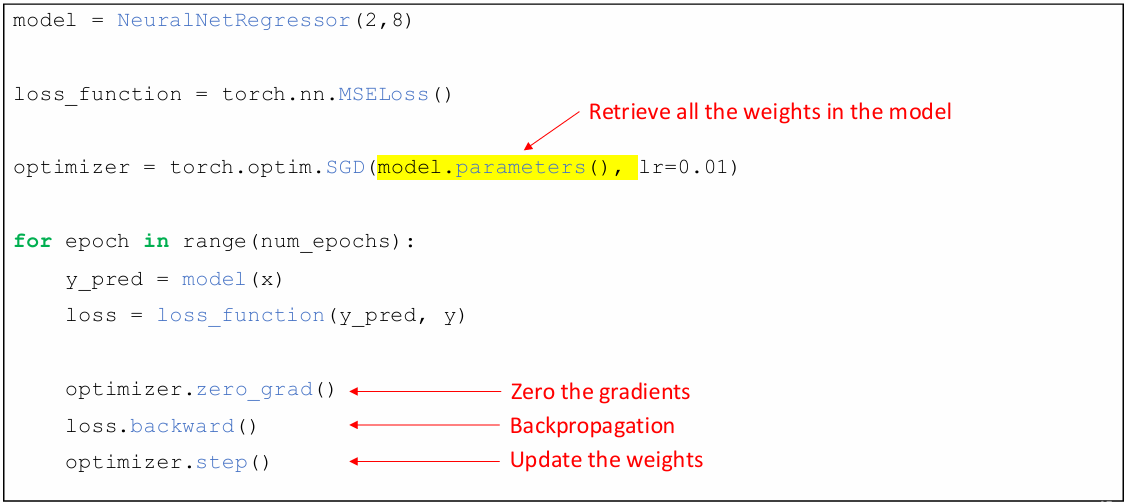
\includegraphics[width=1\linewidth]{pytorch2}}

\columnbreak

\subsection{12. \underline{Convolutional Neural Networks (CNNs)}}
CNNs: specialized neural networks for process grid-like data (e.g. image).
\begin{itemize}
\item Leverage convolution operations to extract spatial features efficiently.
\item \textbf{Convolution} is a mathematical operation that combines two functions to produce a third function. In context of CNNs:
	\begin{itemize}
	\item One function represents the input data (e.g., an image).
	\item Other function represents a small matrix called a filter or kernel
	\item The convolution operation involves sliding the filter over the input and computing the weighted sum at each position. This process extracts spatial features from the input, such as edges, textures, or patterns.
	\end{itemize}
\end{itemize}


\subsubsection{Convolution Layer}
Applies filters to extract spatial features: $\text{Output} = \text{Input} * \text{Filter} + \text{Bias}.$
\begin{itemize}
\item \textbf{PyTorch}: {\tiny \texttt{conv\_layer = nn.Conv2d(in\_channels, out\_channels, kernel\_size, stride, padding)}}
\end{itemize}
\centerline{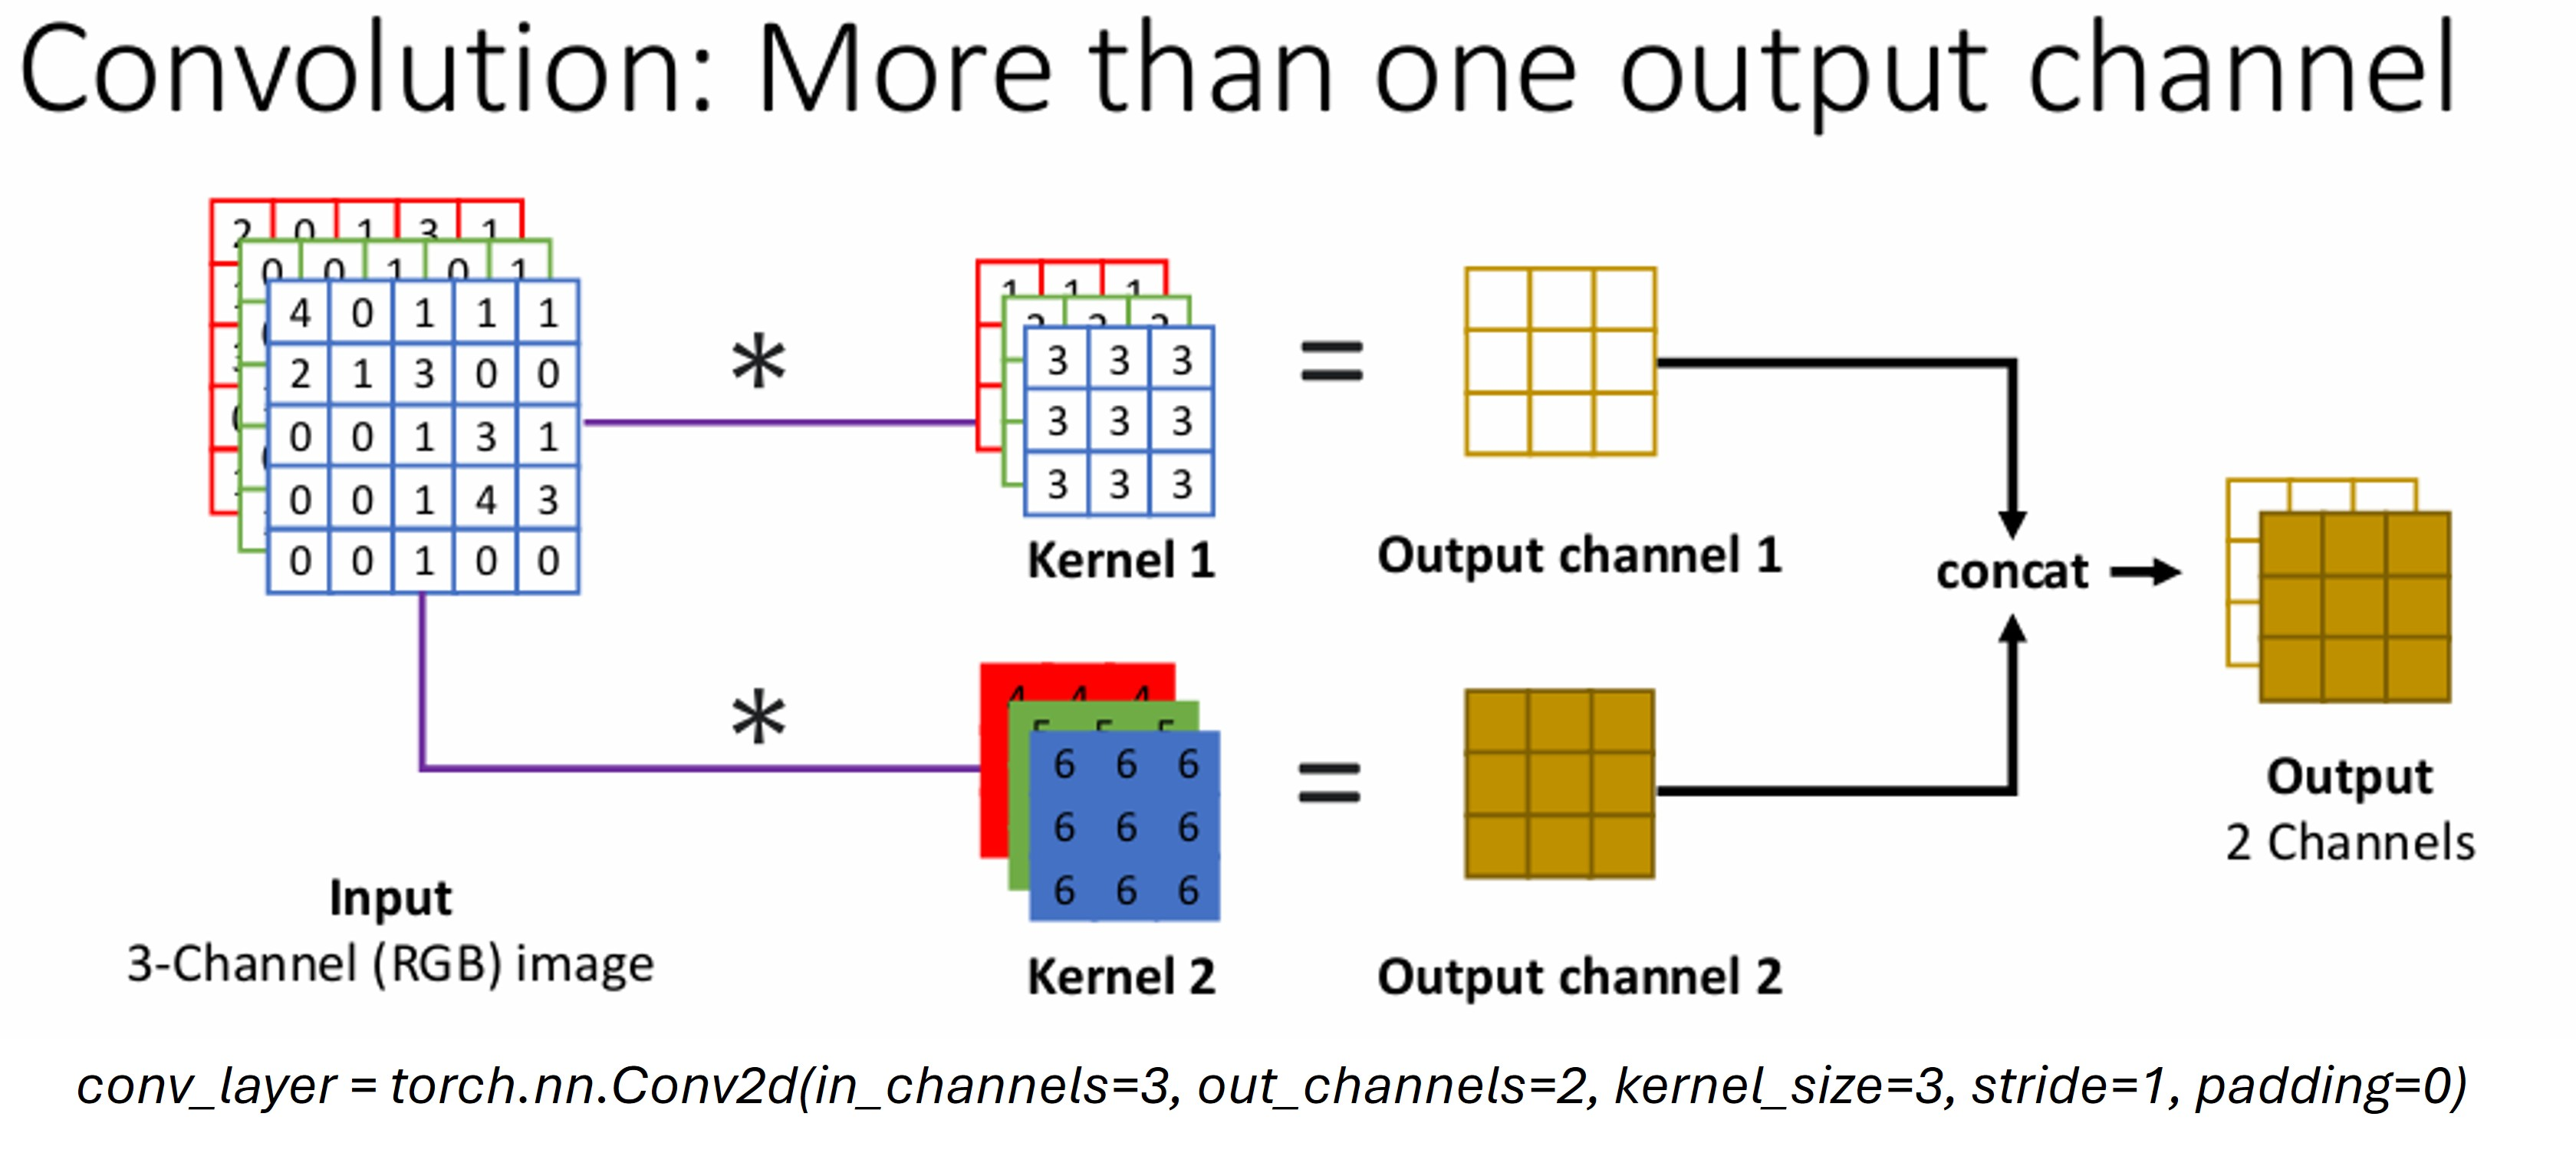
\includegraphics[width=0.8\linewidth]{convoLayer}}

\textbf{Example of Convolution Operation}: Consider 2D input $ X $, kernel $ W $:
$$
X = 
\begin{bmatrix}
0 & 1 & 0 & 1 \\
1 & 0 & 1 & 0 \\
1 & 0 & 1 & 0 \\
0 & 1 & 0 & 1
\end{bmatrix}, \quad
W = 
\begin{bmatrix}
0 & -1 & -1 \\
0 & -1 & 5 \\
0 & -1 & 0
\end{bmatrix}. \quad 
\text{FM} = 
\begin{bmatrix}
9 & 8 \\
6 & 5
\end{bmatrix}.
$$

The convolution operation involves sliding the kernel over the input and computing the weighted sum at each position, obtaining Feature Map (FM).
\begin{itemize}
\item \textbf{Padding}: Adds zeros around the input to control the size of the output.
\item \textbf{Stride}: Controls the step size of the kernel as it slides over the input.
\end{itemize}

\subsubsection{Pooling Layer}
Pooling layers \textbf{downsample} feature maps to reduce dimensionality. Common pooling / Aggregation methods:
\begin{itemize}
\item \textbf{Max-Pooling}: Takes the maximum value in a window.
\item \textbf{Average-Pooling}: Computes the average value in a window.
\item \textbf{Sum-Pooling}: Sums values in a window.
\end{itemize}

\centerline{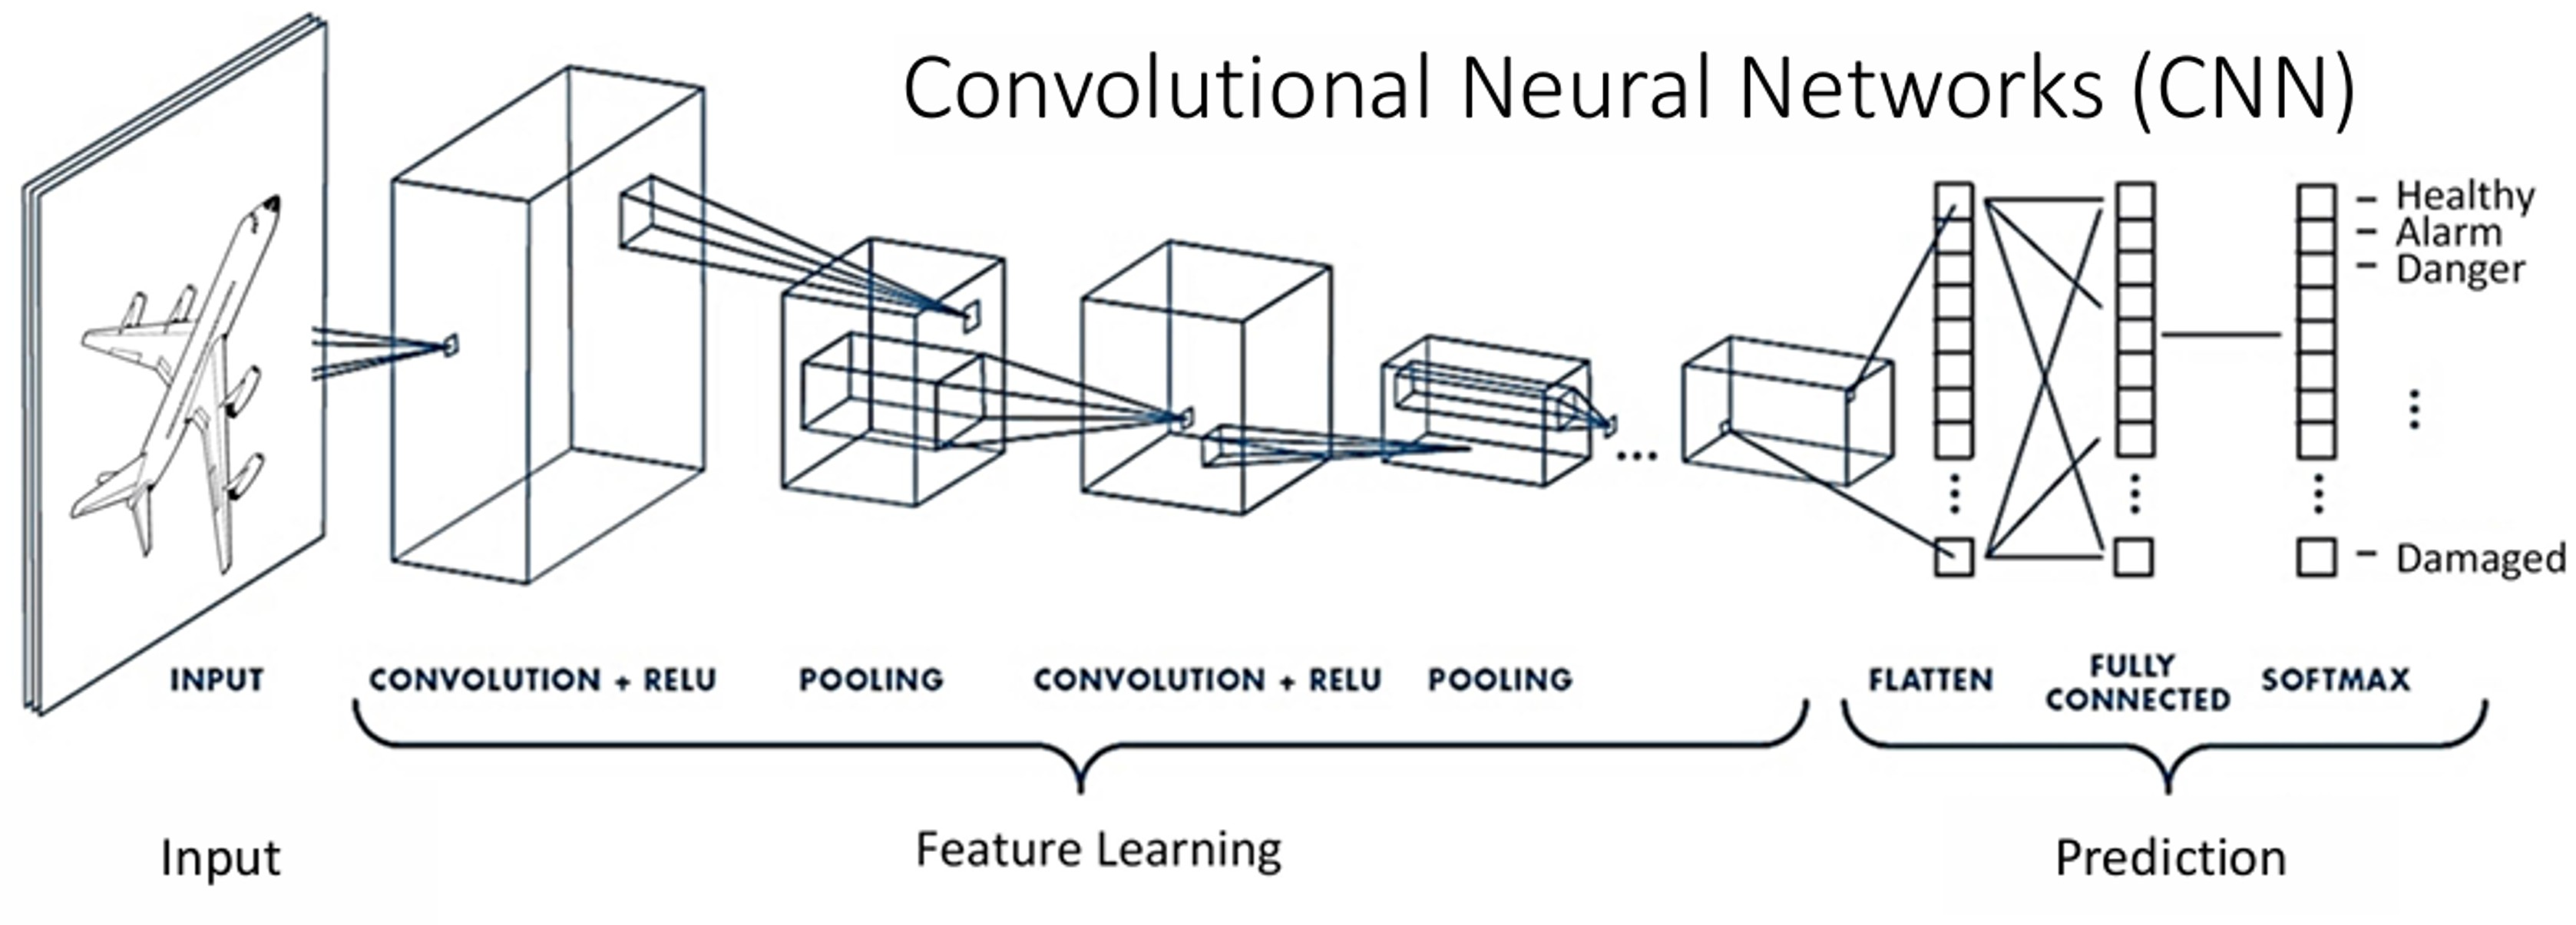
\includegraphics[width=0.8\linewidth]{CNN}}

\subsubsection{Popular CNN Architectures {\scriptsize \text{widely used CNN architectures include:}}}
\begin{itemize}[itemsep=0pt]
\item \textbf{VGG}: Deep networks with small $ 3 \times 3 $ filters.
\item \textbf{Inception}: Parallel convolution operations with different filter sizes.
\item \textbf{DenseNet}: Dense connections between layers.
\item \textbf{ResNet}: Residual connections to address vanishing gradients.
\end{itemize}

\textbf{CNN Applications}: \textit{Image Classification}: Identify objects in images (e.g. face emotion). \textit{Image Segmentation}: Detect regions of interest (e.g. cancer cell). \textbf{Object Detection}: Locate / classify objects (e.g. self-drive cars).

\columnbreak

\subsection{13. \underline{Recurrent Neural Networks (RNNs)}}
RNNs are a class of neural networks designed to process sequential data. 

\begin{itemize}
\item \textbf{Recurrent Neural Networks (RNNs)} maintain a \textbf{hidden state}, unlike traditional feedforward networks, which captures info of previous elements in sequence, enabling modelling temporal dependencies.
\item \textbf{Sequential data}, text -- context meaning of word), audio (phonemes interpretation) etc, has \textbf{patterns, dependencies} spanning across time steps. If elements treated independently, relationships btw. elements not captured. RNNs maintain \textbf{hidden state} ro encodes contextual information.
\item \textbf{One-hot Encoding}: method for converting categorical variables into a binary format (e.g. convert word to vector w. length equal to vocab size).
\item \textbf{Time step}:  single iteration in RNN, one element of sequence processed.
\item \textbf{Example}: `we saw this saw.', use one-hot encoding, represent word as vectors. Predict`saw' is verb or noun requires context of previous words. Standard feedforward network cannot capture this dependency, RNN can.
\end{itemize}

\subsubsection{Structure of an RNN}
An RNN processes sequential data, updating hidden state at each time step. 
\begin{itemize}
\item \textbf{Hidden State}: Number of elements in hidden state set according to no. of output we want to generate from each layer (e.g. 2 output $\leftrightarrow$ two elements)
\item Hidden state typically initialized to 0 ($h^0 = \mathbf{0}$).
\item Same \textbf{3 different weight matrices}, ($\mathbf{W}^{[xh]}, \mathbf{W}^{[hh]}, \mathbf{W}^{[hy]}$) applied at each time stamp. (weight for each edge)
\end{itemize}


The key equations governing an RNN are:
\begin{align*}
    \text{Updating }h: \quad \mathbf{h}^t &= g^{[h]}[(\mathbf{W}^{[xh]})^\top \mathbf{x}^t + (\mathbf{W}^{[hh]})^\top \mathbf{h}^{t-1}] \\
    \text{Predicting Output:} \quad \hat{\mathbf{y}}^t &= g^{[y]}[(\mathbf{W}^{[hy]})^\top \mathbf{h}^t]
\end{align*}
\begin{itemize}[itemsep=0pt]
\item $\mathbf{x}^t$: Input at time step $t$, \quad $\mathbf{h}^t$: Hidden state at time step $t$
\item $\hat{\mathbf{y}}^t$: Output prediction at $t$ \quad $\mathbf{g}^{[h]}$, $\mathbf{g}^{[y]}$: Activation Fn (sigmoid, softmax).
\end{itemize}
\centerline{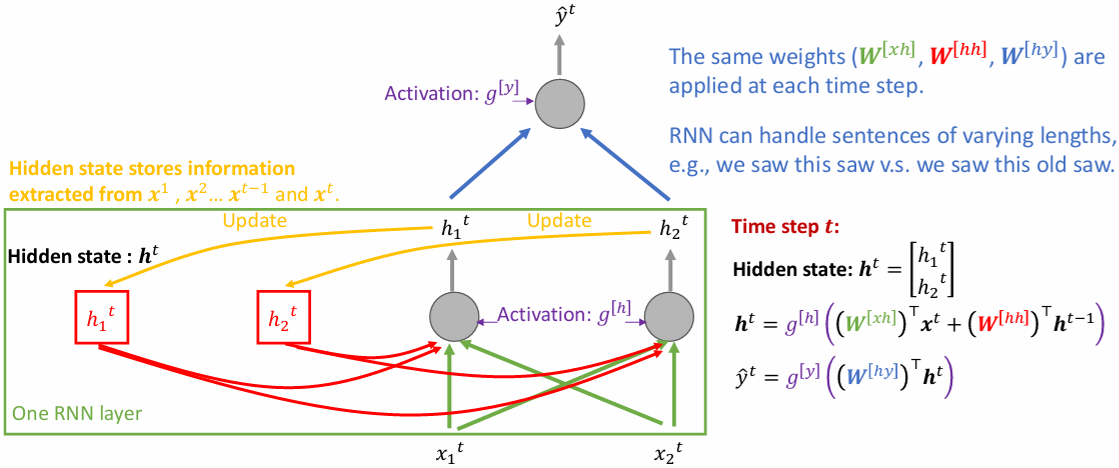
\includegraphics[width=0.95\linewidth]{RNN}}
\hrule
\centerline{\includegraphics[width=0.9\linewidth]{RNNCalc}}

The hidden state $\mathbf{h}^t$ acts as a memory that stores information about past inputs. At each time step, the RNN combines the current input $\mathbf{x}^t$ with the previous hidden state $\mathbf{h}^{t-1}$ to compute the new hidden state.

\subsubsection{Types of RNN Architectures {\scriptsize (Configuration depending on task) }}
\begin{itemize}
    \item \textbf{Many-to-Many ($T_x = T_y > 1$)}: Both input and output sequences have the same length. E.g.: Machine translation (e.g., Eng to French).
    \item \textbf{Many-to-One ($T_x > 1, T_y = 1$)}: A sequence of inputs produces a single output. E.g.: Sentiment analysis (review positive or neg).
\end{itemize}
\centerline{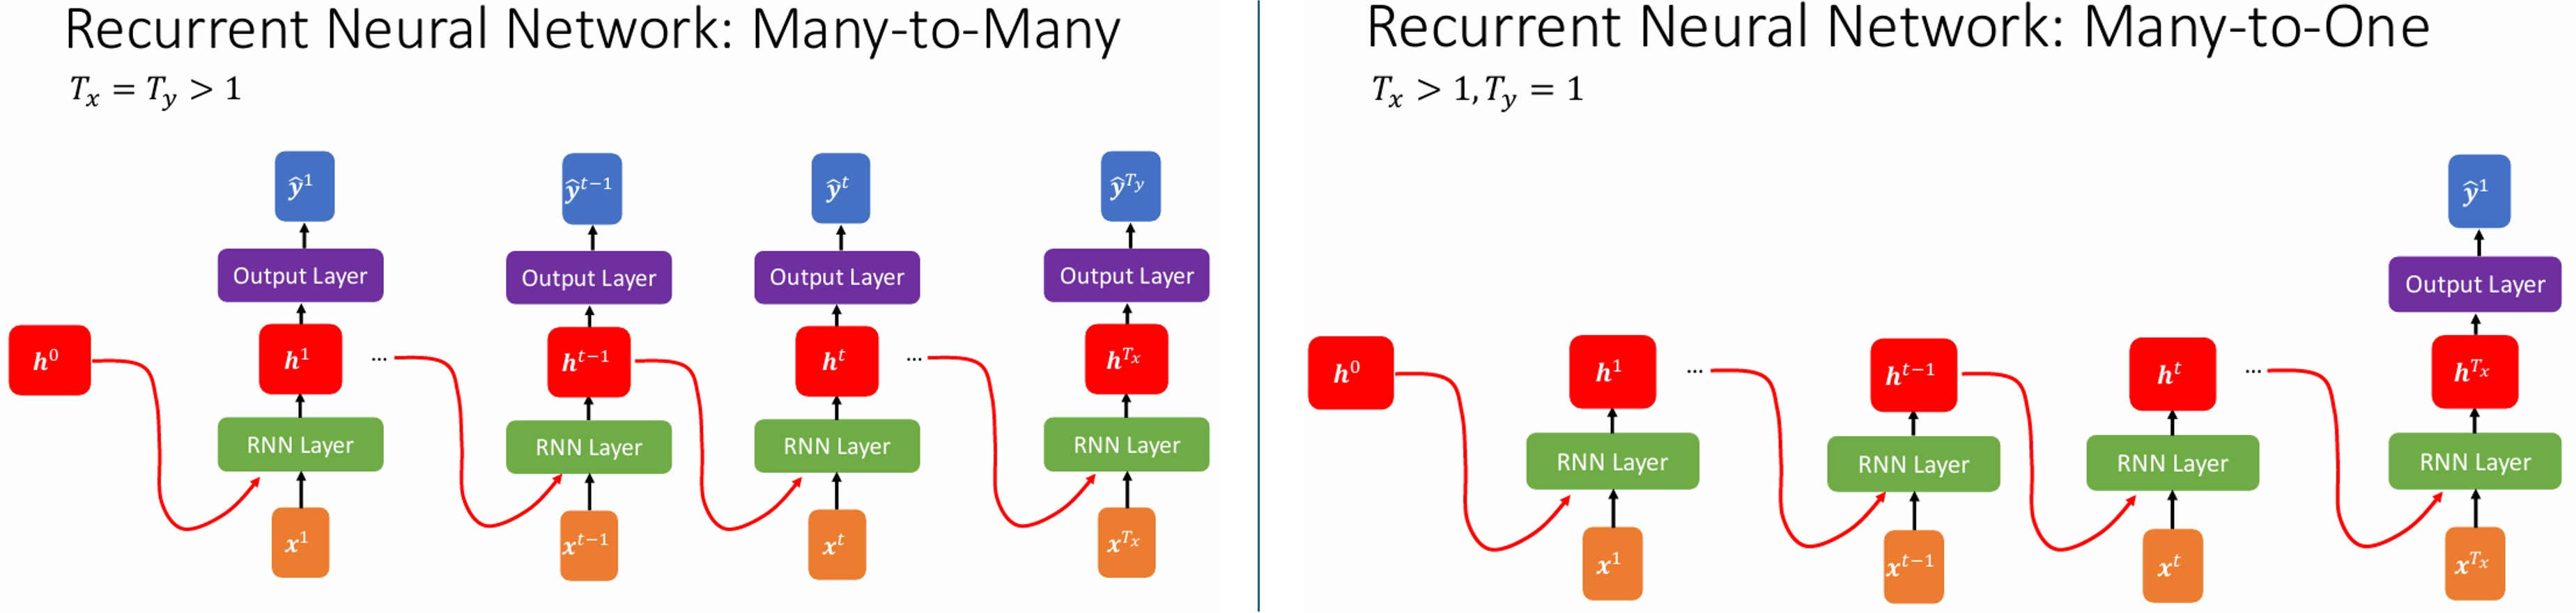
\includegraphics[width=1\linewidth]{many-to-many-1}}
\begin{itemize}
    \item \textbf{One-to-Many ($T_x = 1, T_y > 1$)}: A single input generates sequence of outputs. E.g.: Image captioning (e.g. generate image description).
    \item \textbf{Many-to-Many ($T_x \neq T_y, T_x > 1, T_y > 1$)}: Input and output sequences have different lengths. Has $<$begin$>$ token. E.g.: Video captioning.
\end{itemize}
\centerline{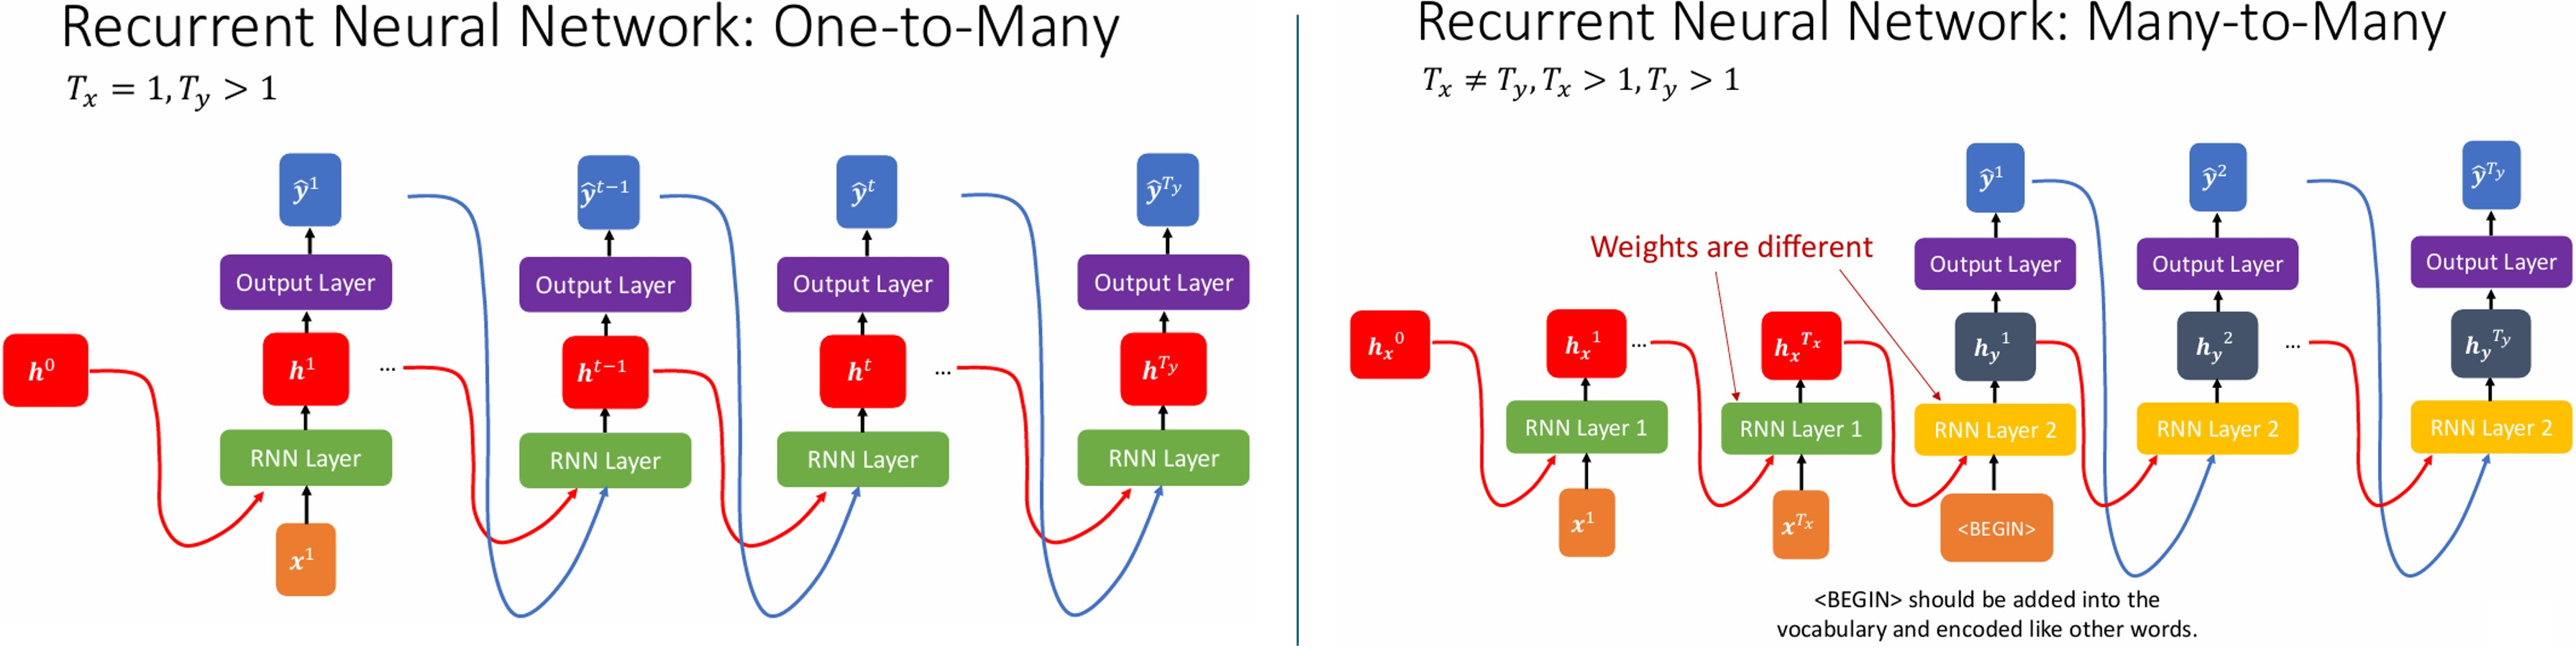
\includegraphics[width=1\linewidth]{many-to-many-2}}
\subsubsection{Deep Recurrent Neural Networks}
Deep RNNs capture more complex hierarchical features by stacking multiple recurrent layers. Each layer processes hidden state from previous layer, allow network to learn more abstract representations of input sequence.
\centerline{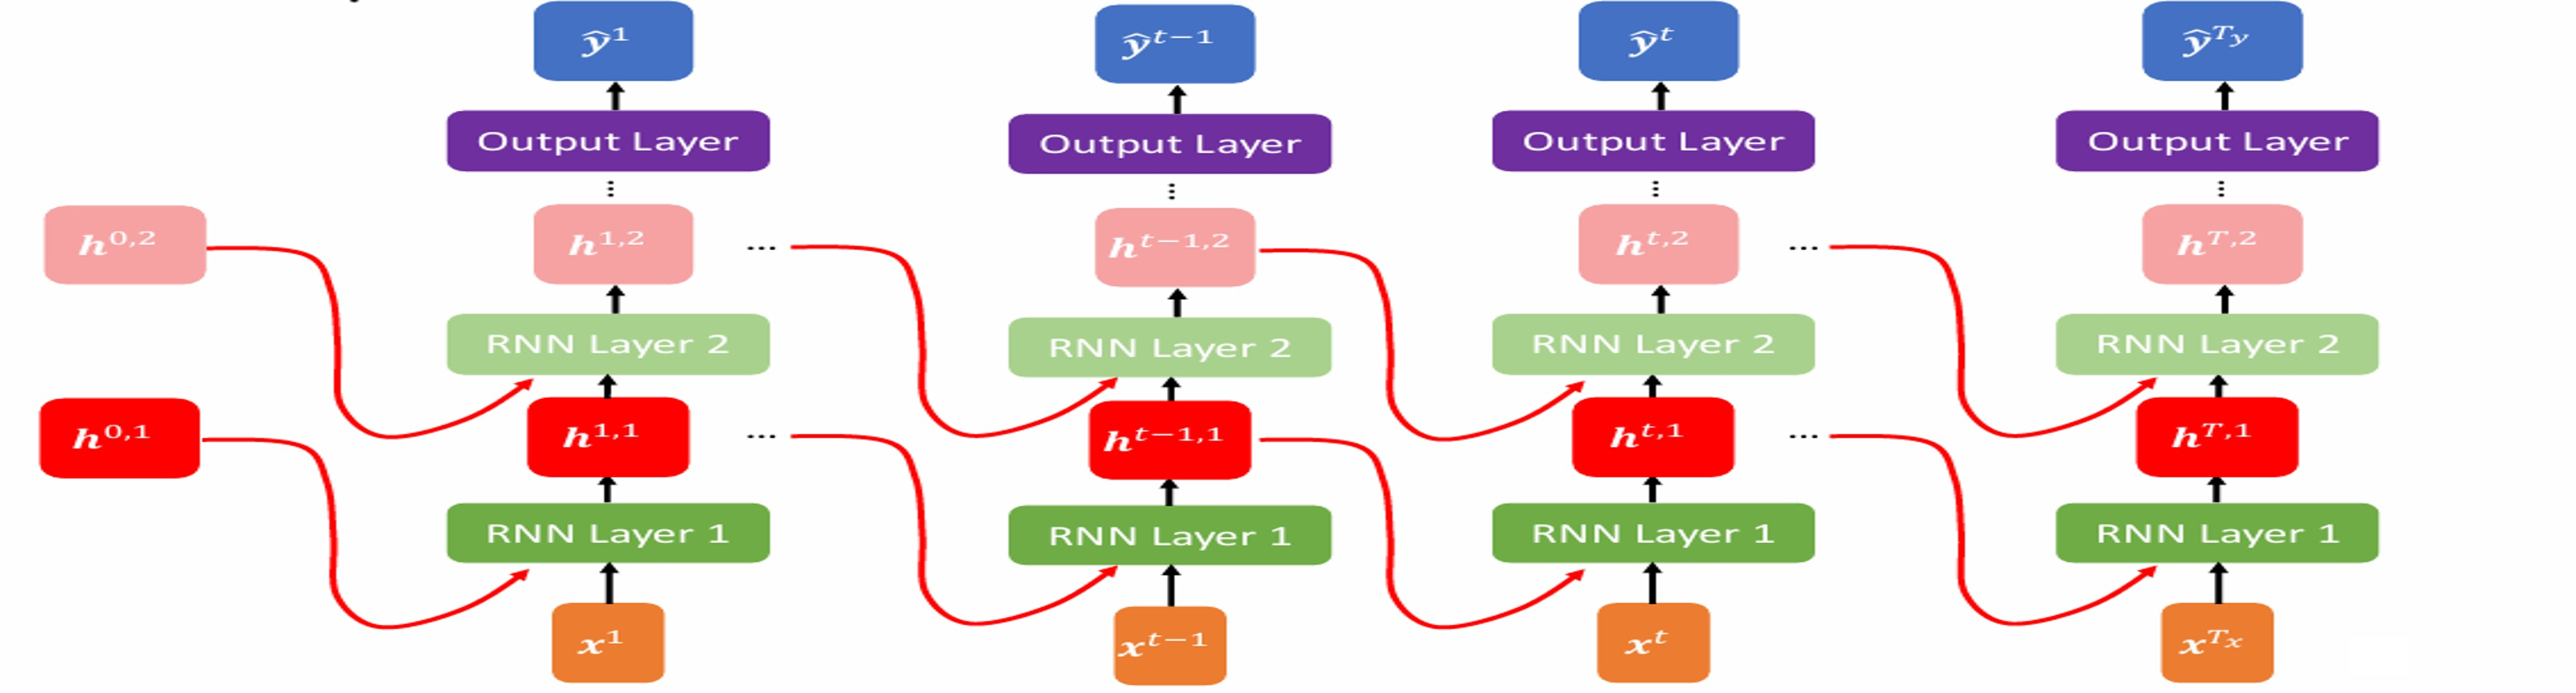
\includegraphics[width=1\linewidth]{deepRNN}}

\begin{itemize}
	\item \textbf{Application of RNNs}: widely used in tasks involving sequential data, such as \textit{Sentiment Analysis}, \textit{Speech Recognition}: Transcribing spoken language into text, \textit{Video Captioning}: Generating descriptions for video frames.
	\item \textbf{Properties of RNN}: \textit{Capture Contextual Information}: RNNs use hidden state to encode information about entire sequence seen so far. \textbf{Sequential in Nature}: Predictions at time step $t$ depend on all previous steps, less parallelism-friendly than feedforward networks.
\end{itemize}

% -----------------------------------------------------------------------------------------

\subsection{14. \underline{Attention Neural Networks: Self-Attention (Layer)}}
Mechanism that captures contextual information, identify relevant parts of input sequence. Allows model to aggregate useful info from all elements in sequence, to predict current output. $\rightarrow$ can handle sequential data.

\begin{itemize}
\item \textbf{Query ($Q$)}: Represents current element being processed.
\item \textbf{Key ($K$)}: Encodes relevance of other elements in sequence to the query.
\item \textbf{Value ($V$)}: Contains the actual content or information to be aggregated.
\end{itemize}
Components derived from input sequence using trainable weight matrices:
$$
Q = W^qX, \quad K = W^kX, \quad V = W^vX,
$$
where $X$ is (\textbf{column major input matrix}, each column correspond to single feature vector e.g. 
$\begin{bmatrix}
x_1 & y_1 & z_2\\
x_2 & y_2  & z_2\\
\end{bmatrix}$), and $W^q$, $W^k$, $W^v$ are the weight matrices for queries, keys, and values, respectively. \\

\centerline{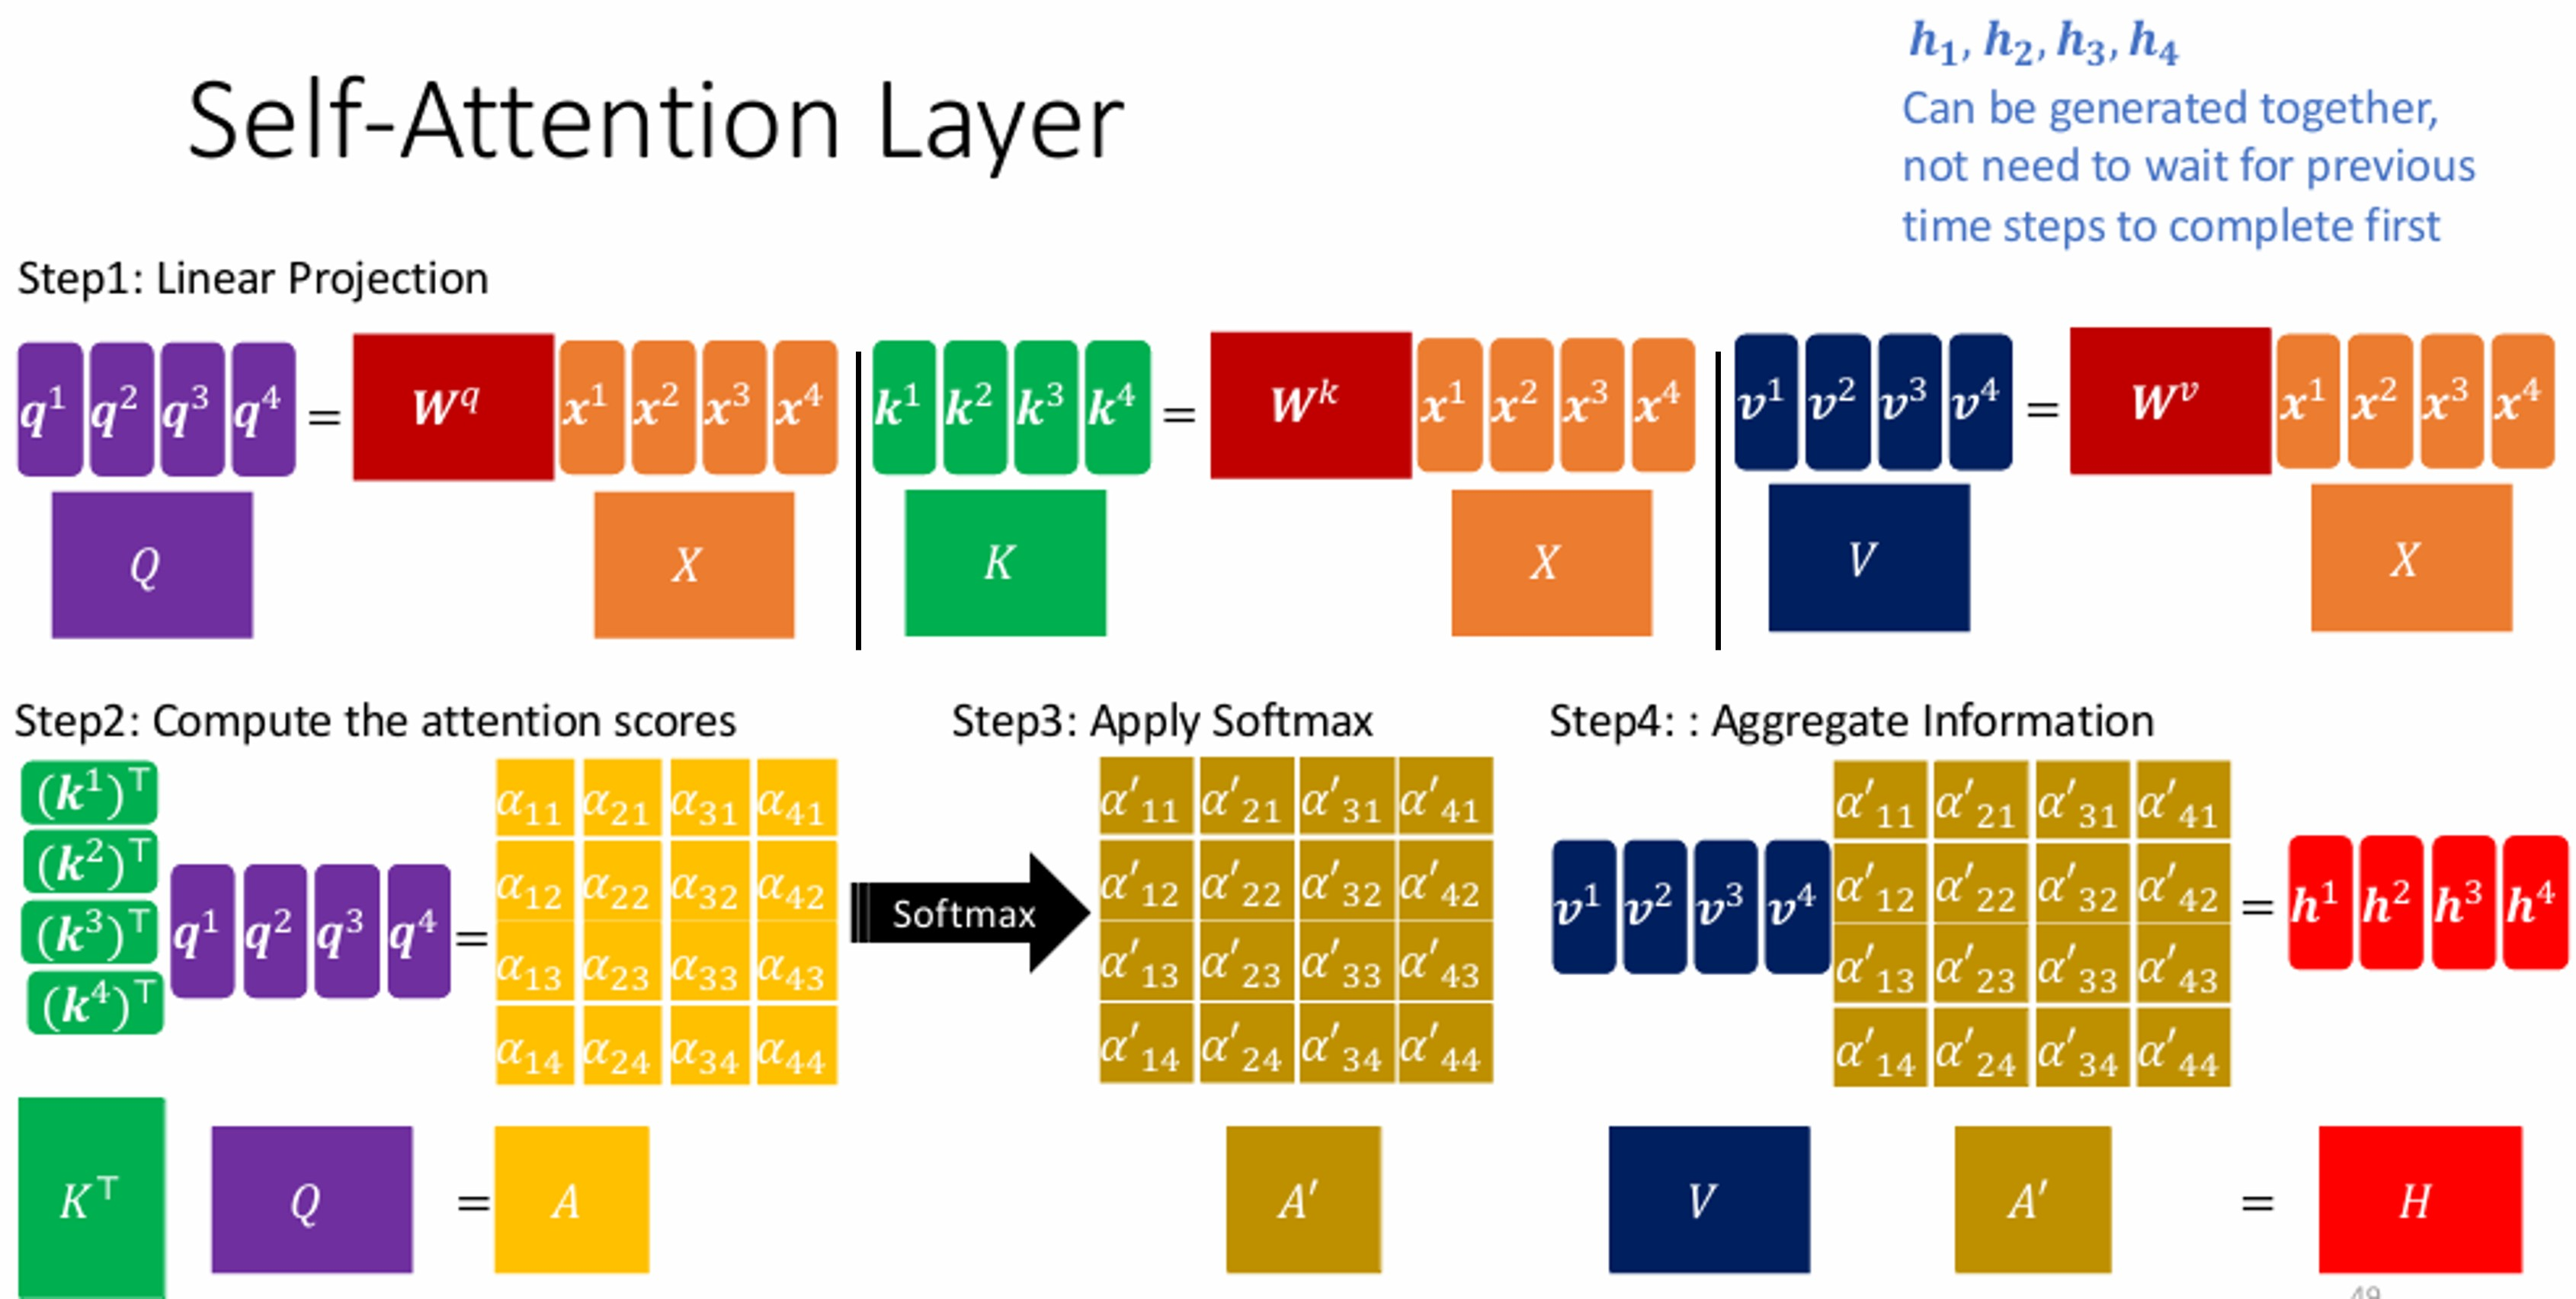
\includegraphics[width=1\linewidth]{matrixRNN}}

\subsubsection{Steps in Self-Attention Mechanism}
\begin{enumerate}
\item \textbf{Linear Projection}: Each input vector $x_i$ is transformed into query, key, and value vectors:
$q_i = W_Q x_i, \quad k_i = W_K x_i, \quad v_i = W_V x_i$
\item \textbf{Compute Attention Scores}: attention scores measure relevance of each element in sequence to current query: 
$\alpha_{ij} = k_j^\top q_i$ \\
$k_j$: key vector for $j$-th element, $q_i$: query vector for $i$-th element.
\item \textbf{Apply Softmax}: attention scores are normalized using softmax function to obtain probabilities:
$\alpha'_{ij} = \frac{\exp(\alpha_{ij})}{\sum_{j} \exp(\alpha_{ij})}$
\item \textbf{Aggregate Information}: Final output for $i$-th element is a weighted sum of value vectors:
$h_i = \sum_{j} \alpha'_{ij} v_j$\\
$\alpha'_{ij}$': normalized attention score, $v_j$: value vector for $j$-th element.
\end{enumerate}
%% Example
\centerline{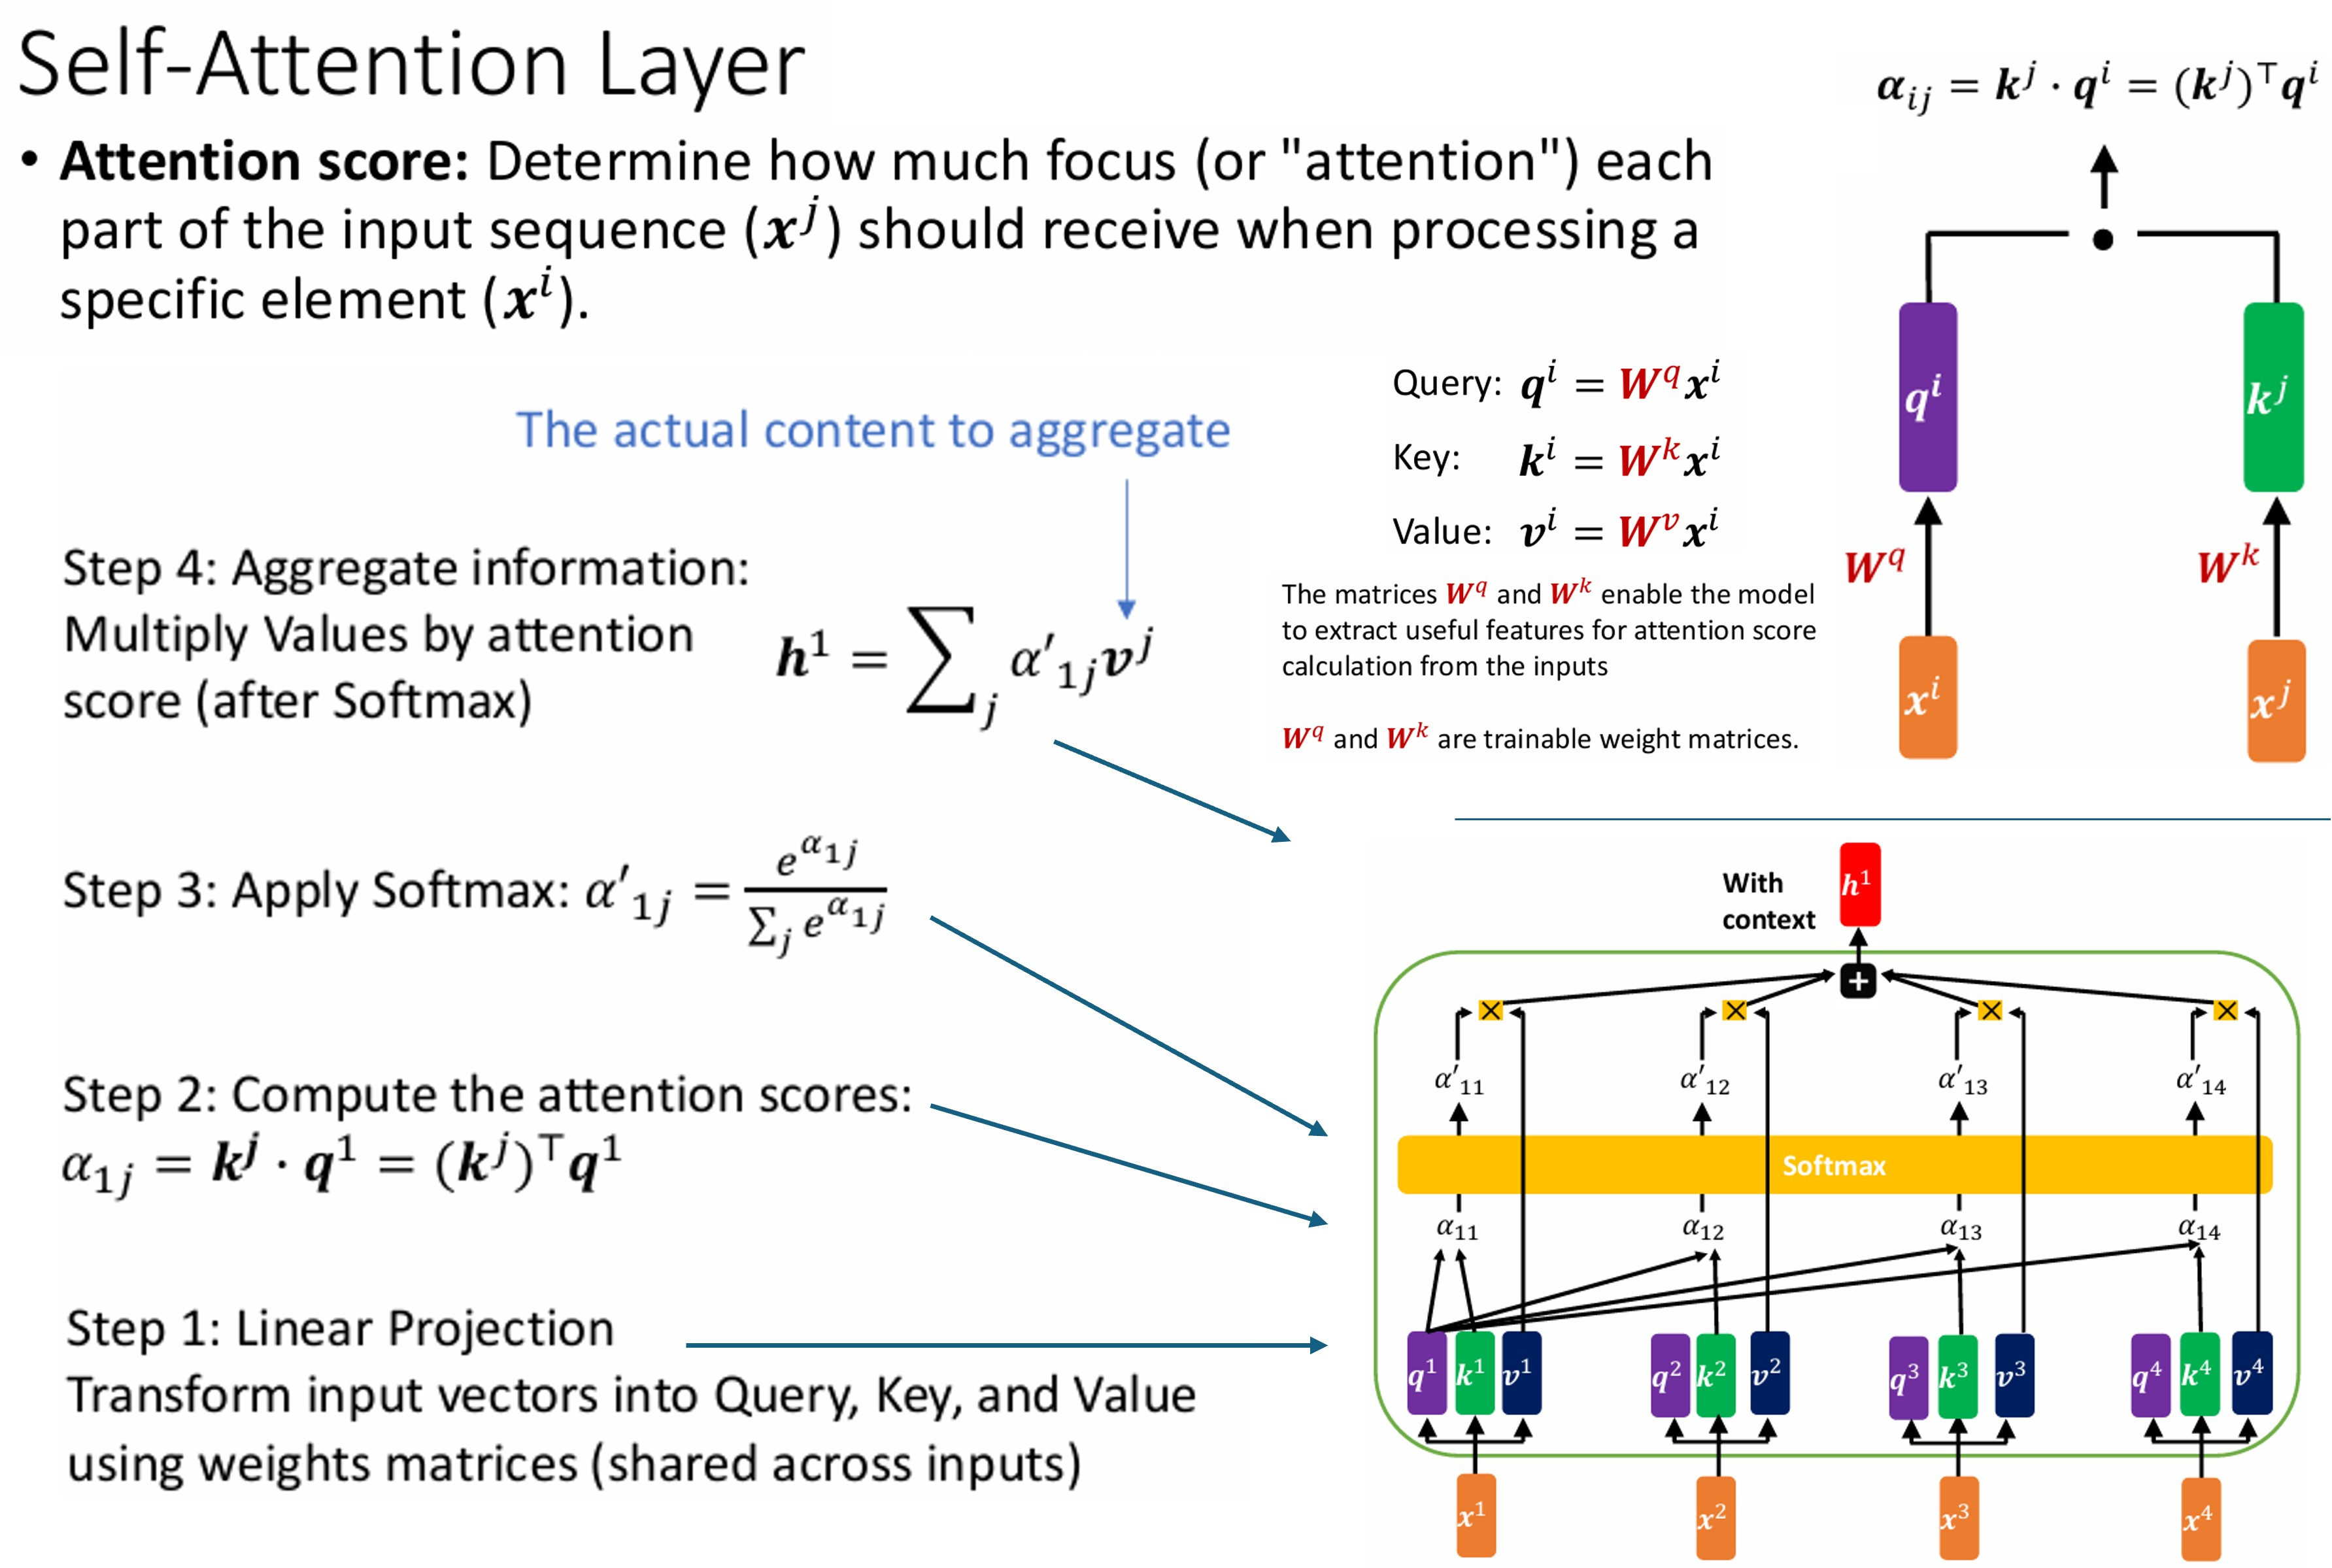
\includegraphics[width=1\linewidth]{selfAttentionLayer}}

\begin{itemize}
\item \textbf{Advantages of Self-Attention}: Captures long-range dependencies in input sequence, does not require sequential processing, can parallel compute, 
context-aware representations for each element in sequence.
\item \textbf{Applications}: Self-attention core component of transformer architectures, widely used in NLP, (machine translation, text summarization), Computer Vision (Vision Transformers (ViTs), image classification), Speech Processing (speech recognition, synthesis).
\item \textbf{Still requires Positional Encoding}: "we saw this saw.": One-hot encoding to represent words, input vectors to self-attention layer, generate outputs. But, \textbf{positional encoding} still needed to generate diff outputs for diff `saw' instances.
\end{itemize}

\subsubsection{Positional Encoding}
Technique to inject positional information into input features, e.g. one-hot vectors, to enable models like Transformers to capture order of elements.
\begin{itemize}
\item \textbf{Purpose}: Explicitly encode the position of each token in the sequence.
\item \textbf{Formula}: The positional encoding vector $ PE_i $ for position $ i $ is added to the original input feature vector $ x_i $: 
\quad $[x'_i = x_i + PE_i]$.\\
- $ x_i \in \mathbb{R}^d $: Original input feature vector for position $ i $,\\
- $ PE_i \in \mathbb{R}^d $: Positional encoding vector for position $ i $,\\
- $ x'_i \in \mathbb{R}^d $: Final input feature vector after adding positional encoding.
\item \textbf{Generating Positional Encoding Using Sine and Cosine Functions}:

The positional encoding values are computed using sine and cosine functions:
$$
PE_{i, 2k} = \sin\left(\frac{i}{10000^{\frac{2k}{d}}}\right), \quad PE_{i, 2k+1} = \cos\left(\frac{i}{10000^{\frac{2k}{d}}}\right)
$$  
- $ i $: Position index (starting from 0), \quad $ d $: Input feature dimension.\\
- $ k $: Dimension index (starting from 0, goes up to $\frac{d}{2} - 1$) \\    
- In this case, Dimension tells whether to use sine or cosine.
\item \textbf{Example}: Generate Positional Encoding for input feature dimension $ d = 4 $
    $$
    \text{For $ i = 1 $}: PE_1 =
    \begin{bmatrix}
    \sin(1) \text{\tiny (k=0)}\\
    \cos(1) \text{\tiny (k=0)}\\
    \sin\left(\frac{1}{100}\right) \text{\tiny (k=1)} \\
    \cos\left(\frac{1}{100}\right) \text{\tiny (k=1)}
    \end{bmatrix}.
 	\text{For $ i = 2 $}: PE_2 =
    \begin{bmatrix}
    \sin(2) \\
    \cos(2) \\
    \sin\left(\frac{1}{50}\right) \\
    \cos\left(\frac{1}{50}\right)
    \end{bmatrix}.
    $$
    
\item \textbf{Why Positional Encoding is Necessary}: Enable self-attention layers to distinguish btw. identical tokens at different positions. (e.g. Both instances of "saw" would have same representation if only one-hot encoding is used.)
\item Positional encoding ensures that sequential models can capture the order of elements in the input sequence. It is particularly important in architectures like Transformers, which do not inherently process sequences in order.
\end{itemize}

\subsection{Issues with Deep Learning}
\subsubsection{Overfitting}
Occurs when model learns to fit training data too closely, capturing noise and irrelevant patterns instead of generalizing well to unseen data.
\begin{itemize}
\item \textbf{Causes of Overfitting}: Model overly complex (e.g., too many params), insufficient training data, training too many epochs w/o proper regularization.
\item \textbf{Solutions to Overfitting}:
	\begin{itemize}
	\item \textbf{Dropout}: During training, randomly set some neurons' outputs to zero with a given probability. Prevents model from relying too heavily on specific neurons, encouraging robustness.
	\item \textbf{Early Stopping}: Monitor the validation loss during training. Stop training when validation loss stops improving, even if training loss continues to decrease. Prevents the model from over-optimizing on the training data.
	\item \textbf{Regularization}: Add penalty terms (e.g., L1 or L2 regularization) to loss function to discourage large weights.
	\item \textbf{Data Augmentation}: Increase size, diversity of training dataset by applying transformations (e.g., rotations, flips, noise).
	\end{itemize}
\end{itemize}

\subsubsection{Vanishing and Exploding Gradients}
Training deep neural networks involves backpropagation, where gradients are computed and propagated backward through the layers. Issues:
\begin{enumerate}
\item \textbf{Vanishing Gradient}: Small gradients get multiplied repeatedly as they propagate backward through layers, eventually becoming almost zero.
Prevents earlier layers from learning effectively.
	\begin{itemize}
	\item \textbf{Mitigation Strategies for Vanishing Gradients}: Use activation functions that avoid saturation (e.g., ReLU instead of sigmoid or tanh), Normalize inputs and use techniques like Batch Normalization to stabilize gradients, Employ residual connections in architectures like ResNet to allow gradients to flow directly.
	\end{itemize}
\item \textbf{Exploding Gradient}: Large gradients get multiplied repeatedly, causing numerical instability or overflow. Destabilizes training process.
	\begin{itemize}
	\item \textbf{Mitigation Strategies for Exploding Gradients}: Apply gradient clipping: Clip gradients to a specified range (e.g., $[-\text{clip\_value}, \text{clip\_value}]$). Use weight initialization techniques (e.g., Xavier or He initialization) to prevent large initial gradients.
	\end{itemize}
\end{enumerate}

\subsection{\underline{Attention Neural Networks}}

Attention mechanisms in modern neural network architectures, enable model to focus on relevant parts of input sequence when making predictions. Different types of attention neural networks and applications:

\begin{itemize}
\item \textbf{Many-to-Many Attention}: where input and output sequences same length.
\end{itemize}
\centerline{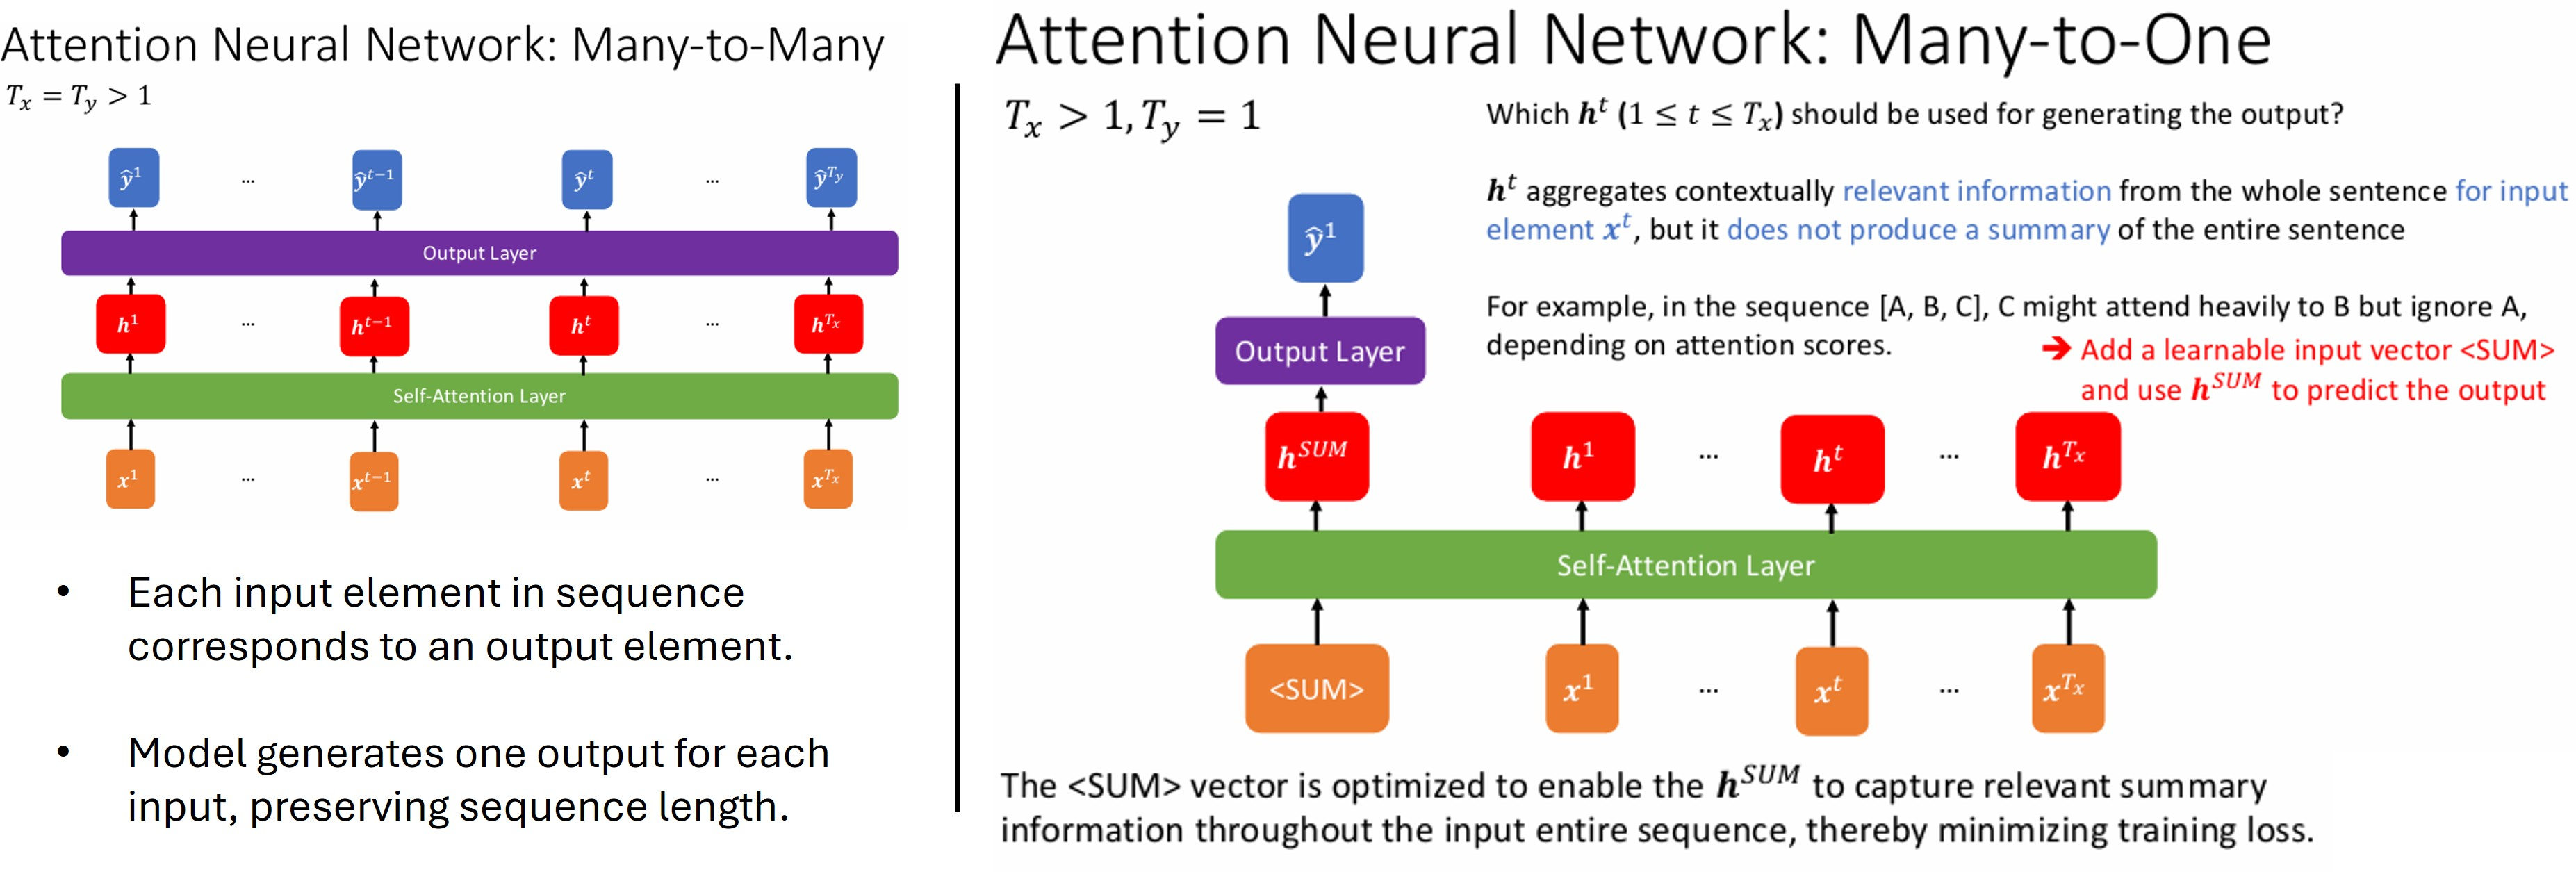
\includegraphics[width=1\linewidth]{attentionNN1}}

\begin{itemize}
\item \textbf{Many-to-One Attention}: In such networks, input sequence processed to produce a single output. (tasks e.g. sentiment analysis, classification).
	\begin{itemize}
	\item Each hidden state $ h_t $ aggregates contextually relevant info from entire input sequence. But, each $ h_t $ does not summarize the entire sequence.
	\item $h^t$ position-specific focused, summary $h^{\texttt{SUM}}$ captures global context.
	\item \textbf{Aggregation of Contextual Information}: To address this, special learnable token (e.g., \texttt{<SUM>} learnable input vector) added  to capture a summary representation, and use $h^{\texttt{SUM}}$ to predict output:
	  $$
	  \text{e.g.}: \quad h_{\text{SUM}} = \sum_j \alpha'_j v_j, \quad \text{$ \alpha'_j $ are normalized attention weights.}
	  $$
	\end{itemize}
\item \textbf{One-to-Many Attention}: A single input ($ x_1 $) generates sequence of multiple outputs, where $ T_x = 1 $ and $ T_y > 1 $ (e.g. text generation).
	\begin{itemize}
	\item First generates first output $ \hat{y}_1 $ via hidden state $ h_1 $. Subsequent outputs $ \hat{y}_2, \hat{y}_3, \dots $ generated sequentially, incorporate previously predicted tokens $ \hat{y}_1, \hat{y}_2, \dots $ as context.
	\item \textbf{Masked Self-Attention}: To ensure model only uses previously generated tokens during prediction, masked self-attention is applied.
  $$
  \text{Masked Attention Scores} = 
  \begin{bmatrix}
  0 & -\infty & -\infty \\
  0 & 0 & -\infty \\
  0 & 0 & 0
  \end{bmatrix}, \text{for softmax function}
  $$
Diagonal, lower triangular entries set to $ 0 $ (allow attention to current, past tokens). Upper triangular set to $ -\infty $ (blocking attention to future tokens).
\item \texttt{ADD} mask after compute attention scores, prevent attending to future tokens (cheating). Maintains causal prediction, as during training, in techniques like teacher forcing, ground truth tokens ($ y_1, y_2, \dots $) provided. 
\item Without mask, model could "cheat" by attending to future tokens, leading to overfitting and poor generalization during inference.
	\end{itemize}
\end{itemize}
\centerline{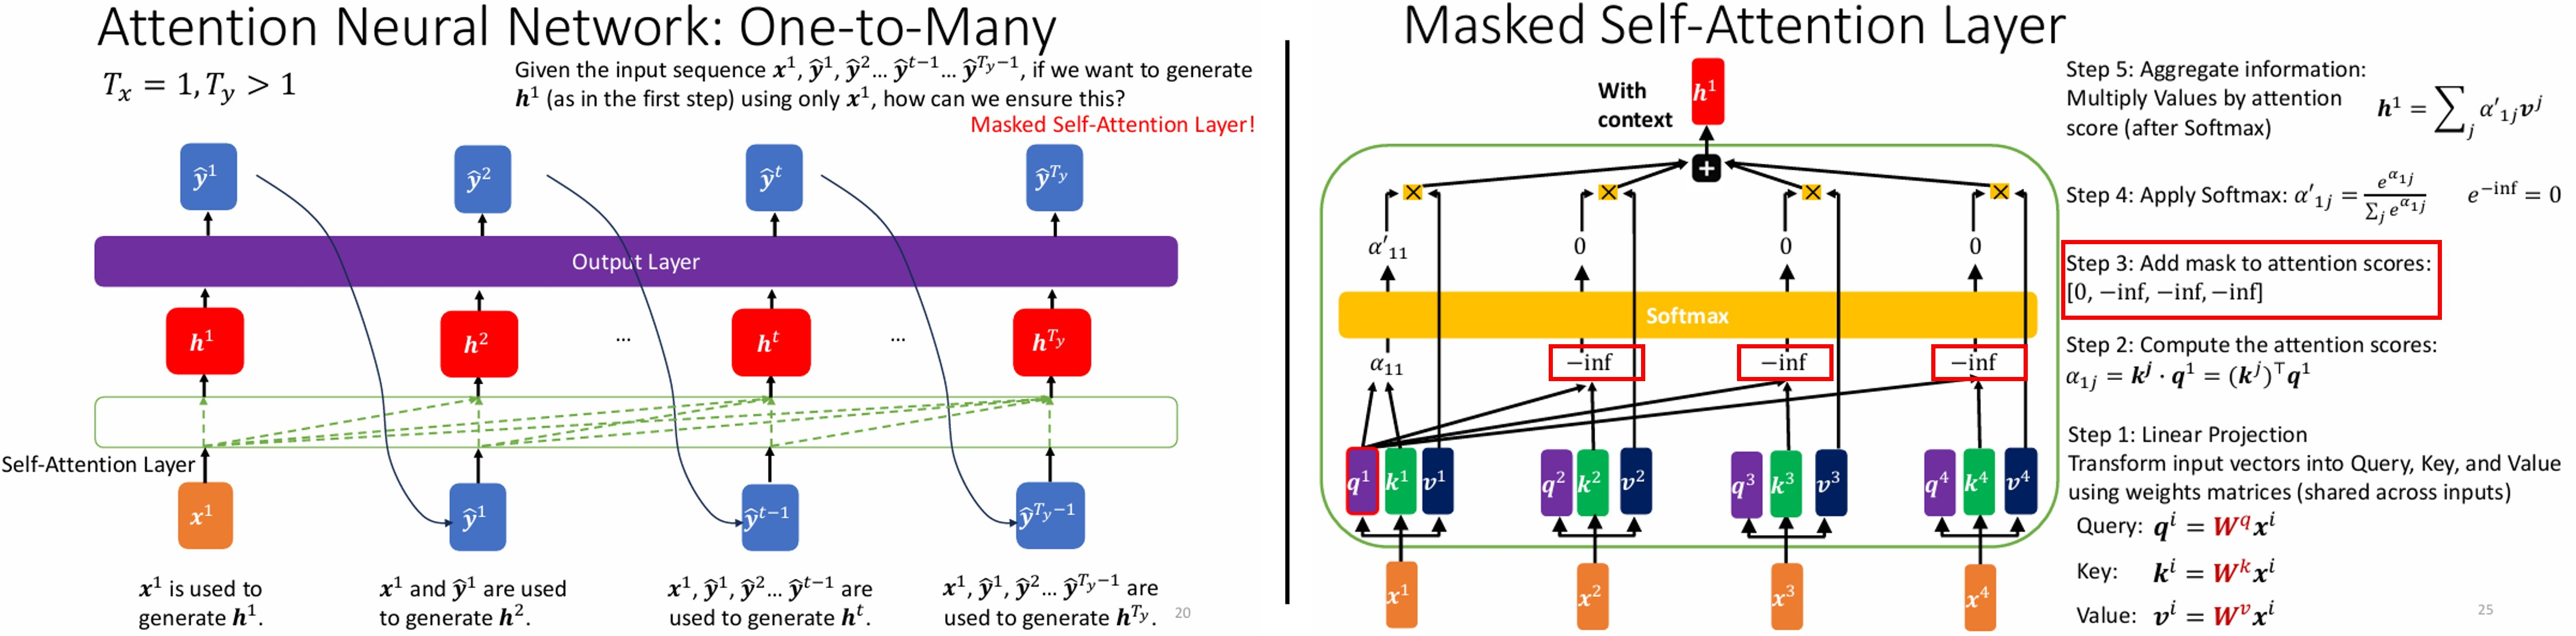
\includegraphics[width=1\linewidth]{attentionNN2}}
 
 % --------- 
  
\subsubsection{Many-to-Many Attention {\scriptsize (input/output sequence different lengths)}}
\centerline{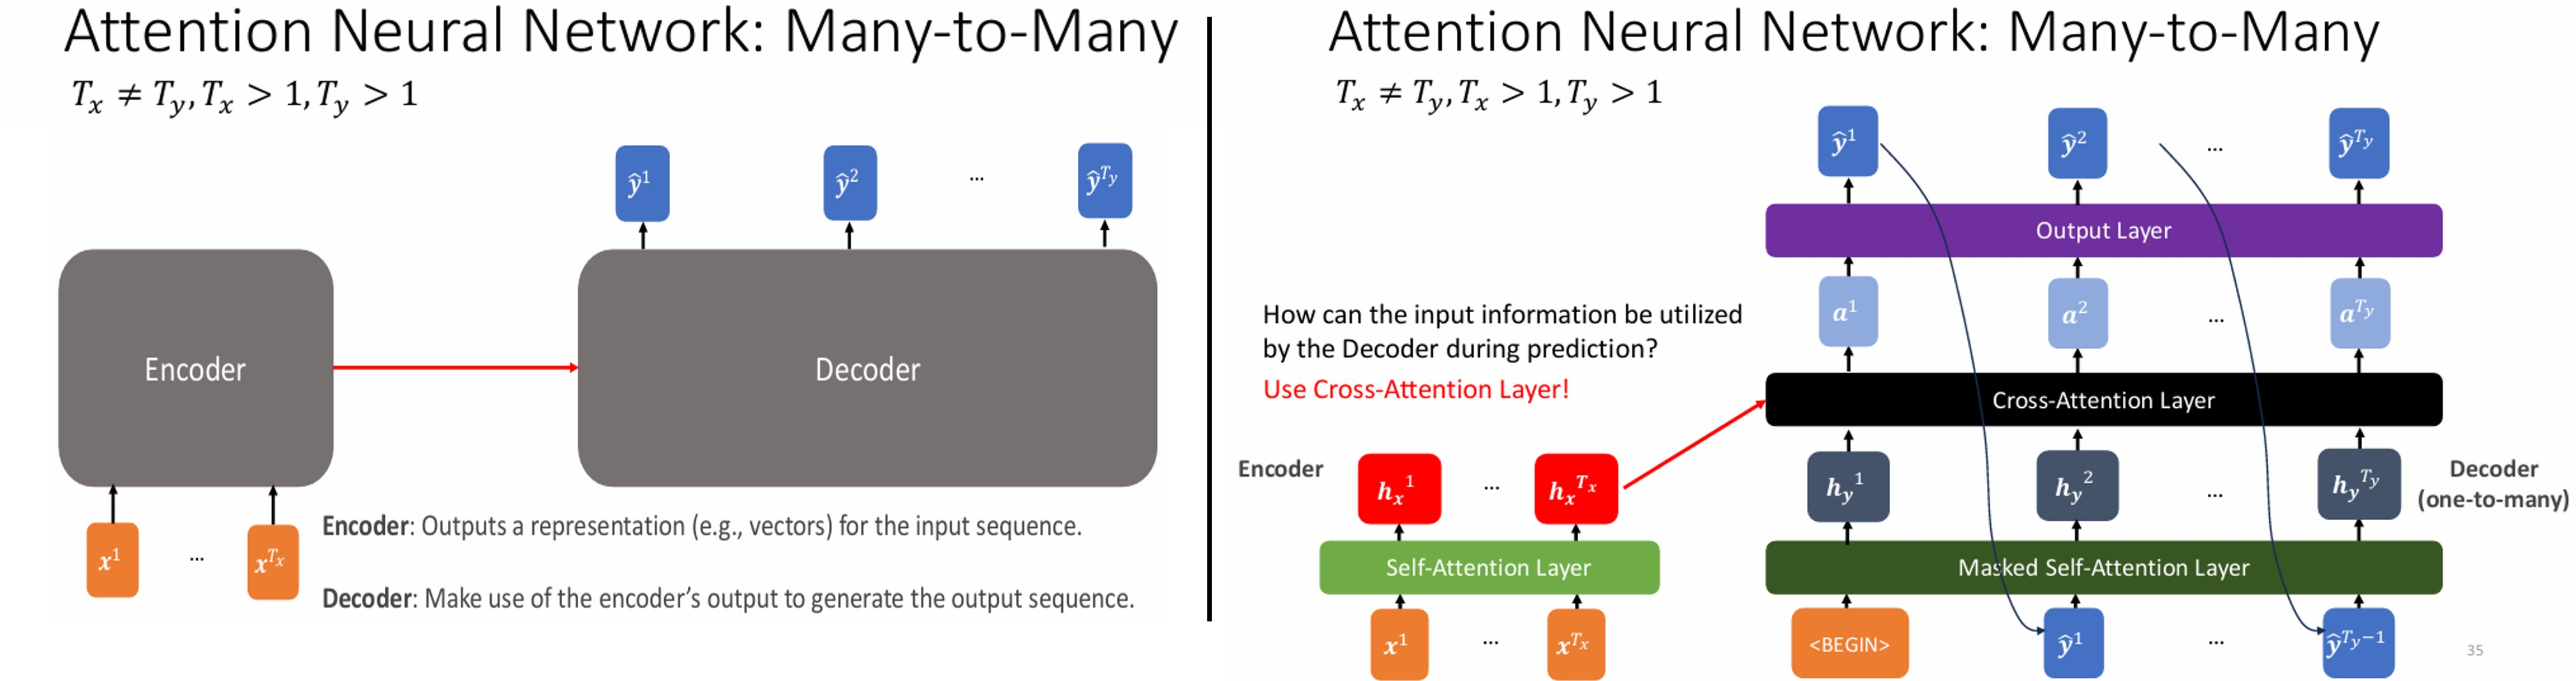
\includegraphics[width=1\linewidth]{attentionNN3}}
\begin{itemize}
\item \textbf{Encoder-Decoder Architecture}: Encoder process input sequence, produce contextual representation. Decoder uses repn. to generate output sequence.
\item \textbf{Cross-Attention Layer}: enables decoder to focus on relevant parts of the encoder's output while generating each token in the output sequence. Operates by computing attention scores between:
	\begin{itemize}
	\item \textbf{Query}: ($Q$): Derived from \underline{decoder's} hidden states.
	\item \textbf{Key ($K$) and Value ($V$)}: Derived from the \underline{encoder's} output.
	\end{itemize}
\end{itemize}
\centerline{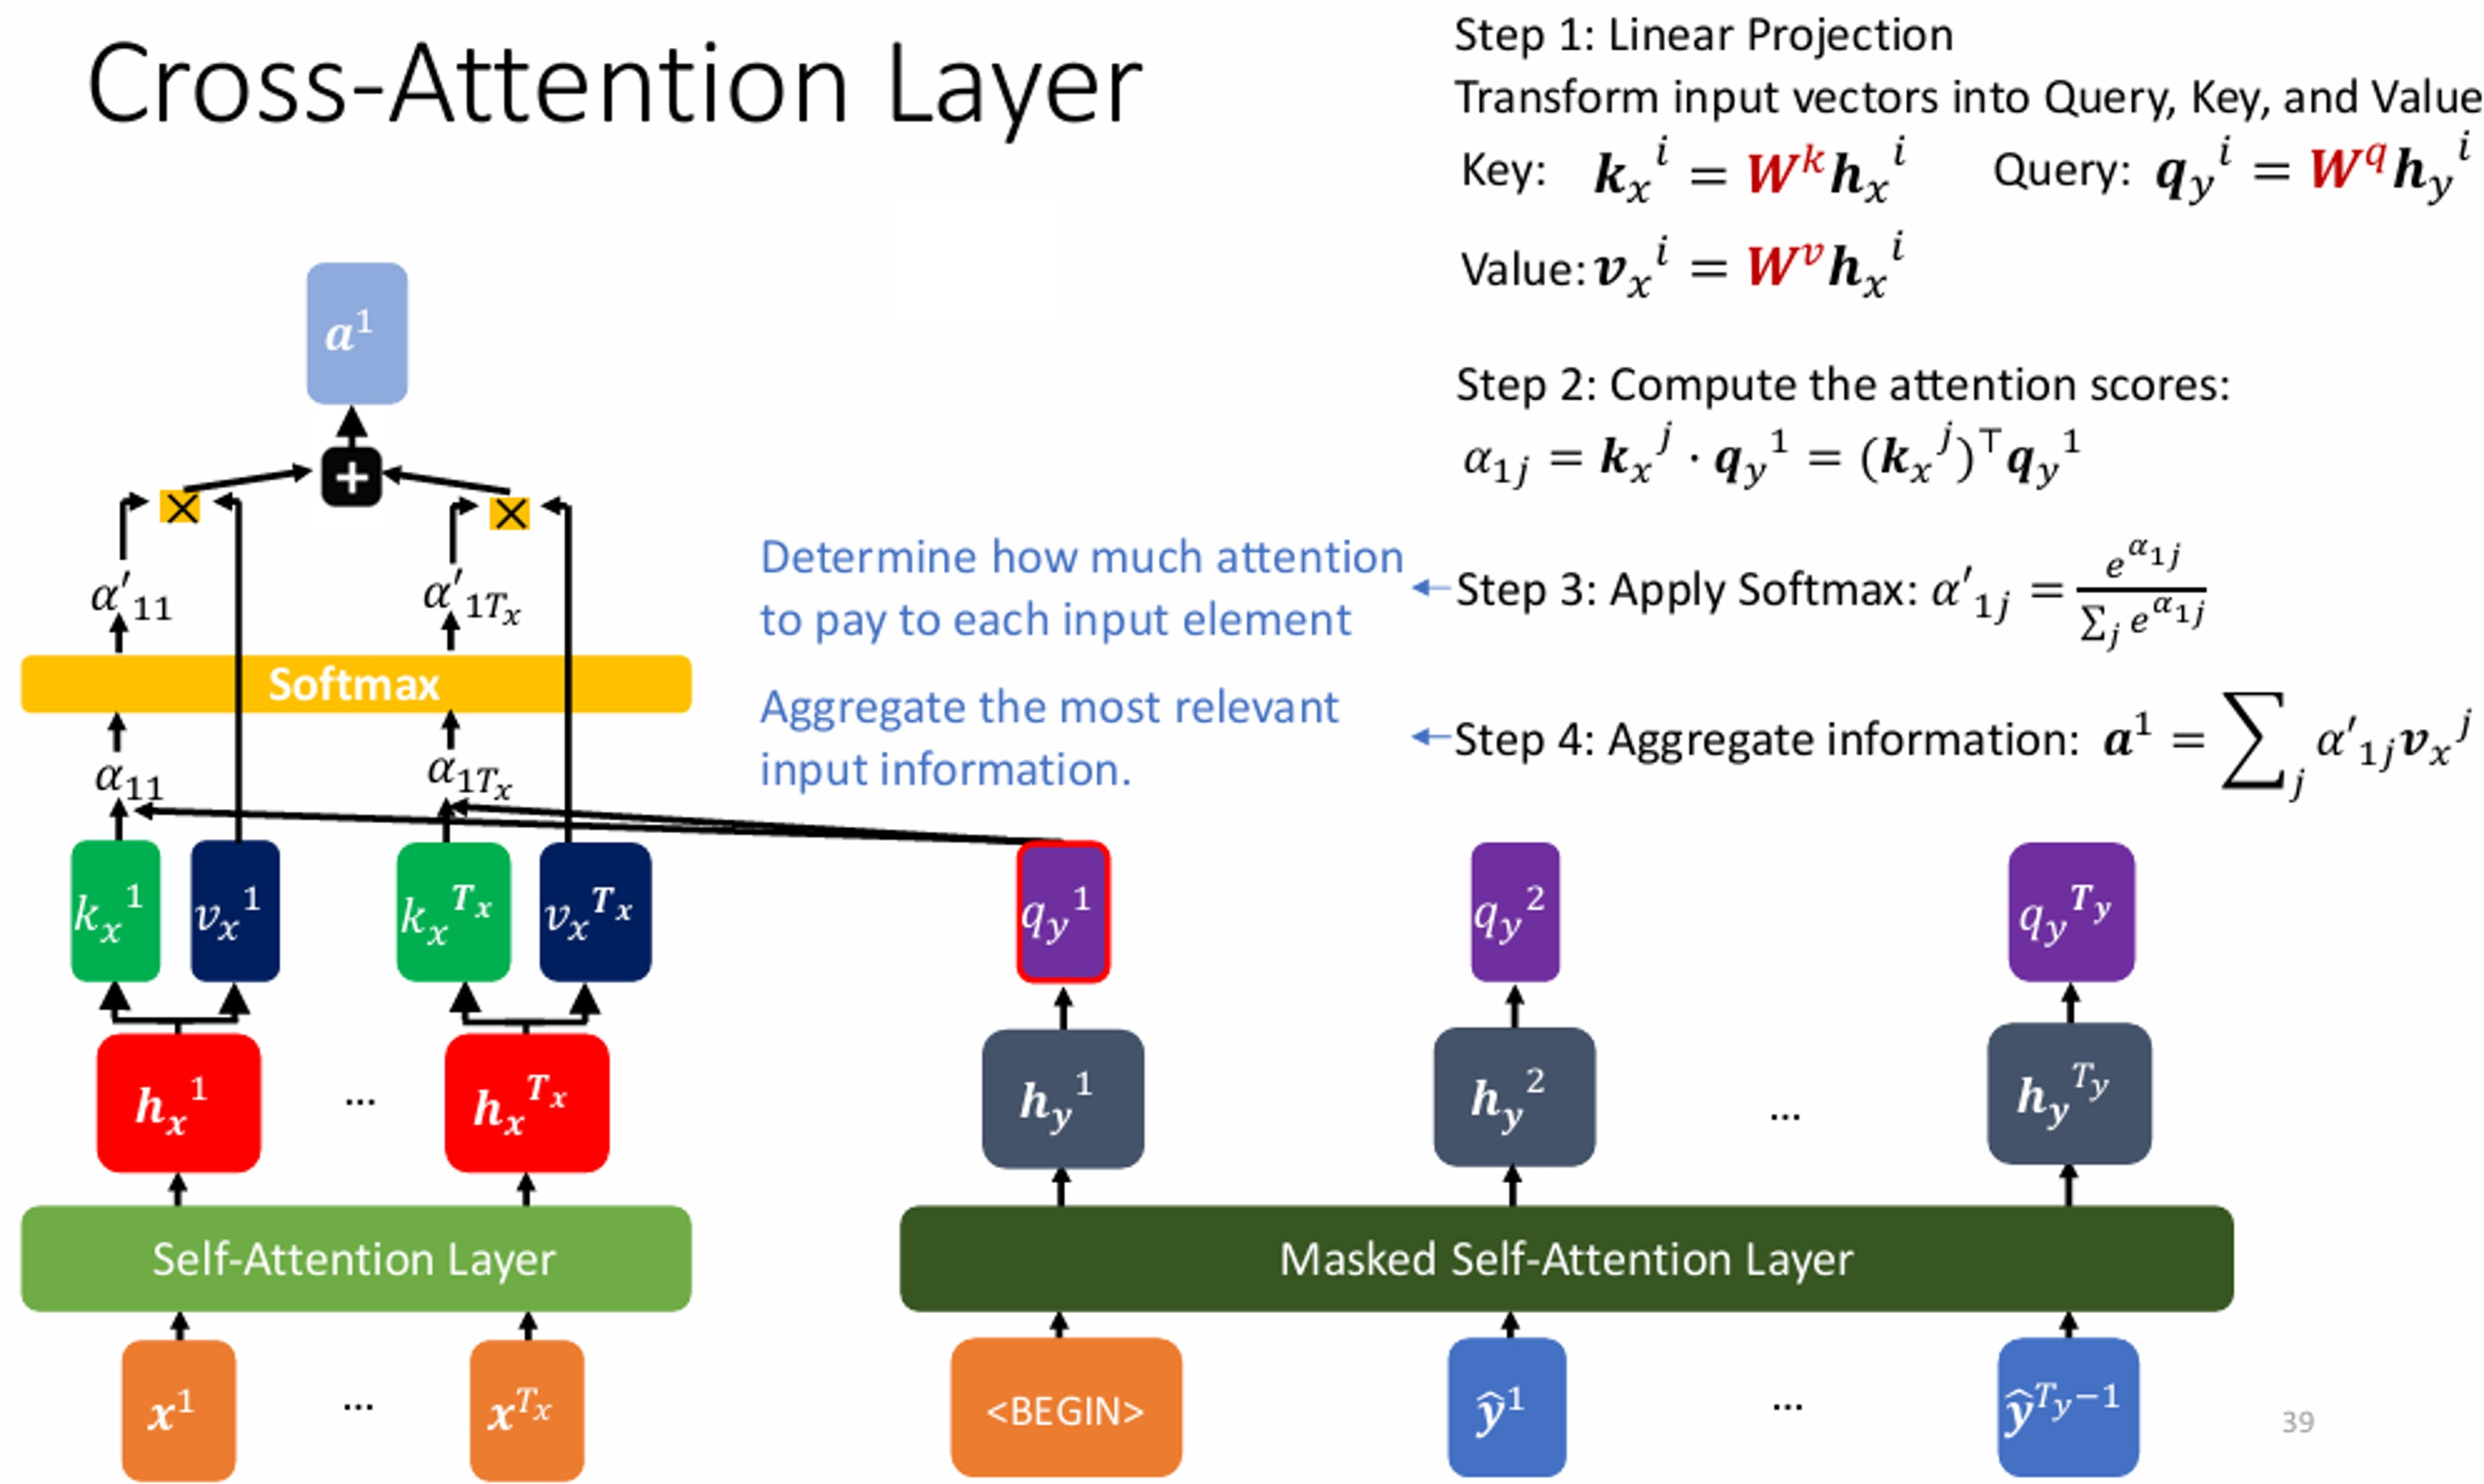
\includegraphics[width=1\linewidth]{crossAttention}}

\subsection{Transformer {\scriptsize Deep (attention-based) Neural Networks.}}
Transformer is a deep attention-based neural network architecture. Revolution sequence modeling, transduction tasks (machine translation, text generation etc.)
\begin{itemize}
\item \textbf{Key Characteristics}: Transformer relies entirely on attention mechanisms, eliminating recurrence and convolution. Composed of two main components: the \textbf{Encoder} and the \textbf{Decoder}, each consisting of multiple stacked blocks.
\item \textbf{Basic Building Blocks}:
	\begin{itemize}
	\item \textbf{Self-Attention Layer}: Capture r/s btw. all elements in \underline{input} sequence.
	\item \textbf{Feed Forward Network (FFN)}: A two-layer neural network with a ReLU activation applied independently to each position.
	\item \textbf{Masked Self-Attention Layer}: Ensures causality in autoregressive tasks by masking future tokens.
	\item \textbf{Cross-Attention Layer}: Enables the decoder to focus on relevant parts of the encoder's output.
	\item \textbf{Linear Layers}: Used for projection and transformation of inputs.
	\end{itemize}
\end{itemize}
\centerline{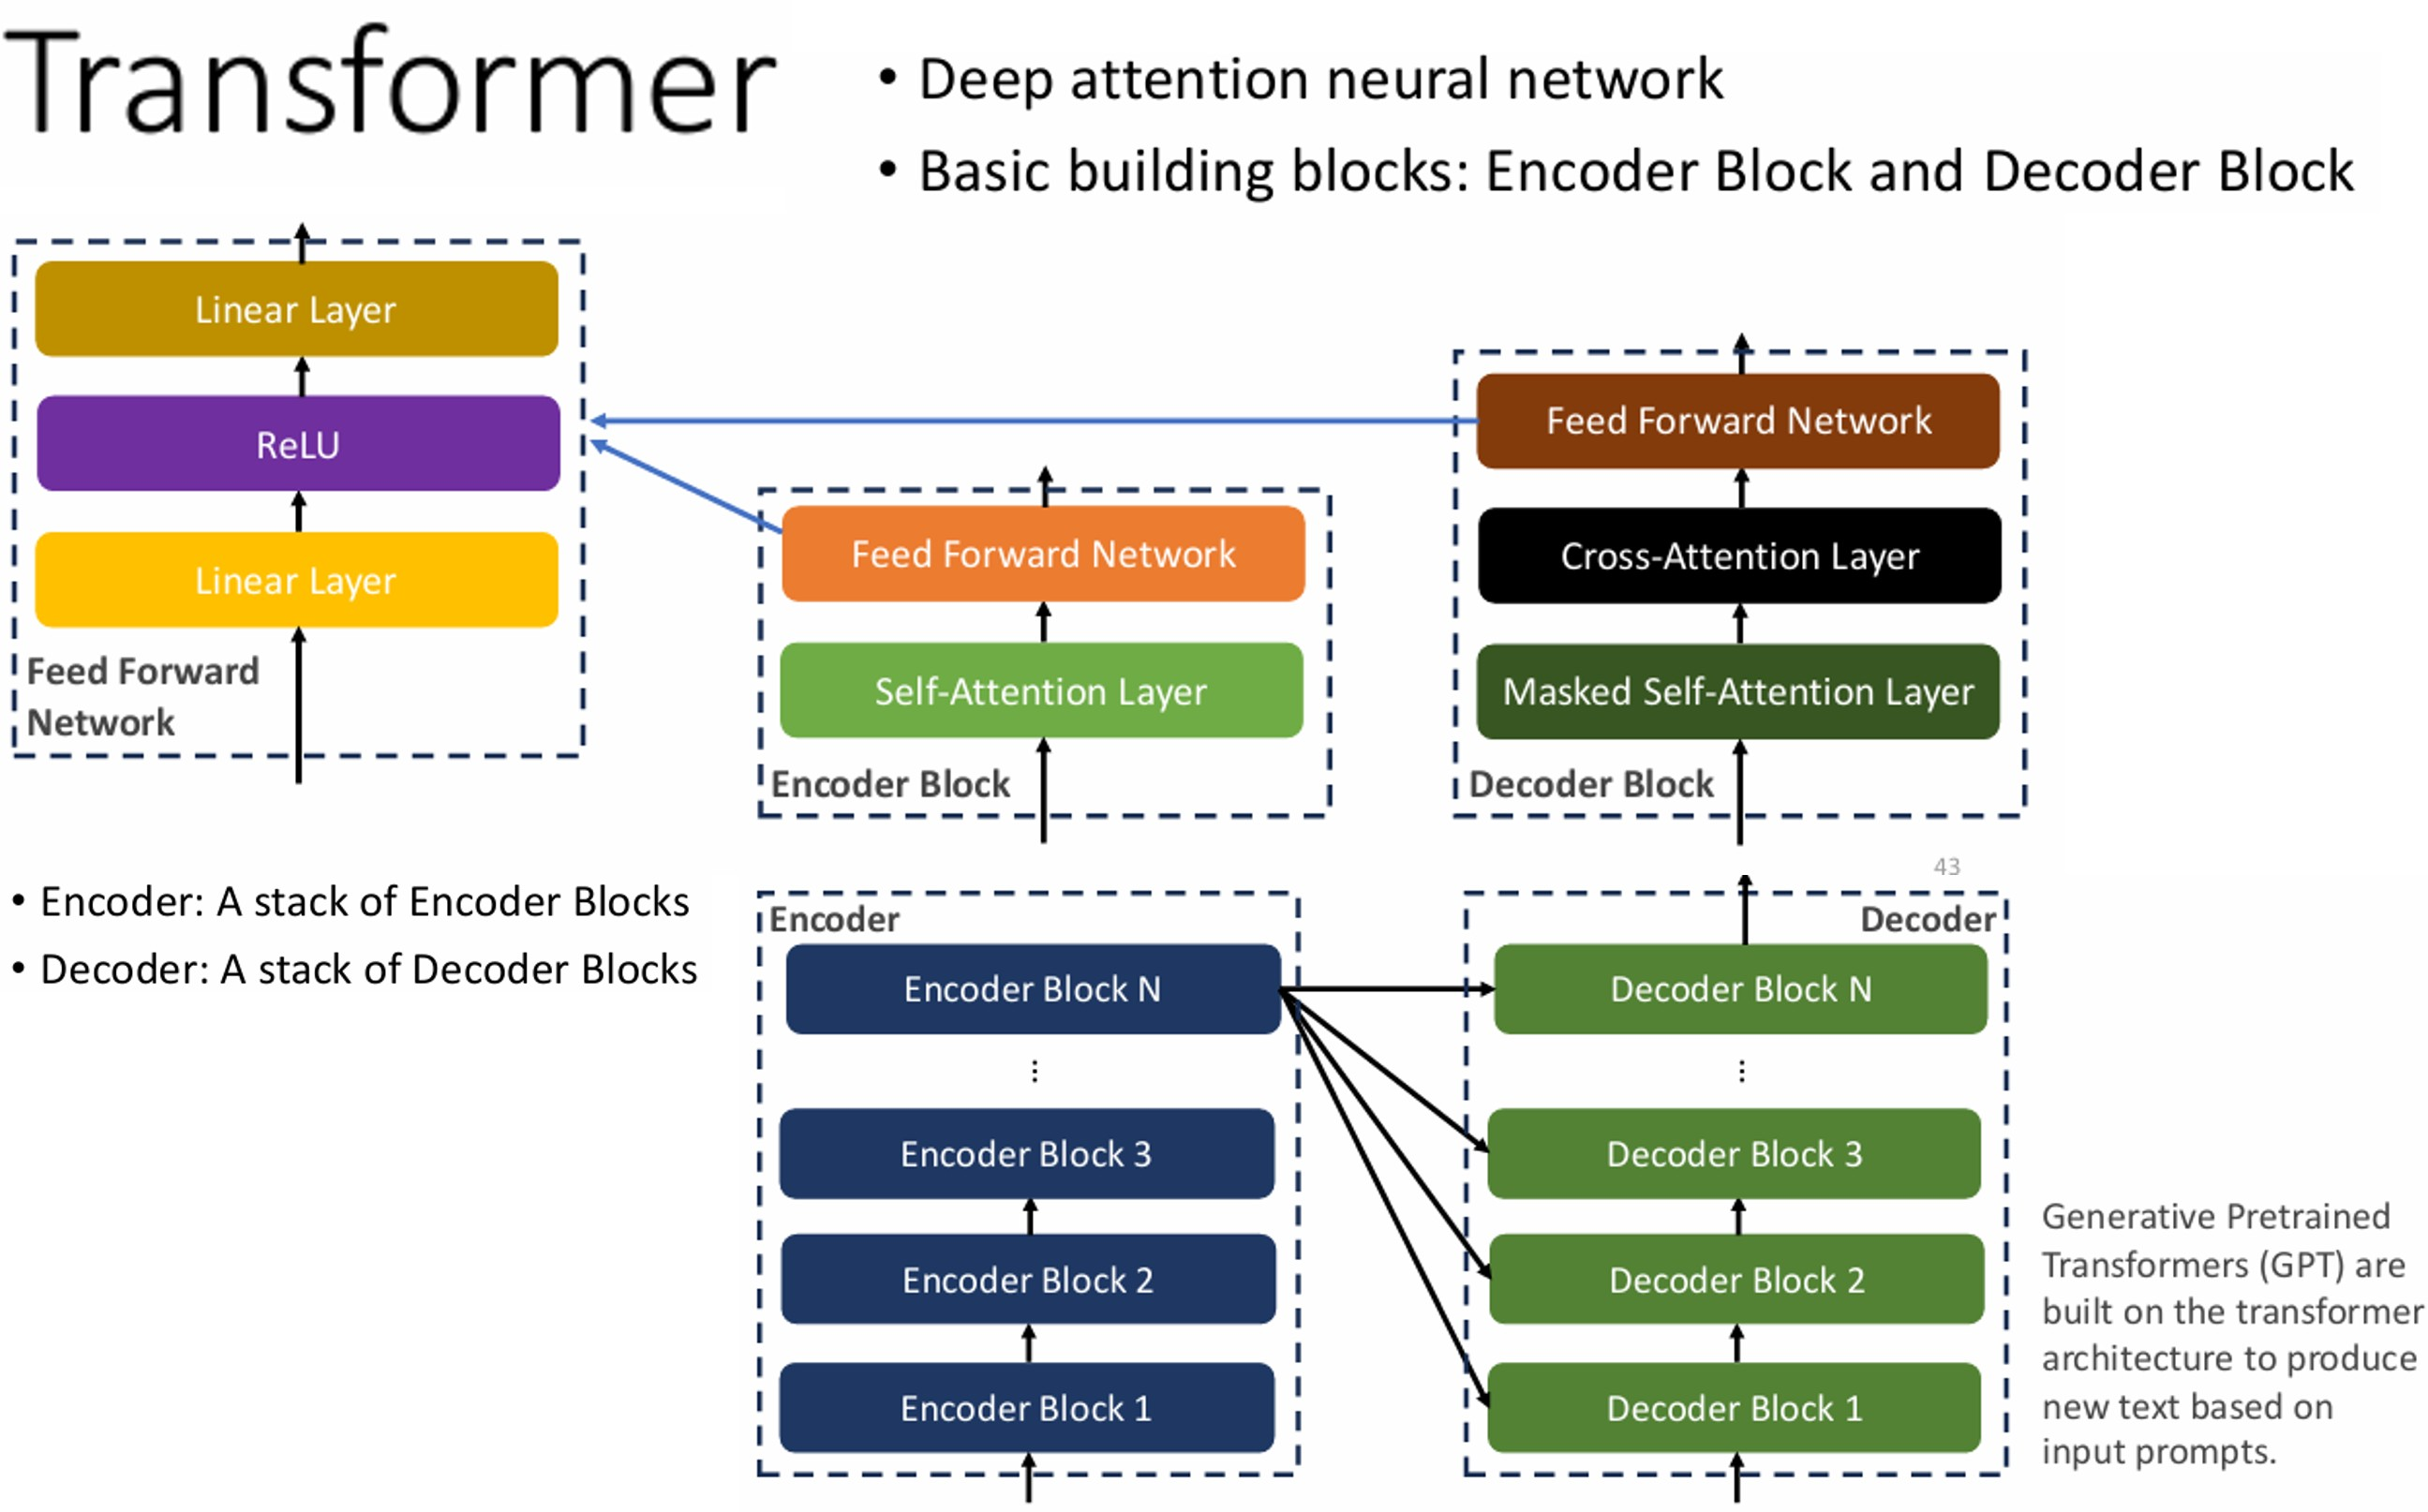
\includegraphics[width=1\linewidth]{transformer}}


\begin{itemize}
\item \textbf{Applications of Transformers}:
	\begin{itemize}
	\item \textbf{Generative Pretrained Transformers (GPT)}: Built on the Transformer architecture to generate new text based on input prompts.
	\item \textbf{Vision Transformers (ViT)}: Adapt Transformers for image classification by treating image patches as sequence elements. ($+$ Positional Encoding!) Patches are linearly embedded and combined with positional encoding to form the input sequence. A \textit{learnable summary vector} used to aggregate global information for classification tasks.
	\item Other applications include machine translation, speech recognition, and time-series forecasting.
	\end{itemize}
\end{itemize}

\subsection{15. \underline{AI Ethics}}
\begin{itemize}
\item \textbf{Ethics}: Principles guiding human behavior, distinguishing right, wrong.
\item \textbf{AI Ethics}: Principles that guide developers, manufacturers, authorities, and operators in mitigating the ethical issues arising from AI.
\item \textbf{Key Ethical Issues}: 
	\begin{itemize}
	\item \textbf{Biased Decision-Making}: AI can generate biased outputs, make unfair judgments due to biases in training data or algorithms. (E.g. Bias in AI recruiting tools, generative AI)
	\item \textbf{Manipulation of Behavior}: AI can be used to generate fake content (e.g., deepfakes) to influence human behavior and decision-making.
	\item \textbf{Automation and Employment}: AI can replace humans in certain jobs, leading to unemployment and economic inequality.
	\item \textbf{Autonomous Systems}: Autonomous systems can make decisions independently, raisie ethical questions: How should autonomous systems behave, Who is accountable for harmful actions taken.
	\item \textbf{Singularity}: Singularity in AI refers to a hypothetical future point when artificial intelligence not only reaches but exceeds human intelligence. Will the singularity ever occur? What would happen if it did occur? We still don't know. Poses existential risks and challenges, including the potential loss of human control over advanced AI systems.
	\end{itemize}
\end{itemize}



    






\end{multicols*}
\end{document}
